% Task C10
% Source volume: upper
% Physical scan pages: 316--352
% Printed book pages: 299--335
% Transcribe only source content; omit running headers, footers, and printed page numbers.
\chapter{定积分}

% BEGIN TRANSCRIPTION

这一章是一元函数积分学的基本理论。

在 §10.1 中利用可积性的三个充分必要条件对于可积函数类进行了深入讨论。§10.2 为定积分的性质，主要是积分中值定理与对积分求极限。在 §10.3 中讨论变限积分与微积分基本定理。§10.4 为定积分的计算。最后一节为学习要点和两组参考题。

定积分的应用极其广泛，将在下一章中分专题介绍。

\section{定积分概念与可积条件}

\subsection{定积分的定义}

设函数 $f$ 在区间 $[a,b]$ 上有定义。

1. 称点集 $P=\{x_0,x_1,\cdots,x_{n-1},x_n\}$ 为 $[a,b]$ 的一个\textbf{分割}，如果满足条件：
\[
  a=x_0<x_1<\cdots<x_{n-1}<x_n=b.
\]
记 $\Delta x_i=x_i-x_{i-1}$，$i=1,\cdots,n$，并称
\[
  \norm{P}=\max_{1\leqslant i\leqslant n}\{\Delta x_i\}
\]
为分割 $P$ 的\textbf{细度}。如果 $\Delta x_i=(b-a)/n$，$i=1,\cdots,n$，则称 $P$ 为等距分割。

2. 设 $P=\{x_0,x_1,\cdots,x_{n-1},x_n\}$ 为区间 $[a,b]$ 的一个分割。对每个子区间 $[x_{i-1},x_i]$，任取 $\xi_i\in[x_{i-1},x_i]$，则称 $\xi=\{\xi_i\mid i=1,2,\cdots,n\}$ 为从属于 $P$ 的一个\textbf{介点集}；并称和式
\[
  \sum_{i=1}^n f(\xi_i)\Delta x_i
  \quad\text{或}\quad
  \sum_P f(\xi_i)\Delta x_i
\]
为 $f$ 在区间 $[a,b]$ 上的一个 \textbf{Riemann（积分）和}。

3. 设 $I$ 为实数，且有
\[
  \lim_{\norm{P}\to0}\sum_{i=1}^n f(\xi_i)\Delta x_i=I,
\]
即 $\forall\varepsilon>0$，$\exists\delta>0$，对 $\norm{P}<\delta$ 的每个分割 $P$，以及对从属于 $P$ 的每个介点集 $\xi$，成立
\[
  \abs*{\sum_{i=1}^n f(\xi_i)\Delta x_i-I}<\varepsilon,
\]
则称函数 $f$ 在区间 $[a,b]$ 上 \textbf{Riemann 可积}或简称\textbf{可积}，记为
\[
  f\in R[a,b],
\]
并称 $I$ 为 $f$ 在区间 $[a,b]$ 上的 \textbf{Riemann 积分}或\textbf{定积分}，简称积分，记为
\[
  \int_a^b f(x)\,\dd x=I,
  \quad\text{或其简化记号}\quad
  \int_a^b f=I.
\]

\begin{xremark}
在上述定义中，虽然仍然是用记号 $\lim$，但是这里的极限与以前的函数极限或数列极限是不一样的。主要区别在于，在函数极限或数列极限的定义中，自变量简单地就是 $x$ 或 $n$。但这里对于每个确定的细度 $\norm{P}$，区间 $[a,b]$ 的分割 $P$ 可以有无限多个，而相对于每个 $P$，介点集 $\xi$ 的取法又有无限多个，因此就有无限多个不同的 Riemann 和。尽管如此，函数极限和数列极限的许多性质，例如，极限的唯一性、极限运算与线性运算可以交换次序等，对于这种新的极限仍然成立。
\end{xremark}

\begin{xremark}
定积分 $\int_a^b f(x)\,\dd x$ 是一个数，它的值仅仅与被积函数 $f$ 和积分区间 $[a,b]$ 有关，而与积分变量用什么符号无关，即有
\[
  \int_a^b f(x)\,\dd x=\int_a^b f(t)\,\dd t=\int_a^b f(u)\,\dd u=\cdots.
\]
因此在不需要写出积分变量时，就可以使用定积分的简化记号 $\int_a^b f$。
\end{xremark}

\subsection{可积条件}

利用积分定义中介点集的任意性就可以得到可积的一个必要条件。

\begin{xtheorem}[10.1.1]
设 $f\in R[a,b]$，则 $f$ 在 $[a,b]$ 上有界。
\end{xtheorem}
\begin{xproof}
若记 $\int_a^b f(x)\,\dd x=I$，则从可积定义知道，对于 $\varepsilon=1$，存在一个分割 $P$，使得对于从属于这个 $P$ 的任何介点集 $\xi$，均成立不等式
\begin{equation}
  \abs*{\sum_{i=1}^n f(\xi_i)\Delta x_i-I}<1.
  \tag{10.1}
  \label{eq:10.1}
\end{equation}
以下只要证明 $f$ 在每个 $I_i=[x_{i-1},x_i]$ 上有界即可。对于确定的子区间 $I_i$，固定所有 $\xi_k$（$k\ne i$），就可以从不等式 \eqref{eq:10.1} 出发对于 $f(\xi_i)$ 作出估计如下：
\[
  \frac{1}{\Delta x_i}\left(I-1-\sum_{k\ne i}f(\xi_k)\Delta x_k\right)
  <f(\xi_i)<
  \frac{1}{\Delta x_i}\left(I+1-\sum_{k\ne i}f(\xi_k)\Delta x_k\right).
\]
由于 $\xi_i\in I_i=[x_{i-1},x_i]$ 的任意性，可见 $f$ 在 $I_i$ 上有界。
\end{xproof}

为叙述可积的充分必要条件，需要引入以下概念。设函数 $f$ 在区间 $[a,b]$ 上有界，$P=\{x_0,x_1,\cdots,x_{n-1},x_n\}$ 为 $[a,b]$ 的一个分割，对 $i=1,\cdots,n$，记
\[
  M_i=\sup\{f(x)\mid x\in[x_{i-1},x_i]\},
  \qquad
  m_i=\inf\{f(x)\mid x\in[x_{i-1},x_i]\},
\]
称 $\omega_i=M_i-m_i$ 为 $f$ 在 $[x_{i-1},x_i]$ 上的\textbf{振幅}，$\sum_{i=1}^n\omega_i\Delta x_i$ 为 $f$ 的\textbf{振幅面积}。

在一般的分析教科书中对下面两个最常用的可积充分必要条件都有证明。

\begin{xtheorem}[10.1.2（可积的第一充分必要条件）]
有界函数 $f\in R[a,b]$ 的充分必要条件是
\[
  \lim_{\norm{P}\to0}\sum_{i=1}^n\omega_i\Delta x_i=0.
\]
\end{xtheorem}

\begin{xtheorem}[10.1.3（可积的第二充分必要条件）]
有界函数 $f\in R[a,b]$ 的充分必要条件是对每个 $\varepsilon>0$，存在区间 $[a,b]$ 的一个分割 $P$，使成立
\[
  \sum_P\omega_i\Delta x_i<\varepsilon.
\]
\end{xtheorem}

\begin{xremark}
条件“$\lim_{\norm{P}\to0}\sum_{i=1}^n\omega_i\Delta x_i=0$”是指“$\forall\varepsilon>0$，$\exists\delta>0$，对 $[a,b]$ 的\textbf{任意}分割 $P$，只要 $\norm{P}<\delta$，就都成立 $\sum_P\omega_i\Delta x_i<\varepsilon$”。而在可积的第二充分必要条件中，对于每一个给定的 $\varepsilon$，\textbf{只要存在一个分割} $P$ 就够了。因此，要证明给定函数的可积性，用可积的第二充分必要条件方便得多。
\end{xremark}

\begin{xremark}
在数列极限或函数极限的收敛定义中，似乎没有与上述第二充分必要条件对应的结果，但是对于单调数列（以及单调函数）却有类似的结果。例如，单调增加数列 $\{x_n\}$ 收敛于数 $a$ 的充分必要条件是：对每个 $\varepsilon>0$，存在数列的某一项 $x_N$，使成立 $a-\varepsilon<x_N\leqslant a$。这个结果已用于例题 3.1.1 中。这个类比并非偶然。可积的第二充分必要条件就是来源于 Riemann 和对于分割的某种“单调性”。对此有兴趣的读者可以参考 [14] 第三卷附录中的 Moore-Smith 收敛。
\end{xremark}

利用上面的充分必要条件，就可以证明关于 Riemann 可积函数类的三个结论：
\begin{enumerate}
  \item 设 $f\in C[a,b]$，则 $f\in R[a,b]$；
  \item 设 $f$ 在 $[a,b]$ 上有界且只有有限个间断点，则 $f\in R[a,b]$；
  \item 设 $f$ 在 $[a,b]$ 上单调，则 $f\in R[a,b]$。
\end{enumerate}

另一方面，设 $D(x)$ 为 Dirichlet 函数（见 4.1.5 小节题 11），则对任意区间 $[a,b]$ 以及 $[a,b]$ 的任意分割 $P$，当 $\xi_i$ 均取有理数时，有 $\sum_P f(\xi_i)\Delta x_i=b-a$，而当 $\xi_i$ 均取无理数时，则有 $\sum_P f(\xi_i)\Delta x_i=0$。因此振幅面积总是等于 $b-a$。由此可见，Dirichlet 函数在任何有界区间 $[a,b]$ 上都不可积。

下面是另一个可积的充分必要条件，它在讨论较为复杂的函数的可积性时，往往比可积的第二充分必要条件更为方便。

\begin{xtheorem}[10.1.4（可积的第三充分必要条件）]
有界函数 $f\in R[a,b]$ 的充分必要条件是 $\forall\varepsilon,\eta>0$，存在 $[a,b]$ 的分割 $P$，使振幅不小于 $\eta$ 的子区间的长度之和小于 $\varepsilon$。
\end{xtheorem}
\begin{xproof}
设在 $[a,b]$ 上有 $m\leqslant f(x)\leqslant M$。

先证充分性。对于 $\varepsilon>0$，取
\[
  \varepsilon'=\frac{\varepsilon}{2(M-m)},
  \qquad
  \eta=\frac{\varepsilon}{2(b-a)}.
\]
根据条件，存在 $[a,b]$ 的分割 $P$，使振幅不小于 $\eta$ 的子区间的长度之和小于 $\varepsilon'$（见图 10.1）。对 $P$，用 $\sum'$ 和 $\sum''$ 分别表示在积分和式中对振幅不小于 $\eta$ 的子区间和对振幅小于 $\eta$ 的子区间求和。我们有
\[
  \sum'\omega_i\Delta x_i\leqslant(M-m)\sum'\Delta x_i<(M-m)\varepsilon',
\]
\[
  \sum''\omega_i\Delta x_i<\eta\sum''\Delta x_i<\eta(b-a).
\]
合并得到
\[
  \sum\omega_i\Delta x_i<(M-m)\varepsilon'+\eta(b-a)<\varepsilon.
\]
由可积的第二充分必要条件可见 $f$ 在 $[a,b]$ 上 Riemann 可积。

再证必要性。设 $f$ 在 $[a,b]$ 上 Riemann 可积，则由可积的第二充分必要条件，对给定的 $\varepsilon,\eta>0$，存在 $[a,b]$ 的分割 $P$，使 $\sum_P\omega_i\Delta x_i<\varepsilon\eta$。用 $\sum'$ 表示对振幅不小于 $\eta$ 的子区间求和，则
\[
  \eta\sum'\Delta x_i\leqslant\sum'\omega_i\Delta x_i\leqslant\sum_P\omega_i\Delta x_i<\varepsilon\eta.
\]
因此 $\sum'\Delta x_i<\varepsilon$，即振幅不小于 $\eta$ 的子区间的长度之和小于 $\varepsilon$。
\end{xproof}

\begin{center}
  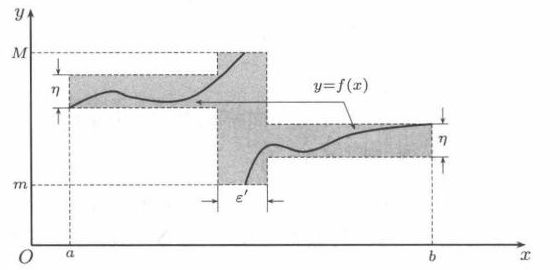
\includegraphics[width=.62\linewidth]{figures/upper/ch10/fig-10-1.png}

  图 10.1
\end{center}

对于有无限多个间断点的函数，用可积的第三充分必要条件来讨论其可积性比较容易。

\begin{xexample}[10.1.1]
证明函数
\[
  f(x)=
  \begin{cases}
    \dfrac1x-\left[\dfrac1x\right],&x\in(0,1],\\
    0,&x=0
  \end{cases}
\]
在 $[0,1]$ 上可积。
\end{xexample}
\begin{xsolution}
\textbf{分析}\quad 虽然 $f$ 在 $[0,1]$ 内有无限个间断点，然而由于这些间断点可以看成为收敛于 0 的数列，因此可用总长度任意小的有限个区间把所有间断点覆盖住，这就是下列证明的要点。

对给定的 $\varepsilon,\eta>0$ 取 $n$ 充分大，使得
\[
  \delta=\frac1{n+\frac12}<\frac\varepsilon2.
\]
将区间 $[0,1]$ 分成 $[0,\delta)$ 和 $[\delta,1]$。$f$ 在 $[\delta,1]$ 内的所有间断点是 $\{1/i\mid i=2,\cdots,n\}$。用包含于 $(\delta,1]$ 中的 $n-1$ 个互不相交的开区间覆盖这些间断点，并要求这些开区间的总长度小于 $\varepsilon/2$（见图 10.2）。从 $[0,1]$ 中挖掉这些子区间与 $[0,\delta)$，剩余的部分是 $n$ 个闭子区间。因为 $f$ 在这些闭子区间上一致连续，因此我们能够将这些子区间细分为更小的子区间，使 $f$ 在每个子区间上的振幅都小于 $\eta$。上面所有子区间的端点构成 $[0,1]$ 的一个分割。其中振幅不小于 $\eta$ 的子区间的长度之和小于 $\varepsilon$，由可积的第三充分必要条件可知 $f\in R[a,b]$。
\end{xsolution}

\begin{center}
  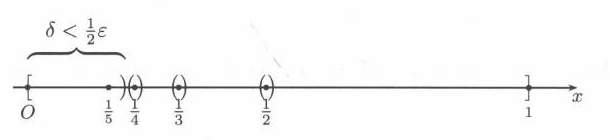
\includegraphics[width=.68\linewidth]{figures/upper/ch10/fig-10-2.png}

  图 10.2
\end{center}

这样我们就看到 Riemann 可积函数可以有无限多个不连续点。不仅如此，这些不连续点的分布还可能比例题 10.1.1 中的情况复杂得多。例如，例题 5.1.4 中的 Riemann 函数以所有的有理数点为间断点，但它仍然是可积函数（留作 10.1.3 小节的练习题 10）。

这里要注意，虽然有理数在数轴上处处稠密，但仍然可以用总长度任意小的开区间族来覆盖。不过这时开区间的个数不是有限个，而是可列个。关键是用有理数的可列性，先将它们记为一个数列 $\{r_n\}$。对于给定的 $\varepsilon>0$，用长度 $\frac12\varepsilon$ 的开区间覆盖点 $r_1$，用长度 $\frac14\varepsilon$ 的开区间覆盖 $r_2$，$\cdots$，用长度 $\frac1{2^n}\varepsilon$ 的开区间覆盖 $r_n$，如此进行下去，就可以覆盖所有有理数，而所用的开区间的总长度不超过 $\varepsilon$。

从可积的第三充分必要条件不难得到下面对于可积函数的很一般的刻画。

\begin{xtheorem}[10.1.5]
设函数 $f$ 在区间 $[a,b]$ 上有界，如果 $f$ 的所有不连续点可以用总长度任意小的至多可列个开区间覆盖，则 $f\in R[a,b]$。
\end{xtheorem}
\begin{xproof}
对于给定的 $\varepsilon,\eta>0$，先用总长度小于 $\varepsilon$ 的有限个或可列个开区间覆盖 $f$ 的所有不连续点；然后对于每个连续点，设为 $x_0$，用一个邻域 $O(x_0)$ 覆盖，且要求 $f$ 在这个邻域上的振幅小于 $\eta$。由于 $f$ 在点 $x_0$ 的连续性，这是能够满足的。

对于每个连续点都取这样的邻域，于是所有这些邻域和覆盖不连续点的开区间一起就构成为区间 $[a,b]$ 的一个开覆盖，记为 $\{O_\alpha\}$。

利用加强形式的覆盖定理（即例题 3.5.3），存在 Lebesgue 数 $\delta$，使得在区间 $[a,b]$ 中的相距不超过 $\delta$ 的任何两点可以用开覆盖 $\{O_\alpha\}$ 中的某一个开区间同时覆盖。

对于区间 $[a,b]$ 取细度不超过 $\delta$ 的等距分割 $P$。这时每个子区间被开覆盖中的一个开区间所覆盖。如果子区间是由原来覆盖不连续点的开区间所覆盖，则这类子区间的总长度必小于 $\varepsilon$。而覆盖所有其他子区间的开区间都是原先用于覆盖连续点的邻域，因此 $f$ 在每一个这类子区间上的振幅小于 $\eta$。

根据可积的第三充分必要条件，可知 $f$ 在 $[a,b]$ 上可积。
\end{xproof}

\begin{xremark}
在实变函数论中，如果一个点集可以用总长度任意小的至多可列个开区间覆盖，就称这个点集为\textbf{零测度集}。如果某种性质在一个零测度集之外成立，就说这个性质\textbf{几乎处处成立}。应用这些术语，我们就可以叙述实变函数论中的 Lebesgue 定理，它给出了 Riemann 可积函数的完整刻画，非常有用。
\end{xremark}

\begin{xtheorem}[10.1.6（Lebesgue 定理）]
若函数 $f$ 在 $[a,b]$ 上有界，则 $f\in R[a,b]$ 的充分必要条件是 $f$ 在 $[a,b]$ 上几乎处处连续。
\end{xtheorem}
\begin{xproof}
这个定理的充分性部分就是上面的命题 10.1.5。其必要性证明简述如下（对细节有兴趣的读者可以参考 [8]）。

设 $f\in R[a,b]$，则从可积的第三充分必要条件可知，对于 $\varepsilon,\eta>0$，存在分割 $P$，使得其中振幅不小于 $\eta$ 的子区间的长度之和小于 $\varepsilon$。利用函数在一点的振幅概念（见 5.1.1 小节的第 5 点），可见 $f$ 的振幅超过 $\eta$ 的不连续点或者落在振幅超过 $\eta$ 的子区间内（而所有这类子区间的总长度小于 $\varepsilon$），或者是分割 $P$ 的某些分点。再增加几个长度充分小的开区间来覆盖这些分点，就可以用总长度小于 $\varepsilon$ 的有限个开区间将所有振幅超过 $\eta$ 的不连续点全部覆盖住。

现在取 $\eta_n=1/2^n$，$\varepsilon_n=\varepsilon/2^n$，并对每个 $n$ 重复以上过程，就可用总长度不超过 $\varepsilon$ 的至多可列个开区间覆盖 $f$ 的所有不连续点。由于这对每个 $\varepsilon>0$ 都能做到，因此 $f$ 在 $[a,b]$ 上几乎处处连续。
\end{xproof}

\subsection{练习题}

对下面的前 10 个题来说，每题至少可以举出两个解法。其中的一个解法是从定积分定义出发，而另一个解法则是以 Lebesgue 定理（命题 10.1.6）为根据的。这两种解法的思路很不一样。初学者通过这样的训练既可以熟悉定积分的基本出发点，又可以学会如何应用 Lebesgue 定理和有关的概念去处理一般的 Riemann 可积函数。对于今后遇到的有关可积函数的问题都可以如此考虑。

\begin{xexercise}[1]
设
\[
  f(x)=
  \begin{cases}
    x(1-x),&x\text{ 是有理数},\\
    0,&x\text{ 是无理数}.
  \end{cases}
\]
问 $f$ 在 $[0,1]$ 上是否可积？
\end{xexercise}
\begin{xsolution}
不可积。事实上，在任意 $x_0\in(0,1)$ 处，由有理数与无理数的稠密性，均可取有理数列 $r_n\to x_0$ 与无理数列 $s_n\to x_0$。于是
\[
  f(r_n)\to x_0(1-x_0)>0,
  \qquad
  f(s_n)=0,
\]
故 $f$ 在每个 $x_0\in(0,1)$ 处都不连续。另一方面，在 $0,1$ 两点有
\[
  \abs{f(x)}\leqslant x(1-x)\to0,
\]
所以 $f$ 只在端点连续。

因此 $f$ 的不连续点集为 $(0,1)$，不是零测度集。由 Lebesgue 判别定理（命题 10.1.6），$f\notin R[0,1]$。
\end{xsolution}


\begin{xexercise}[2]
设 $f,g\in R[a,b]$，且 $f$ 的值域在 $[a,b]$ 中，问 $g\circ f$ 在 $[a,b]$ 上是否可积？又若 $f,g$ 在 $[a,b]$ 上都不可积，问 $g\circ f$ 在 $[a,b]$ 上是否一定不可积？
\end{xexercise}
\begin{xsolution}
第一个问题的答案是否定的。取 $[a,b]=[0,1]$，令 $f$ 为 Riemann 函数（Thomae 函数）
\[
  f(x)=
  \begin{cases}
    1/q,&x=p/q\in[0,1]\text{，且 }(p,q)=1,\\
    0,&x\text{ 为无理数},
  \end{cases}
\]
则 $f\in R[0,1]$，且 $f([0,1])\subseteq[0,1]$。再令
\[
  g(y)=
  \begin{cases}
    1,&y=0,\\
    0,&y\ne0.
  \end{cases}
\]
函数 $g$ 只在 $0$ 处与零函数不同，故 $g\in R[0,1]$。但
\[
  (g\circ f)(x)=
  \begin{cases}
    0,&x\text{ 为有理数},\\
    1,&x\text{ 为无理数},
  \end{cases}
\]
是 Dirichlet 型函数，在每一点都不连续，因而不可积。

第二个问题的答案也是否定的。仍在 $[0,1]$ 上令
\[
  f(x)=g(x)=
  \begin{cases}
    1,&x\text{ 为有理数},\\
    0,&x\text{ 为无理数}.
  \end{cases}
\]
则 $f,g$ 都不可积，而 $f(x)$ 只取 $0,1$ 两值，且 $g(0)=g(1)=1$，所以
\[
  (g\circ f)(x)\equiv1,
\]
反而是可积函数。
\end{xsolution}


\begin{xexercise}[3]
讨论区间 $[a,b]$ 上 $f$，$\abs{f}$，$f^2$ 的可积性之间的关系。
\end{xexercise}
\begin{xsolution}
有如下关系：
\[
  f\in R[a,b]\Longrightarrow \abs{f}\in R[a,b]
  \Longleftrightarrow f^2\in R[a,b].
\]
第一步是因为绝对值函数连续，连续函数与 Riemann 可积函数的复合仍可积。若 $\abs f\in R[a,b]$，则
\[
  f^2=(\abs f)^2\in R[a,b].
\]
反之，若 $f^2\in R[a,b]$，则 $f^2\geqslant0$，而平方根函数在 $[0,+\infty)$ 上连续，所以
\[
  \abs f=\sqrt{f^2}\in R[a,b].
\]

反向推出 $f$ 一般不成立。例如在任意非退化区间上令
\[
  f(x)=
  \begin{cases}
    1,&x\text{ 为有理数},\\
    -1,&x\text{ 为无理数},
  \end{cases}
\]
则 $f$ 处处不连续，从而不可积，但
\[
  \abs f\equiv1,\qquad f^2\equiv1
\]
均可积。
\end{xsolution}


\begin{xexercise}[4]
设 $f\in R[a,b]$，$g$ 与 $f$ 在 $[a,b]$ 上仅在有限个点上取不同值，证明：$g\in R[a,b]$，并且
\[
  \int_a^b f=\int_a^b g.
\]
又问：如果 $f$ 和 $g$ 在 $[a,b]$ 上几乎处处相等，例如只在所有有理数点上的函数值不同，则是否有相同结论？\footnote{因此对于在 $[a,b]$ 上的有界函数，如果它在有限个点上没有定义，我们可以采取补充定义的方法进行讨论。这时的可积性和可积时的积分值与补充定义的具体做法无关。}
\end{xexercise}
\begin{xsolution}
先设 $f,g$ 只在有限个点 $x_1,\ldots,x_N$ 上不同。令 $h=g-f$。则 $h$ 只在有限点可能非零，因此 $h\in R[a,b]$ 且
\[
  \int_a^b h(x)\,\dd x=0.
\]
于是
\[
  g=f+h\in R[a,b],
  \qquad
  \int_a^b g=\int_a^b f.
\]

若只把“有限个点”放宽为“几乎处处相等”，则一般不能推出相同结论。反例取
\[
  f(x)\equiv0,
  \qquad
  g(x)=
  \begin{cases}
    1,&x\in\QQ,\\
    0,&x\notin\QQ,
  \end{cases}
  \qquad x\in[a,b].
\]
有理数集为零测度集，所以 $f=g$ 几乎处处；但 $f\in R[a,b]$，而 $g$ 是 Dirichlet 型函数，在每一点都不连续，故 $g\notin R[a,b]$。

如果另加条件 $g\in R[a,b]$，则积分值仍然相同。事实上 $h=g-f\in R[a,b]$ 且 $h=0$ 几乎处处，因此 $\int_a^b h=0$，从而 $\int_a^b f=\int_a^b g$。
\end{xsolution}


\begin{xexercise}[5]
设 $f\in R[a,b]$，且对每个 $(\alpha,\beta)\subseteq[a,b]$，$\exists x_1,x_2\in(\alpha,\beta)$，使 $f(x_1)f(x_2)\leqslant0$，问定积分 $\int_a^b f$ 的值是多少？为什么？
\end{xexercise}
\begin{xsolution}
所求积分为 $0$。

由于 $f\in R[a,b]$，由 Lebesgue 判别定理，$f$ 的连续点在 $[a,b]$ 中稠密。设 $x_0$ 是一个连续点。若 $f(x_0)>0$，由连续性存在包含 $x_0$ 的小区间 $(\alpha,\beta)$，使其中恒有 $f(x)>0$。于是任意 $x_1,x_2\in(\alpha,\beta)$ 都满足
\[
  f(x_1)f(x_2)>0,
\]
与题设矛盾。同理不可能有 $f(x_0)<0$。故 $f$ 在每个连续点上都等于 $0$。

因此 $f=0$ 几乎处处，而 $f$ Riemann 可积，故
\[
  \boxed{\int_a^b f(x)\,\dd x=0}.
\]
\end{xsolution}


\begin{xexercise}[6]
设 $g\in R[a,b]$，$M=\sup_{x\in[a,b]}\{g(x)\}$，$m=\inf_{x\in[a,b]}\{g(x)\}$，如果 $m<M$，$f\in C[m,M]$，证明：$f\circ g\in R[a,b]$。
\end{xexercise}
\begin{xsolution}
因为 $g\in R[a,b]$，故 $g$ 有界，且其不连续点集为零测度集。题设给出
\[
  m\leqslant g(x)\leqslant M.
\]
函数 $f\in C[m,M]$ 在紧区间上连续，从而一致连续。若 $x_0$ 是 $g$ 的连续点，则
\[
  g(x)\to g(x_0)\quad(x\to x_0)
\]
立即推出
\[
  f(g(x))\to f(g(x_0)),
\]
所以 $f\circ g$ 在 $x_0$ 连续。因此
\[
  D(f\circ g)\subseteq D(g),
\]
其中 $D(\cdot)$ 表示不连续点集。右边为零测度集，而且 $f\circ g$ 有界。由 Lebesgue 判别定理，
\[
  f\circ g\in R[a,b].
\]
\end{xsolution}


\begin{xexercise}[7]
设 $f\in R[a,b]$，且 $1/f$ 在 $[a,b]$ 上有界，证明：$1/f\in R[a,b]$。
\end{xexercise}
\begin{xsolution}
由 $1/f$ 在 $[a,b]$ 上有界，存在常数 $C>0$，使
\[
  \abs*{\frac1{f(x)}}\leqslant C,
\]
故
\[
  \abs{f(x)}\geqslant c:=\frac1C>0.
\]
函数 $\varphi(y)=1/y$ 在集合
\[
  (-\infty,-c]\cup[c,+\infty)
\]
上连续，而且在 $f([a,b])$ 上一致连续。于是 $f$ 的每个连续点也是 $1/f$ 的连续点。因此
\[
  D(1/f)\subseteq D(f).
\]
因 $f\in R[a,b]$，$D(f)$ 为零测度集；同时 $1/f$ 已知有界。由 Lebesgue 判别定理即得
\[
  \frac1f\in R[a,b].
\]
\end{xsolution}


\begin{xexercise}[8]
设 $f$ 在 $[a,b]$ 上有界，且其所有间断点构成一个收敛数列，证明：$f\in R[a,b]$。
\end{xexercise}
\begin{xsolution}
设 $f$ 的所有间断点组成收敛数列 $\{x_n\}$；若极限点本身未列入数列，把它补入也只增加一个点。于是 $f$ 的不连续点集至多可列，因而为零测度集。题设又给出 $f$ 在 $[a,b]$ 上有界，所以由 Lebesgue 判别定理
\[
  f\in R[a,b].
\]
\end{xsolution}


\begin{xexercise}[9]
设 $f$ 在区间 $[a,b]$ 的每一点的极限都存在且为零，证明：$f\in R[a,b]$ 且 $\int_a^b f=0$。
\end{xexercise}
\begin{xsolution}
对每个 $x_0\in[a,b]$，题设给出
\[
  \lim_{x\to x_0}f(x)=0.
\]
先证 $f$ 有界。对每个 $x_0$，存在邻域 $U_{x_0}$，使在 $U_{x_0}\cap[a,b]$ 内（除去 $x_0$ 本身）有 $\abs{f(x)}<1$。加上点值 $f(x_0)$ 后，$f$ 在每个这样的邻域上有界。利用 $[a,b]$ 的紧致性取有限子覆盖，即知 $f$ 在整个 $[a,b]$ 上有界。

再看非零点集。对任意 $n\in\NN_+$，令
\[
  E_n=\{x\in[a,b]\mid \abs{f(x)}\geqslant1/n\}.
\]
$E_n$ 不可能有聚点：若 $x_k\in E_n$ 且 $x_k\to x_0$、$x_k\ne x_0$，则由题设应有 $f(x_k)\to0$，矛盾。紧区间中的无限集合必有聚点，所以每个 $E_n$ 都是有限集。于是
\[
  \{x\mid f(x)\ne0\}=\bigcup_{n=1}^\infty E_n
\]
至多可列。

若 $f(x_0)=0$，由极限也为 $0$ 可知 $f$ 在 $x_0$ 连续；若 $f(x_0)\ne0$，则该点是不连续点。因此 $f$ 的不连续点集至多可列。由 Lebesgue 判别定理，$f\in R[a,b]$。又 $f=0$ 几乎处处，故
\[
  \boxed{\int_a^b f(x)\,\dd x=0}.
\]
\end{xsolution}


\begin{xexercise}[10]
证明：Riemann 函数（见例题 5.1.4）在每个有界区间 $[a,b]$ 上可积。
\end{xexercise}
\begin{xsolution}
Riemann 函数在任意有界区间上有界；由本章正文已知，它恰在有理点处不连续，而在无理点处连续。有理数集至多可列，因而为零测度集。故由 Lebesgue 判别定理，Riemann 函数在每个有界区间 $[a,b]$ 上 Riemann 可积。

并且它在所有无理数点取值为 $0$，故也有
\[
  \int_a^b f(x)\,\dd x=0.
\]
\end{xsolution}


\begin{xexercise}[11]
对连续函数，能否如下定义定积分：如果 $f\in C[a,b]$ 且存在实数 $I$，使
\[
  \lim_{n\to\infty}\frac{b-a}{n}\sum_{i=1}^n f\left(a+\frac{i}{n}(b-a)\right)=I,
\]
则 $f\in R[a,b]$ 且 $\int_a^b f=I$。
\end{xexercise}
\begin{xsolution}
可以。事实上，对连续函数，这种等距分割右端点和确实足以确定定积分。

设
\[
  S_n=\frac{b-a}{n}\sum_{i=1}^n
  f\left(a+\frac{i}{n}(b-a)\right).
\]
由于 $f\in C[a,b]$，$f$ 在 $[a,b]$ 上一致连续。令等距分割的步长为
\[
  \Delta_n=\frac{b-a}{n}.
\]
任取从属于该分割的介点 $\xi_i$，则
\[
  \abs*{S_n-\sum_{i=1}^n f(\xi_i)\Delta_n}
  \leqslant
  \sum_{i=1}^n
  \abs*{f\left(a+i\Delta_n\right)-f(\xi_i)}\Delta_n.
\]
当 $n$ 充分大时，每个 $\abs{a+i\Delta_n-\xi_i}\leqslant\Delta_n$ 都很小；由一致连续性，右端可任意小。另一方面，连续函数 Riemann 可积，任意介点 Riemann 和都趋于 $\int_a^b f$。因此
\[
  \lim_{n\to\infty}S_n=\int_a^b f(x)\,\dd x.
\]
若题设又给出 $S_n\to I$，由极限唯一性即得
\[
  I=\int_a^b f(x)\,\dd x.
\]
\end{xsolution}


\begin{xexercise}[12]
设 $f,g\in R[a,b]$，$P=\{x_0,x_1,\cdots,x_n\}$ 是区间 $[a,b]$ 的分割，证明：$\forall\varepsilon>0$，$\exists\delta>0$，使对于满足 $\norm{P}<\delta$ 的任意分割 $P$，成立
\[
  \abs*{\sum_{k=1}^n f(x_k)\sin(g(x_k)\Delta x_k)-\int_a^b f(x)g(x)\,\dd x}<\varepsilon.
\]
\end{xexercise}
\begin{xsolution}
由于 $f,g\in R[a,b]$，二者都有界，且乘积 $fg\in R[a,b]$。取常数 $A,B>0$，使
\[
  \abs{f(x)}\leqslant A,
  \qquad
  \abs{g(x)}\leqslant B.
\]
记
\[
  S_P=\sum_{k=1}^n f(x_k)\sin(g(x_k)\Delta x_k),
  \qquad
  T_P=\sum_{k=1}^n f(x_k)g(x_k)\Delta x_k.
\]
利用
\[
  \abs{\sin u-u}\leqslant\frac{\abs u^3}{6},
\]
有
\begin{align*}
  \abs{S_P-T_P}
  &\leqslant\frac{A}{6}\sum_{k=1}^n
    \abs{g(x_k)}^3(\Delta x_k)^3\\
  &\leqslant\frac{AB^3}{6}\norm P^2\sum_{k=1}^n\Delta x_k\\
  &=\frac{AB^3(b-a)}6\norm P^2.
\end{align*}
故当 $\norm P\to0$ 时，$S_P-T_P\to0$。而 $T_P$ 是 $fg$ 的右端点 Riemann 和，所以
\[
  T_P\to\int_a^b f(x)g(x)\,\dd x.
\]
于是
\[
  S_P\to\int_a^b f(x)g(x)\,\dd x.
\]
按极限定义，对任意 $\varepsilon>0$ 可取 $\delta>0$，使 $\norm P<\delta$ 时题中不等式成立。
\end{xsolution}


\section{定积分的性质}

本节只列出最重要的两个积分中值定理，介绍一般书中不放在正文中的两个基本性质，并讨论第一中值定理的中值 $\xi$ 的取值范围。此外还介绍对积分求极限的几个重要例题。关于积分中值定理的应用将在 10.4.5 小节作专题介绍。

\subsection{积分中值定理}

\begin{xtheorem}[10.2.1（积分第一中值定理）]
设 $f,g\in R[a,b]$，$m\leqslant f(x)\leqslant M$，$\forall x\in[a,b]$，$g$ 在 $[a,b]$ 上不变号，则存在 $\eta\in[m,M]$，使
\[
  \int_a^b f(x)g(x)\,\dd x=\eta\int_a^b g(x)\,\dd x.
\]
如果 $f\in C[a,b]$，$g\in R[a,b]$ 且在 $[a,b]$ 上不变号，则存在 $\xi\in[a,b]$，使
\begin{equation}
  \int_a^b f(x)g(x)\,\dd x=f(\xi)\int_a^b g(x)\,\dd x.
  \tag{10.2}
  \label{eq:10.2}
\end{equation}
特别是，如果 $f\in C[a,b]$，则存在 $\xi\in[a,b]$，使
\[
  \int_a^b f(x)\,\dd x=f(\xi)(b-a).
\]
\end{xtheorem}

\begin{xremark}
与微分中值定理（见 §7.1）作比较，自然会提出一个问题：在 \eqref{eq:10.2} 中的 $\xi\in[a,b]$ 能否改进为 $\xi\in(a,b)$？答案是肯定的。证明见后面的例题 10.2.2。
\end{xremark}

\begin{xtheorem}[10.2.2（积分第二中值定理）]
设 $f\in R[a,b]$，$g$ 在 $[a,b]$ 上单调，则存在 $\xi\in[a,b]$，使
\[
  \int_a^b f(x)g(x)\,\dd x
  =g(a)\int_a^\xi f(x)\,\dd x+g(b)\int_\xi^b f(x)\,\dd x.
\]
特别是，如果 $g$ 在 $[a,b]$ 上单调增加且 $g(x)\geqslant0$，则存在 $\xi\in[a,b]$，使
\[
  \int_a^b f(x)g(x)\,\dd x=g(b)\int_\xi^b f(x)\,\dd x;
\]
如果 $g$ 在 $[a,b]$ 上单调减少且 $g(x)\geqslant0$，则存在 $\xi\in[a,b]$，使
\[
  \int_a^b f(x)g(x)\,\dd x=g(a)\int_a^\xi f(x)\,\dd x.
\]
\end{xtheorem}

\begin{xremark}
积分第二中值定理有几种形式。上述形式的证明可在很多教科书中找到，例如 [25] 上册第九章第 5 节。证明中一般需用 Abel 变换（见本书下册 (13.21) 和 [62] 的第一章）。但在实际应用中往往不需要这么强的形式。本书中只在“$f\in C[a,b]$，$g$ 在 $[a,b]$ 上可微且 $g'(x)\leqslant0$（或 $\geqslant0$），$\forall x\in(a,b)$”的条件下作出证明，这时只需用积分第一中值定理（见例题 10.4.11），中值的取值范围也可改进为 $\xi\in(a,b)$。
\end{xremark}

\begin{xthought}[1]
举例说明：在积分第一中值定理中 $g$ 的保号性条件不满足时，定理的结论可以不成立。
\end{xthought}
\begin{xsolution}
取区间 $[-1,1]$，令
\[
  f(x)=x,\qquad g(x)=x.
\]
这时 $g$ 在区间上变号，而且
\[
  \int_{-1}^1 g(x)\,\dd x=0,
  \qquad
  \int_{-1}^1 f(x)g(x)\,\dd x
  =\int_{-1}^1x^2\,\dd x=\frac23.
\]
若积分第一中值定理在没有保号条件时仍成立，则右端应为
\[
  f(\xi)\int_{-1}^1g(x)\,\dd x=0,
\]
与 $2/3$ 矛盾。因此 $g$ 的保号性不能任意删去。
\end{xsolution}


\begin{xthought}[2]
举例说明：在积分第二中值定理中 $g$ 不是单调函数时，定理的结论可以不成立。
\end{xthought}
\begin{xsolution}
取区间 $[0,1]$，令
\[
  f(x)\equiv1,\qquad g(x)=x(1-x).
\]
函数 $g$ 不是单调函数，并且
\[
  g(0)=g(1)=0,
  \qquad
  \int_0^1f(x)g(x)\,\dd x=\int_0^1x(1-x)\,\dd x=\frac16.
\]
而积分第二中值定理的结论若成立，则对某个 $\xi\in[0,1]$ 应有
\[
  \int_0^1f(x)g(x)\,\dd x
  =g(0)\int_0^\xi f+g(1)\int_\xi^1 f=0,
\]
矛盾。因此单调性条件也不能任意删去。
\end{xsolution}


\subsection{例题}

下面一个例题的结果是定积分的一个基本性质，它对于连续的被积函数是平凡的，对于一般的可积函数则可以用积分定义中介点集的任意性得到。

\begin{xexample}[10.2.1]
设 $f\in R[a,b]$，且 $I=\int_a^b f(x)\,\dd x>0$，则有子区间 $[c,d]\subseteq[a,b]$ 和 $\mu>0$，使在区间 $[c,d]$ 上成立 $f(x)\geqslant\mu$。
\end{xexample}
\begin{xsolution}
\textbf{证 1}\quad 从积分定义可知，存在 $[a,b]$ 的一个分割 $P=\{x_0,x_1,\cdots,x_n\}$，使得对从属于 $P$ 的任何介点集 $\xi$，成立
\[
  \sum_{i=1}^n f(\xi_i)\Delta x_i>\frac I2>0.
\]
记
\[
  m_i=\inf_{x\in[x_{i-1},x_i]}f(x),\quad i=1,2,\cdots,n,
\]
并对于上面的和式取下确界，就得到
\[
  \sum_{i=1}^n m_i\Delta x_i\geqslant\frac I2>0.
\]
显然在和式中至少有一项大于 0。设这一项是第 $k$ 项，则就可取 $\mu=m_k$，$[c,d]=[x_{k-1},x_k]$。

\textbf{证 2}\quad 用反证法。若结论不成立，则（由对偶法则）对于每个 $\mu>0$ 和每个子区间 $[c,d]$，存在 $\xi\in[c,d]$，满足 $f(\xi)<\mu$。在 $f$ 的 Riemann 和式中对于任何分割都取满足这个要求的介点集，这样就得到
\[
  \int_a^b f(x)\,\dd x\leqslant\mu(b-a).
\]
由于 $\mu>0$ 是任意的，因此只能得到 $\int_a^b f(x)\,\dd x\leqslant0$，与条件矛盾。
\end{xsolution}


\begin{xremark}
若在教科书中有上、下和的 Darboux 理论，则上题的证明可更为简单。在上一个例题的基础上就可以解决关于积分第一中值定理（命题 10.2.1）中的中值取值范围问题。
\end{xremark}

\begin{xexample}[10.2.2（对积分第一中值定理的改进）]
如果 $f\in C[a,b]$，$g\in R[a,b]$ 且在 $[a,b]$ 上不变号，则有 $\eta\in[m,M]=f([a,b])$ 使得成立等式
\begin{equation}
  \int_a^b f(x)g(x)\,\dd x=\eta\int_a^b g(x)\,\dd x,
  \tag{10.3}
  \label{eq:10.3}
\end{equation}
而且一定存在 $\xi\in(a,b)$，使得 $\eta=f(\xi)$。
\end{xexample}
\begin{xsolution}
在此没有必要重复积分第一中值定理的经典证明过程，下面只讨论一个问题：能否在开区间 $(a,b)$ 内取到中值 $\xi$。

下列三种情况是平凡的，不需要多讨论。
\begin{enumerate}
  \item 如果积分 $\int_a^b g(x)\,\dd x=0$，则从积分第一中值定理可见 \eqref{eq:10.3} 左边也等于 0，于是 $\xi$ 可任取，结论已成立。
  \item 如果 $f$ 在 $[a,b]$ 上的最小值和最大值相等，即有 $m=M$，则 $f$ 为常值函数，因此 $\xi$ 也可任取。
  \item 如果 $m<M$，且在等式 \eqref{eq:10.3} 中的 $\eta\in(m,M)$，则从连续函数的介值性可知存在 $\xi\in(a,b)$ 使得 $f(\xi)=\eta$。
\end{enumerate}
要讨论的只是以上三种情况之外的问题。不妨设 $g$ 在区间 $[a,b]$ 上非负，且有 $\int_a^b g(x)\,\dd x>0$。又设 $m<M$，且不妨只讨论情况 $\eta=m$。

从例题 10.2.1 知道存在子区间 $[c,d]$ 和 $\mu>0$，使得在 $[c,d]$ 上有
\begin{equation}
  g(x)\geqslant\mu>0.
  \tag{10.4}
  \label{eq:10.4}
\end{equation}
又由于 $f(x)-m$ 和 $g(x)$ 在 $[a,b]$ 上均非负，因此从等式 \eqref{eq:10.3} 得到
\[
  0=\int_a^b(f(x)-m)g(x)\,\dd x
  \geqslant\int_c^d(f(x)-m)g(x)\,\dd x
  \geqslant\mu\int_c^d(f(x)-m)\,\dd x\geqslant0,
\]
可见上式最右边的积分等于 0。由于 $f\in C[c,d]$，这只能导致在 $[c,d]$ 上成立
\[
  f(x)=m.
\]
因此在 $(c,d)\subset(a,b)$ 中任取一点作为中值 $\xi$ 即可。
\end{xsolution}

\begin{xremark}
关于这个问题的讨论有许多文献，可以参考 [53,57]。在 [53] 中指出，若 $f$ 的连续性条件改为只是可积，则结论不成立。而在 [57] 中则证明：如果 $f$ 既可积又有原函数，则仍有 $\xi\in(a,b)$（这将作为本章的第一组参考题 11）。

下一例题的结论与例题 10.2.1 具有某种互补性，也是可积函数的一个基本性质。从方法上看则需要用实数系的基本定理（参见第三章）。
\end{xremark}

\begin{xexample}[10.2.3]
设在区间 $[a,b]$ 上处处大于 0 的函数 $f\in R[a,b]$，则有
\[
  \int_a^b f(x)\,\dd x>0.
\]
\end{xexample}
\begin{xsolution}
用反证法。这时易知 $f$ 在 $[a,b]$ 上的定积分非负。如果有 $\int_a^b f(x)\,\dd x=0$，则可如下导致矛盾。

首先，为在记号上不引起混淆，将例题 10.2.1 的部分结论用文字概述如下：
\begin{equation}
  \text{若某定积分大于 0，则其被积函数必在积分区间的某子区间上大于 0。}
  \tag{10.5}
  \label{eq:10.5}
\end{equation}
对于 $\varepsilon>0$，在反证法的前提 $\int_a^b f(x)\,\dd x=0$ 下，函数 $\varepsilon-f$ 在 $[a,b]$ 上的定积分为 $\varepsilon(b-a)>0$。用 \eqref{eq:10.5} 就可以得到
\begin{equation}
  \int_a^b(\varepsilon-f(x))\,\dd x>0
  \Longrightarrow
  \exists[c,d]\subset[a,b],\ \text{使得 }f(x)<\varepsilon,\ \forall x\in[c,d].
  \tag{10.6}
  \label{eq:10.6}
\end{equation}
这时 $f$ 在 $[c,d]$ 上的积分仍然是 0。

以下应用实数系的闭区间套定理（见 §3.2）。令 $\varepsilon_n=1/n$，$n\in\NN_+$。对于 $n=1$，改记 \eqref{eq:10.6} 中的 $[c,d]$ 为 $[a_1,b_1]$。在 $[a_1,b_1]$ 上 $f$ 的积分为 0。对于 $n=2$ 用 \eqref{eq:10.6} 得到的 $[c,d]$ 记为 $[a_2,b_2]$。如此归纳地用 \eqref{eq:10.6}，就得到闭区间套 $\{[a_n,b_n]\}$，使得对每个 $n$，在区间 $[a_n,b_n]$ 上成立不等式
\[
  f(x)<\frac1n.
\]
根据闭区间套定理，在 $[a,b]$ 中存在属于每个闭区间 $[a_n,b_n]$ 的点 $\xi$，也就是说对每个 $n$ 成立
\[
  f(\xi)<\frac1n.
\]
于是只能是 $f(\xi)\leqslant0$，但这与假设条件中 $f$ 在 $[a,b]$ 上处处大于 0 相矛盾。
\end{xsolution}

\begin{xremark}
如 10.1.3 小节开始所说，上面的例题 10.2.1 和 10.2.3 均可从 Lebesgue 定理（命题 10.1.6）推得，读者可以一试。但“杀鸡可不用牛刀”，因此我们只从积分定义出发给出它们的证明。例题 10.2.3 也可从第一组参考题 8 推出。
\end{xremark}

\subsection{对积分求极限}

定积分是一个数。如果其中的被积函数带有参数，则就会得到数列或函数，从而就会出现对积分求极限的问题（也称为在积分号下求极限的问题）。这一小节主要考虑离散参数情况。

设有一列函数 $f_n(x)\in R[a,b]$，$n\in\NN_+$，又在 $[a,b]$ 上处处有极限
\[
  \lim_{n\to\infty}f_n(x)=f(x),
\]
而且极限函数 $f\in R[a,b]$，这时经常会问下列等式是否成立：
\begin{equation}
  \lim_{n\to\infty}\int_a^b f_n(x)\,\dd x
  \mathrel{?}=\int_a^b\lim_{n\to\infty}f_n(x)\,\dd x
  =\int_a^b f(x)\,\dd x.
  \tag{10.7}
  \label{eq:10.7}
\end{equation}
这就是两种极限运算是否可以交换顺序的问题。

“不幸”的是，对于问题 \eqref{eq:10.7} 的答案是“不一定”。例如，设
\[
  f_n(x)=
  \begin{cases}
    n,&0<x\leqslant\dfrac1n,\\
    0,&\dfrac1n<x\leqslant1\text{ 或 }x=0,
  \end{cases}
\]
则对一切 $x\in[0,1]$，有
\[
  f(x)=\lim_{n\to\infty}f_n(x)=0.
\]
但容易验证
\[
  \lim_{n\to\infty}\int_0^1 f_n(x)\,\dd x=1\ne0=\int_0^1 f(x)\,\dd x.
\]
这说明在对积分求极限（也称为在积分号下求极限）时，不能随意将求极限运算与求积分运算交换顺序。对于这种交换极限顺序问题的一般性讨论，需要函数项级数和多元微积分的知识，将在本书下册的 §14.2 和 18.1.5 小节中介绍。下面将通过一个典型例题，说明如何利用定积分的性质和一些技巧来解决一些较简单的问题。

\begin{xexample}[10.2.4]
证明：
\[
  \lim_{n\to\infty}\int_0^{\pi/2}\sin^n x\,\dd x=0.
\]
\end{xexample}
\begin{xsolution}
由于本题的积分是定积分的重要结果（见例题 10.4.9），因此可将本题变为普通的数列极限问题，而且还可以引用 2.3.2 小节的练习题 8。但这种方法过分地依赖于定积分计算，积不出怎么办？所以我们下面要介绍新的方法。

\textbf{分析}\quad 首先是从几何上作观察。在图 10.3 中作出了 $n=1,4,20,100,500$ 时的函数 $\sin^n x$ 的几何图像。

\begin{center}
  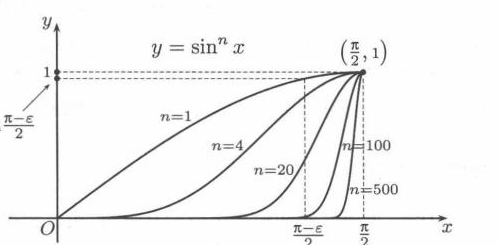
\includegraphics[width=.58\linewidth]{figures/upper/ch10/fig-10-3.png}

  图 10.3
\end{center}

从图中可以看出，由于 $\sin\frac\pi2=1$，因此对每个 $n$，当 $x$ 与 $\frac\pi2$ 充分接近时，函数值 $\sin^n x$ 一定接近 1。另一方面，对于固定的 $x$ 值，只要 $x$ 小于 $\frac\pi2$，则当 $n$ 增加时函数值 $\sin^n x$ 就很快趋于 0。这就是下面的“分而治之”方法的几何背景。

按照数列极限的 $\varepsilon$-$N$ 定义写出证明。对于给定的 $\varepsilon>0$，不妨设 $\varepsilon<\pi$，可以将积分分拆如下（参看图 10.3）：
\begin{align}
  0\leqslant\int_0^{\pi/2}\sin^n x\,\dd x
  &=\int_0^{(\pi-\varepsilon)/2}\sin^n x\,\dd x
    +\int_{(\pi-\varepsilon)/2}^{\pi/2}\sin^n x\,\dd x \notag\\
  &<\frac\pi2\sin^n\frac{\pi-\varepsilon}{2}+\frac\varepsilon2.
  \tag{10.8}
  \label{eq:10.8}
\end{align}
由 $0<\sin\frac{\pi-\varepsilon}{2}<1$，可见
\[
  \lim_{n\to\infty}\sin^n\frac{\pi-\varepsilon}{2}=0.
\]
从而对上述 $\varepsilon$，$\exists N$，使 $n>N$ 时，成立
\[
  0<\frac\pi2\sin^n\frac{\pi-\varepsilon}{2}<\frac\varepsilon2.
\]
因此 $n>N$ 时，就有
\[
  0\leqslant\int_0^{\pi/2}\sin^n x\,\dd x<\varepsilon.
\]
\end{xsolution}

\begin{xremark}
利用上、下极限工具（见 §3.6），还可将证明写得简洁一些。在 \eqref{eq:10.8} 的不等式中直接令 $n\to\infty$，就得到
\[
  0\leqslant\liminf_{n\to\infty}\int_0^{\pi/2}\sin^n x\,\dd x
  \leqslant\limsup_{n\to\infty}\int_0^{\pi/2}\sin^n x\,\dd x
  \leqslant\frac\varepsilon2.
\]
利用 $\varepsilon>0$ 的任意性，可见上、下极限相等且为 0。
\end{xremark}

\begin{xremark}
在分拆积分时可以采取动态方法，例如在 [41] 中按照区间
\[
  \left[0,\frac\pi2-\frac1{\sqrt[3]{n}}\right]
  \quad\text{和}\quad
  \left[\frac\pi2-\frac1{\sqrt[3]{n}},\frac\pi2\right]
\]
拆成两个积分，然后分别证明它们（作为数列）当 $n\to\infty$ 时的极限都是 0。读者可以一试。
\end{xremark}

\begin{xremark}
本题的常见错误如下：

\textbf{证}\quad 由积分第一中值定理，$\exists\xi\in(0,\frac\pi2)$，使得
\[
  \int_0^{\pi/2}\sin^n x\,\dd x
  =\sin^n\xi\int_0^{\pi/2}\dd x
  =\frac\pi2\sin^n\xi.
\]
不难看出一定有 $0<\sin\xi<1$ 成立，因此得到
\[
  \lim_{n\to\infty}\int_0^{\pi/2}\sin^n x\,\dd x
  =\lim_{n\to\infty}\frac\pi2\sin^n\xi=0.
\]

\textbf{错误分析}\quad 错误在于 $\xi$ 不是常数，而是随着 $n$ 的变化而变化的，应该记为 $\xi_n$。当 $n\to\infty$ 时，不难证明有 $\xi_n\to\frac\pi2$，因此 $\sin^n\xi_n$ 是 $1^\infty$ 型的不定式。回忆数列极限的内容，我们知道，从一个数列 $\{a_n\}$ 的每一项满足 $0<a_n<1$ 是得不出 $\lim_{n\to\infty}a_n^n=0$ 的（试举例）。
\end{xremark}

下一题是例题 2.2.3 在积分学中的推广。

\begin{xexample}[10.2.5]
设非负函数 $f\in C[a,b]$，证明：
\begin{equation}
  \lim_{n\to\infty}\left(\int_a^b f^n(x)\,\dd x\right)^{1/n}
  =\max\{f(x)\mid x\in[a,b]\}.
  \tag{10.9}
  \label{eq:10.9}
\end{equation}
\end{xexample}
\begin{xsolution}
\textbf{分析}\quad 设 $M=\max\{f(x)\mid x\in[a,b]\}$。由于 $M=0$ 时等式显然成立，因此只要考虑 $M>0$。利用熟知的极限 $\lim_{n\to\infty}\sqrt[n]{a}=1$（$a>0$），可见若存在区间 $[\alpha,\beta]\subset[a,b]$，使在这个区间上有
\begin{equation}
  f(x)\geqslant M,
  \tag{10.10}
  \label{eq:10.10}
\end{equation}
那么由
\[
  \left(\int_a^b f^n(x)\,\dd x\right)^{1/n}
  \geqslant\left(\int_\alpha^\beta f^n(x)\,\dd x\right)^{1/n}
  \geqslant M(\beta-\alpha)^{1/n}\to M\quad(n\to\infty),
\]
问题便解决了。但 $M$ 是函数 $f$ 的最大值，因此一般来说 \eqref{eq:10.10} 不可能成立。现在我们退而求其次，对 $0<\varepsilon<M$，将 \eqref{eq:10.10} 中的 $M$ 改为 $M-\varepsilon$ 则不难实现。下面就是将这个证法写出来而已。

如果 $f(x)\equiv0$，则所证等式显然成立。否则，设 $M=\max\{f(x)\mid x\in[a,b]\}$，则 $M>0$。

对 $0<\varepsilon<M$，$\exists[\alpha,\beta]\subseteq[a,b]$，使得
\[
  M-\varepsilon\leqslant f(x)\leqslant M,
  \qquad x\in[\alpha,\beta].
\]
于是有
\[
  \left(\int_a^b f^n(x)\,\dd x\right)^{1/n}
  \geqslant\left(\int_\alpha^\beta f^n(x)\,\dd x\right)^{1/n}
  \geqslant(M-\varepsilon)(\beta-\alpha)^{1/n}.
\]
对于不等式
\[
  M(b-a)^{1/n}\geqslant\left(\int_a^b f^n(x)\,\dd x\right)^{1/n}
  \geqslant(M-\varepsilon)(\beta-\alpha)^{1/n},
\]
利用上、下极限工具就得到
\[
  M\geqslant\limsup_{n\to\infty}\left(\int_a^b f^n(x)\,\dd x\right)^{1/n}
  \geqslant\liminf_{n\to\infty}\left(\int_a^b f^n(x)\,\dd x\right)^{1/n}
  \geqslant M-\varepsilon.
\]
从 $\varepsilon$ 的任意性可见上、下极限相等且等于 $M$。
\end{xsolution}

对含有参数的积分求极限的例题很多。下面的 Riemann 引理是研究 Fourier（傅里叶）级数的基本工具，其证明在一般教科书中都可找到。

\begin{xexample}[10.2.6（Riemann 引理）]
设 $f\in R[a,b]$，则
\[
  \lim_{p\to+\infty}\int_a^b f(x)\sin px\,\dd x=0,
  \qquad
  \lim_{p\to+\infty}\int_a^b f(x)\cos px\,\dd x=0.
\]
\end{xexample}

这个结论可以推广为

\begin{xexample}[10.2.7（Riemann 定理）]
设 $f\in R[a,b]$，$g$ 以 $T$ 为周期且在 $[0,T]$ 上可积，则
\[
  \lim_{p\to+\infty}\int_a^b f(x)g(px)\,\dd x
  =\frac1T\int_0^T g(x)\,\dd x\int_a^b f(x)\,\dd x.
\]
\end{xexample}

其证明留作为本章的第二组参考题 4。需要指出，以上两个结果对于（第十二章中的）广义可积函数 $f$ 也是成立的，但这时要求 $f$ 还是绝对可积的。

\subsection{练习题}

\begin{xexercise}[1]
设 $f\in C[a,b]$，且对满足条件 $g(a)=g(b)=0$ 的每个函数 $g\in C[a,b]$，都有
\[
  \int_a^b f(x)g(x)\,\dd x=0,
\]
证明：$f\equiv0$。
\end{xexercise}
\begin{xsolution}
取
\[
  g(x)=(x-a)(b-x)f(x).
\]
则 $g\in C[a,b]$ 且 $g(a)=g(b)=0$。由题设
\[
  0=\int_a^b f(x)g(x)\,\dd x
  =\int_a^b(x-a)(b-x)f^2(x)\,\dd x.
\]
被积函数在 $[a,b]$ 上连续且非负，所以它处处为 $0$。在 $x\in(a,b)$ 上有 $(x-a)(b-x)>0$，故 $f(x)=0$。再由连续性得 $f(a)=f(b)=0$。因此
\[
  f\equiv0.
\]
\end{xsolution}


\begin{xexercise}[2]
设非负函数 $f\in R[a,b]$，且 $\int_a^b f>0$，若有多项式 $P$ 使
\[
  \int_a^b P^2(x)f(x)\,\dd x=0,
\]
证明：$P\equiv0$。
\end{xexercise}
\begin{xsolution}
反设 $P\not\equiv0$。由 $f\geqslant0$ 且 $\int_a^b f>0$，例题 10.2.1 保证存在子区间 $[c,d]\subseteq[a,b]$ 与 $\mu>0$，使
\[
  f(x)\geqslant\mu\qquad(x\in[c,d]).
\]
非零多项式只有有限个零点，故可在 $(c,d)$ 中取一个更小的闭区间 $[c_1,d_1]$，其中 $P$ 无零点。由连续性存在 $\nu>0$，使
\[
  P^2(x)\geqslant\nu\qquad(x\in[c_1,d_1]).
\]
于是
\[
  \int_a^bP^2(x)f(x)\,\dd x
  \geqslant\int_{c_1}^{d_1}P^2(x)f(x)\,\dd x
  \geqslant\mu\nu(d_1-c_1)>0,
\]
与题设矛盾。因此只能有 $P\equiv0$。
\end{xsolution}


\begin{xexercise}[3]
设 $f\in C[-1,1]$，且对 $[-1,1]$ 上的每个可积偶函数 $g$ 都有
\[
  \int_{-1}^1 f(x)g(x)\,\dd x=0,
\]
证明：$f$ 是 $[-1,1]$ 上的奇函数。
\end{xexercise}
\begin{xsolution}
令
\[
  h(x)=f(x)+f(-x).
\]
则 $h$ 是 $[-1,1]$ 上的连续偶函数，因此可在题设中取 $g=h$，得到
\[
  \int_{-1}^1 f(x)h(x)\,\dd x=0.
\]
把积分作代换 $x\mapsto-x$，又有
\[
  \int_{-1}^1 f(-x)h(x)\,\dd x=0.
\]
两式相加：
\[
  \int_{-1}^1 h^2(x)\,\dd x=0.
\]
连续非负函数积分为零只能处处为零，故
\[
  h(x)=f(x)+f(-x)\equiv0.
\]
因此 $f(-x)=-f(x)$，即 $f$ 为奇函数。
\end{xsolution}


\begin{xexercise}[4]
计算极限
\[
  \lim_{n\to\infty}\int_0^1(1-x^2)^n\,\dd x.
\]
\end{xexercise}
\begin{xsolution}
极限为 $0$。任取 $0<\delta<1$，分拆积分：
\[
  0\leqslant\int_0^1(1-x^2)^n\,\dd x
  \leqslant
  \int_0^\delta1\,\dd x+
  \int_\delta^1(1-\delta^2)^n\,\dd x.
\]
所以
\[
  0\leqslant\int_0^1(1-x^2)^n\,\dd x
  \leqslant\delta+(1-\delta)(1-\delta^2)^n.
\]
先令 $n\to\infty$，得上极限不超过 $\delta$；再令 $\delta\to0+$，即得
\[
  \boxed{\lim_{n\to\infty}\int_0^1(1-x^2)^n\,\dd x=0}.
\]
\end{xsolution}


\begin{xexercise}[5]
分析例题 10.2.4 的条件和证明过程，试写出它的可能推广，并作出证明。

（这是一道开放题，要求设计出一定的条件，使 $\lim_{n\to\infty}\int_a^b f^n(x)\,\dd x=0$ 成立。）
\end{xexercise}
\begin{xsolution}
给出一个自然的推广如下：设 $f\in C[a,b]$，满足
\[
  0\leqslant f(x)\leqslant1,
\]
且集合
\[
  E=\{x\in[a,b]\mid f(x)=1\}
\]
为零测度集，则
\[
  \lim_{n\to\infty}\int_a^b f^n(x)\,\dd x=0.
\]

证明如下。给定 $\varepsilon>0$，可用有限个开区间覆盖紧集 $E$，并使这些区间与 $[a,b]$ 的交的总长度小于 $\varepsilon/2$。把这些开区间的并记为 $U$。紧集
\[
  K=[a,b]\setminus U
\]
与 $E$ 不交，因此由连续性存在 $q<1$，使
\[
  f(x)\leqslant q\qquad(x\in K).
\]
于是
\[
  0\leqslant\int_a^b f^n(x)\,\dd x
  \leqslant\frac\varepsilon2+(b-a)q^n.
\]
当 $n$ 充分大时第二项小于 $\varepsilon/2$，故积分小于 $\varepsilon$。于是极限为 $0$。

例题 10.2.4 对应 $f(x)=\sin x$、$[a,b]=[0,\pi/2]$；这时 $f=1$ 只发生在端点 $\pi/2$，故满足上述条件。
\end{xsolution}


\begin{xexercise}[6]
已知 $x_n\in[0,\frac\pi2]$，$n=1,2,\cdots$，且满足
\[
  \frac2\pi\int_0^{\pi/2}\sin^n x\,\dd x=\sin^n x_n,
\]
计算极限 $\lim_{n\to\infty}x_n$。
\end{xexercise}
\begin{xsolution}
\textbf{解 1}\quad 由题设
\[
  \sin^n x_n=\frac2\pi I_n,
  \qquad
  I_n:=\int_0^{\pi/2}\sin^n x\,\dd x.
\]
先给出 $I_n$ 的一个不呈指数衰减的下界。对充分大的 $n$，在
\[
  x\in\left[\frac\pi2-\frac1{\sqrt n},\frac\pi2\right]
\]
上写 $y=\frac\pi2-x$，则 $0\leqslant y\leqslant1/\sqrt n$，且
\[
  \sin x=\cos y\geqslant1-\frac{y^2}{2}
  \geqslant1-\frac1{2n}.
\]
因此
\[
  I_n\geqslant\frac1{\sqrt n}
  \left(1-\frac1{2n}\right)^n.
\]
右边括号的 $n$ 次方趋于 $\ee^{-1/2}>0$，故存在 $c>0$，使充分大的 $n$ 有
\[
  \sin^n x_n=\frac2\pi I_n\geqslant\frac{c}{\sqrt n}.
\]

若 $x_n$ 不趋于 $\pi/2$，则存在 $\delta>0$ 与子列 $n_k$，使
\[
  x_{n_k}\leqslant\frac\pi2-\delta.
\]
令 $q=\sin(\frac\pi2-\delta)<1$，则
\[
  \sin^{n_k}x_{n_k}\leqslant q^{n_k},
\]
而 $q^{n_k}$ 比 $n_k^{-1/2}$ 衰减快，和上面的下界矛盾。因此
\[
  \boxed{\lim_{n\to\infty}x_n=\frac\pi2}.
\]

\textbf{另解}\quad 记
\[
  I_n=\int_0^{\pi/2}\sin^n x\,\dd x.
\]
题设给出
\[
  \sin x_n=\left(\frac2\pi I_n\right)^{1/n}
  =\left(\frac2\pi\right)^{1/n}I_n^{1/n}.
\]
由例题 10.2.5 对 $f(x)=\sin x$ 的结论，
\[
  \lim_{n\to\infty}I_n^{1/n}
  =\max_{0\leqslant x\leqslant\pi/2}\sin x=1,
\]
而 $(2/\pi)^{1/n}\to1$，故 $\sin x_n\to1$。因为 $x_n\in[0,\pi/2]$ 且 $\sin x$ 在该区间严格增加，遂有
\[
  \boxed{\lim_{n\to\infty}x_n=\frac\pi2}.
\]
\end{xsolution}


\begin{xexercise}[7]
设 $f\in C[-1,1]$，证明：
\[
  \lim_{h\to0+}\int_{-1}^1\frac{h}{h^2+x^2}f(x)\,\dd x=\pi f(0).
\]
\end{xexercise}
\begin{xsolution}
记
\[
  K_h(x)=\frac{h}{h^2+x^2},\qquad h>0.
\]
把积分写为
\[
  \int_{-1}^1K_h(x)f(x)\,\dd x
  =f(0)\int_{-1}^1K_h(x)\,\dd x
  +\int_{-1}^1K_h(x)(f(x)-f(0))\,\dd x.
\]
第一项中
\[
  \int_{-1}^1K_h(x)\,\dd x
  =2\arctan\frac1h\longrightarrow\pi.
\]

只需证明余项趋于 $0$。给定 $\varepsilon>0$，由 $f$ 在 $0$ 连续，取 $\delta\in(0,1)$，使 $\abs{x}<\delta$ 时
\[
  \abs{f(x)-f(0)}<\varepsilon.
\]
又令 $M=\max_{[-1,1]}\abs{f(x)-f(0)}$。则
\begin{align*}
  \abs*{\int_{-1}^1K_h(x)(f(x)-f(0))\,\dd x}
  &\leqslant
  \varepsilon\int_{-\delta}^{\delta}K_h(x)\,\dd x
  +2M\int_\delta^1\frac{h}{x^2}\,\dd x\\
  &\leqslant \pi\varepsilon+\frac{2Mh}{\delta}.
\end{align*}
先令 $h\to0+$，再令 $\varepsilon\to0+$，余项为 $0$。故
\[
  \boxed{\lim_{h\to0+}\int_{-1}^1\frac{h}{h^2+x^2}f(x)\,\dd x=\pi f(0)}.
\]
\end{xsolution}


\begin{xexercise}[8]
设 $f\in C[0,1]$，计算：
\begin{enumerate}[label=(\arabic*)]
  \item $\displaystyle\lim_{n\to\infty}\int_0^1x^nf(x)\,\dd x$；
  \item $\displaystyle\lim_{n\to\infty}\int_0^1nx^nf(x)\,\dd x$。
\end{enumerate}
\end{xexercise}
\begin{xsolution}
\textbf{（1）}\quad
设 $M=\max_{[0,1]}\abs{f(x)}$，则
\[
  \abs*{\int_0^1x^nf(x)\,\dd x}
  \leqslant M\int_0^1x^n\,\dd x
  =\frac{M}{n+1}\to0.
\]
故极限为
\[
  \boxed{0}.
\]

\textbf{（2）}\quad
写成
\[
  n\int_0^1x^nf(x)\,\dd x
  =f(1)\frac{n}{n+1}
  +n\int_0^1x^n(f(x)-f(1))\,\dd x.
\]
第一项趋于 $f(1)$。对第二项，给定 $\varepsilon>0$，由 $f$ 在 $1$ 连续，可取 $\delta\in(0,1)$，使 $1-\delta<x\leqslant1$ 时
\[
  \abs{f(x)-f(1)}<\varepsilon.
\]
若 $M=\max_{[0,1]}\abs{f(x)-f(1)}$，则
\begin{align*}
  n\int_0^1x^n\abs{f(x)-f(1)}\,\dd x
  &\leqslant nM\int_0^{1-\delta}x^n\,\dd x
  +n\varepsilon\int_{1-\delta}^1x^n\,\dd x\\
  &\leqslant M(1-\delta)^{n+1}+\varepsilon.
\end{align*}
令 $n\to\infty$ 后再令 $\varepsilon\to0$，第二项趋于 $0$。因此
\[
  \boxed{\lim_{n\to\infty}\int_0^1nx^nf(x)\,\dd x=f(1)}.
\]
\end{xsolution}


\begin{xexercise}[9]
设正数列 $\{a_n\}$ 满足
\[
  \lim_{n\to\infty}\int_0^{a_n}x^n\,\dd x=2,
\]
计算极限 $\lim_{n\to\infty}a_n$。
\end{xexercise}
\begin{xsolution}
直接计算
\[
  \int_0^{a_n}x^n\,\dd x=\frac{a_n^{n+1}}{n+1}\to2.
\]
所以
\[
  a_n^{n+1}=2(n+1)(1+\littleo(1)).
\]
取对数：
\[
  (n+1)\ln a_n=\ln(n+1)+\ln2+\littleo(1).
\]
除以 $n+1$，右端趋于 $0$，故 $\ln a_n\to0$，从而
\[
  \boxed{\lim_{n\to\infty}a_n=1}.
\]
\end{xsolution}


\begin{xexercise}[10]
设 $n\in\NN_+$，
\[
  I_n=\int_0^{\pi/2}\frac{\sin^2nt}{\sin t}\,\dd t,
\]
计算极限 $\displaystyle\lim_{n\to\infty}\frac{I_n}{\ln n}$。
\end{xexercise}
\begin{xsolution}
记
\[
  I_n=\int_0^{\pi/2}\frac{\sin^2nt}{\sin t}\,\dd t.
\]
利用恒等式
\[
  \sin^2nt-\sin^2(n-1)t
  =\sin( (2n-1)t)\sin t,
\]
得到
\begin{align*}
  I_n-I_{n-1}
  &=\int_0^{\pi/2}\sin((2n-1)t)\,\dd t\\
  &=\frac1{2n-1}.
\end{align*}
并且 $I_1=1$，所以
\[
  I_n=\sum_{k=1}^n\frac1{2k-1}
  =H_{2n}-\frac12H_n,
\]
其中 $H_n=\sum_{k=1}^n1/k$。由 $H_n=\ln n+\bigO(1)$，
\[
  I_n=\frac12\ln n+\bigO(1).
\]
因此
\[
  \boxed{\lim_{n\to\infty}\frac{I_n}{\ln n}=\frac12}.
\]
\end{xsolution}


\section{变限积分与微积分基本定理}

本节的例题和练习题以变限积分方法为中心，而将以 Newton-Leibniz 公式为主的内容放在下一节中。

\subsection{主要命题}

关于变限积分的主要结果是下面两个命题。

\begin{xtheorem}[10.3.1]
设 $f\in R[a,b]$，则变上限积分 $\int_a^x f(t)\,\dd t$ 与变下限积分 $\int_x^b f(t)\,\dd t$ 都是 $[a,b]$ 上的连续函数。
\end{xtheorem}

\begin{xtheorem}[10.3.2]
设 $f\in R[a,b]$，$x\in[a,b]$ 是 $f$ 的连续点，则
\[
  \frac{\dd}{\dd x}\int_a^x f(t)\,\dd t=f(x).
\]
\end{xtheorem}

由此就给出了原函数存在的一个充分条件。

\begin{xtheorem}[10.3.3（原函数存在定理）]
设 $f\in C[a,b]$，则 $f$ 在 $[a,b]$ 上存在原函数。
\end{xtheorem}

\begin{xtheorem}[10.3.4（微积分基本公式）]
设 $F$ 在 $[a,b]$ 上有连续的导函数，则对每个 $x\in[a,b]$，成立 Newton-Leibniz 公式：
\[
  \int_a^x F'(t)\,\dd t=F(x)-F(a).
\]
\end{xtheorem}

在多数文献中将命题 10.3.2 和（或）命题 10.3.4 称为\textbf{微积分基本定理}。这是 Newton 和 Leibniz 发现的。在他们之前，微分和积分的许多个别结果已经得到。但是只有当 Newton 和 Leibniz 发现了微分和积分运算的互逆关系之后，微积分才成为统一的整体并开始了全新的发展（这方面可参看 [6] 和 [60] 的第三章）。

比命题 10.3.4 更一般的是

\begin{xtheorem}[10.3.5]
设 $f\in R[a,b]$，$F$ 是 $f$ 在 $[a,b]$ 上的一个原函数，则对每个 $x\in[a,b]$，成立 Newton-Leibniz 公式：
\[
  \int_a^x f(t)\,\dd t=F(x)-F(a).
\]
\end{xtheorem}

\begin{xremark}
这个命题也被称为微积分基本定理，但是它的证明完全不需要关于变上限积分的命题。此外，两个条件缺一不可。关于这些问题有许多深入的研究，例如可以参考 [57] 以及其中所引的文献。
\end{xremark}

\begin{xremark}
命题 10.3.5 可推广如下。设 $f\in R[a,b]$，$F\in C[a,b]$，且除了有限个点之外满足条件 $F'=f$，则对于每个 $x\in[a,b]$，仍成立等式
\[
  \int_a^x f(t)\,\dd t=F(x)-F(a),
\]
这有时称为广义的 Newton-Leibniz 公式。

例如有
\[
  \int_{-1}^3\operatorname{sgn}x\,\dd x=\abs{x}\Big|_{-1}^3=2.
\]
\end{xremark}

\begin{xthought}
举例：（1）可积函数未必有原函数；（2）有原函数的函数未必可积。
\end{xthought}
\begin{xsolution}
可取
\[
  f(x)=\operatorname{sgn}x,\qquad x\in[-1,1],
\]
并任意补定 $f(0)$。该函数只有一个跳跃间断点，所以 Riemann 可积；但导函数具有 Darboux 性质，而 $\operatorname{sgn}x$ 在 $0$ 两侧分别取负值与正值，却不具有介值性，因此它不可能是任何函数的导函数，即没有原函数。

令
\[
  F(x)=
  \begin{cases}
    x^2\sin\dfrac1{x^2},&x\ne0,\\
    0,&x=0.
  \end{cases}
\]
则 $F$ 在 $[-1,1]$ 上处处可导，且
\[
  F'(0)=0,
\]
而当 $x\ne0$ 时
\[
  F'(x)=2x\sin\frac1{x^2}-\frac2x\cos\frac1{x^2}.
\]
第二项在 $x\to0$ 时无界，因此导函数 $F'$ 在 $[-1,1]$ 上无界。Riemann 可积函数必有界，所以 $F'$ 有原函数 $F$，但 $F'$ 不可积。
\end{xsolution}


\begin{xremark}
由于有第一类间断点的函数不能是导函数，因此（1）是容易的。对于（2），可以考虑在区间 $[-1,1]$ 上的下列函数的导函数是否可积：
\[
  f(x)=
  \begin{cases}
    x^2\sin\dfrac1{x^2},&x\ne0,\\
    0,&x=0.
  \end{cases}
\]
\end{xremark}

\subsection{例题}

在命题 10.3.1 中出现的变限积分不仅在建立微积分基本定理时有用，而且是一种非常有效的工具。对于 $f\in C[a,b]$，引入变限积分
\[
  F(x)=\int_a^x f(t)\,\dd t,
\]
则 $F(x)$ 为 $[a,b]$ 上的连续可微函数。因此，我们就有可能同时用微分学和积分学的工具去研究它。

下一题的证明和应用一般出现在二重积分理论中，但在这里用变限积分方法来证明还是很容易的。

\begin{xexample}[10.3.1]
设 $f\in C[0,+\infty)$，$a>0$，证明：
\[
  \int_0^a\left(\int_0^x f(t)\,\dd t\right)\dd x
  =\int_0^a f(x)(a-x)\,\dd x.
\]
\end{xexample}
\begin{xsolution}
将 $a$ 看成非负变量，等式两边就成为变上限积分。当 $a=0$ 时两边都等于 0，然后将两边对 $a$ 求导。右边求导后得到
\[
  \left(\int_0^a f(x)(a-x)\,\dd x\right)'
  =\left(a\int_0^a f(x)\,\dd x-\int_0^a xf(x)\,\dd x\right)'
  =\int_0^a f(x)\,\dd x,
\]
与左边求导结果相同，从 Newton-Leibniz 公式就得到所求的等式。
\end{xsolution}

下一题虽然不难，但很容易出错。先看正确的做法。

\begin{xexample}[10.3.2]
设 $f\in R[A,B]$，$a,b\in(A,B)$ 是 $f$ 的两个连续点，证明：
\[
  \lim_{h\to0}\int_a^b\frac{f(x+h)-f(x)}{h}\,\dd x=f(b)-f(a).
\]
\end{xexample}
\begin{xsolution}
要点是利用变量代换改变积分界限，然后利用命题 10.3.2 计算如下：
\begin{align*}
  \lim_{h\to0}\int_a^b\frac{f(x+h)-f(x)}h\,\dd x
  &=\lim_{h\to0}\frac1h\left(\int_a^b f(x+h)\,\dd x-\int_a^b f(x)\,\dd x\right)\\
  &=\lim_{h\to0}\frac1h\left(\int_{a+h}^{b+h}f(x)\,\dd x-\int_a^b f(x)\,\dd x\right)\\
  &=\lim_{h\to0}\frac1h\left(\int_b^{b+h}f(x)\,\dd x-\int_a^{a+h}f(x)\,\dd x\right)\\
  &=f(b)-f(a).
\end{align*}
\end{xsolution}

\begin{xremark}
\textbf{错误证法分析}\quad 下面的“证法”是很有诱惑力的：
\[
  \lim_{h\to0}\int_a^b\frac{f(x+h)-f(x)}h\,\dd x
  =\int_a^b\lim_{h\to0}\frac{f(x+h)-f(x)}h\,\dd x
  =\int_a^b f'(x)\,\dd x=f(b)-f(a).
\]
请初学者注意：上面的三步推导中的每一步都是错误的，即犯了三个错误：（1）没有根据就将求极限与求积分运算交换顺序；（2）对差商求极限时忘记了题中 $f$ 只在两点连续，并无可导条件；（3）即使 $f$ 在 $[a,b]$ 上可导，但导函数也不一定可积，因此不能用 Newton-Leibniz 公式。
\end{xremark}

下一题的第一个证明是引进变限积分方法的典型应用。

\begin{xexample}[10.3.3]
设 $f\in C[a,b]$，且满足条件
\[
  \int_a^b x^k f(x)\,\dd x=0\qquad(k=0,1,\cdots,n),
\]
证明：函数 $f$ 在 $(a,b)$ 内至少有 $n+1$ 个不同的零点。
\end{xexample}
\begin{xsolution}
\textbf{证 1}\quad 用数学归纳法。对于 $n=0$，从 $\int_a^b f(x)\,\dd x=0$ 和 $f\in C[a,b]$ 可见 $f$ 在 $(a,b)$ 上或变号，或恒等于 0，因此至少有一个零点。

设对于 $n$ 的结论已成立，我们讨论 $n+1$ 的情况。引入辅助函数
\[
  F(x)=\int_a^x f(t)\,\dd t,
\]
这时 $F(a)=0$。从 $f$ 满足的条件 $\int_a^b f(x)\,\dd x=0$ 得到 $F(b)=0$。又从分部积分可见对 $k\geqslant1$ 有
\begin{align*}
  \int_a^b x^k f(x)\,\dd x
  &=\int_a^b x^k\,\dd F(x)
  =x^kF(x)\Big|_a^b-\int_a^b kx^{k-1}F(x)\,\dd x\\
  &=-\int_a^b kx^{k-1}F(x)\,\dd x,
\end{align*}
因此有
\[
  \int_a^b x^k f(x)\,\dd x=0
  \Longrightarrow
  \int_a^b x^{k-1}F(x)\,\dd x=0,
  \qquad k=1,\cdots,n+1.
\]
根据归纳假设，$F$ 在 $(a,b)$ 内至少有 $n+1$ 个零点。将它们记为 $x_1<x_2<\cdots<x_{n+1}$。由于 $a$ 和 $b$ 又都是 $F$ 的零点，改记 $a=x_0$，$b=x_{n+2}$，并对 $[x_i,x_{i+1}]$，$i=0,1,\cdots,n+1$，用 $n+2$ 次 Rolle 定理，就得到所要求的 $n+2$ 个零点。

下面再给出不利用变限积分的一个证明。

\textbf{证 2}\quad 用反证法：设有一个 $f$ 满足所有题设条件，但其零点个数不超过 $n$。这时 $f$ 在 $[a,b]$ 内的任何闭子区间上不会恒等于 0，因此从条件 $\int_a^b f(x)\,\dd x=0$ 可见 $f$ 在区间 $[a,b]$ 上一定变号。

利用 $f$ 的所有零点或其中的一部分，可以作出区间 $[a,b]$ 的一个分割
\[
  P=\{x_0,x_1,\cdots,x_k\},
\]
其中 $x_0=a$，$x_k=b$，中间的 $k-1$ 个分点都是 $f$ 的零点，$f$ 在每个子区间上不变号，而在相邻的子区间上 $f$ 的符号相反。

由反证法前提可见 $k-1\leqslant n$。

对于分割 $P$ 可以构造辅助多项式
\[
  g(x)=(x-x_1)(x-x_2)\cdots(x-x_{k-1}).
\]
$g$ 关于分割 $P$ 具有与 $f$ 相同的性质：即在每个子区间上不变号，而在相邻的子区间上符号相反。这样就知道 $f\cdot g$ 在整个区间 $[a,b]$ 上不变号，因此
\[
  \int_a^b f(x)g(x)\,\dd x>0\quad(<0).
\]
另一方面，由于 $g$ 是次数不超过 $n$ 的多项式，从题设条件可见上述积分应当等于 0，从而引出矛盾。
\end{xsolution}

\subsection{练习题}

\begin{xexercise}[1]
计算下列各题：
\begin{enumerate}[label=(\arabic*)]
  \item $\displaystyle\left(\int_0^x t\sin\frac1t\,\dd t\right)'\Big|_{x=0}$；
  \item $\displaystyle\frac{\dd}{\dd x}\int_{x^2}^{x^3}\frac{\sin t}{t}\,\dd t$；
  \item $\displaystyle\lim_{x\to0}\frac{\int_0^x(\arctan t)^2\,\dd t}{x^2}$；
  \item $\displaystyle\lim_{x\to+\infty}\frac{\left(\int_0^x\ee^{t^2}\,\dd t\right)^2}{\int_0^x\ee^{2t^2}\,\dd t}$。
\end{enumerate}
\end{xexercise}
\begin{xsolution}
\textbf{（1）}\quad
令
\[
  G(x)=\int_0^x t\sin\frac1t\,\dd t,
\]
其中在 $t=0$ 的函数值可任意补定。由于 $G(0)=0$，
\[
  \abs*{\frac{G(x)-G(0)}x}
  \leqslant\frac1{\abs x}\int_0^{\abs x}t\,\dd t
  =\frac{\abs x}{2}\to0.
\]
故
\[
  \boxed{G'(0)=0}.
\]

\textbf{（2）}\quad
把 $\sin t/t$ 在 $t=0$ 处补定义为 $1$，得到连续函数
\[
  \varphi(t)=
  \begin{cases}
    \dfrac{\sin t}{t},&t\ne0,\\
    1,&t=0.
  \end{cases}
\]
于是由变限积分求导公式
\[
  \frac{\dd}{\dd x}\int_{x^2}^{x^3}\frac{\sin t}{t}\,\dd t
  =3x^2\varphi(x^3)-2x\varphi(x^2).
\]
因此当 $x\ne0$ 时可写为
\[
  \boxed{\frac{3\sin x^3-2\sin x^2}{x}},
\]
而在 $x=0$ 时导数为 $0$。

\textbf{（3）}\quad
这是 $0/0$ 型。由 L'Hospital 法则，
\[
  \lim_{x\to0}\frac{\int_0^x(\arctan t)^2\,\dd t}{x^2}
  =\lim_{x\to0}\frac{(\arctan x)^2}{2x}=0,
\]
因为 $\arctan x\sim x$。故极限为
\[
  \boxed{0}.
\]

\textbf{（4）}\quad
记
\[
  A(x)=\int_0^x\ee^{t^2}\,\dd t,
  \qquad
  B(x)=\int_0^x\ee^{2t^2}\,\dd t.
\]
当 $x\to+\infty$ 时二者都趋于 $+\infty$，且所求比值为 $A^2/B$。一次用 L'Hospital 法则，
\[
  \lim_{x\to+\infty}\frac{A^2(x)}{B(x)}
  =\lim_{x\to+\infty}2A(x)\ee^{-x^2}.
\]
又
\[
  \lim_{x\to+\infty}\frac{A(x)}{\ee^{x^2}}
  =\lim_{x\to+\infty}\frac{\ee^{x^2}}{2x\ee^{x^2}}
  =0.
\]
故
\[
  \boxed{\lim_{x\to+\infty}\frac{\left(\int_0^x\ee^{t^2}\,\dd t\right)^2}
  {\int_0^x\ee^{2t^2}\,\dd t}=0}.
\]
\end{xsolution}


\begin{xexercise}[2]
设 $f\in C[a,b]$，且存在常数 $M,\eta>0$，使对每个 $[\alpha,\beta]\subseteq[a,b]$，恒有
\[
  \abs*{\int_\alpha^\beta f(x)\,\dd x}\leqslant M(\beta-\alpha)^{1+\eta},
\]
证明：$f\equiv0$。
\end{xexercise}
\begin{xsolution}
任取 $x\in[a,b)$，令 $0<h\leqslant b-x$。题设给出
\[
  \abs*{\frac1h\int_x^{x+h}f(t)\,\dd t}\leqslant Mh^\eta.
\]
因为 $f$ 在 $x$ 连续，由积分第一中值定理或变限积分基本定理，
\[
  \lim_{h\to0+}\frac1h\int_x^{x+h}f(t)\,\dd t=f(x).
\]
而右边 $Mh^\eta\to0$，故 $f(x)=0$。端点 $b$ 再由连续性得到 $f(b)=0$。所以
\[
  f\equiv0.
\]
\end{xsolution}


\begin{xexercise}[3]
设 $f\in C[a,b]$，且在 $[a,b]$ 上满足不等式
\[
  f(x)\leqslant\int_a^x f(t)\,\dd t,
\]
证明：在 $[a,b]$ 上 $f(x)\leqslant0$。
\end{xexercise}
\begin{xsolution}
令
\[
  F(x)=\int_a^x f(t)\,\dd t.
\]
则 $F(a)=0$，且 $F'(x)=f(x)$。题设即
\[
  F'(x)\leqslant F(x).
\]
于是
\[
  \bigl(\ee^{-x}F(x)\bigr)'=\ee^{-x}(F'(x)-F(x))\leqslant0.
\]
所以对 $x\in[a,b]$，
\[
  \ee^{-x}F(x)\leqslant\ee^{-a}F(a)=0,
\]
即 $F(x)\leqslant0$。最后由题设 $f(x)\leqslant F(x)$，得到
\[
  \boxed{f(x)\leqslant0\quad(x\in[a,b])}.
\]
\end{xsolution}


\begin{xexercise}[4]
设函数 $f\in C[0,\pi]$，且有
\[
  \int_0^\pi f(t)\cos t\,\dd t=\int_0^\pi f(t)\sin t\,\dd t=0,
\]
证明：$f$ 在区间 $(0,\pi)$ 内至少有两个零点。
\end{xexercise}
\begin{xsolution}
先证明 $f$ 至少有一个零点。若 $f$ 在 $(0,\pi)$ 无零点，由连续性它在 $(0,\pi)$ 恒正或恒负。由于 $\sin t>0$，便有
\[
  \int_0^\pi f(t)\sin t\,\dd t\ne0,
\]
与题设矛盾。

反设 $f$ 在 $(0,\pi)$ 中恰有一个零点 $c$。由上面的正弦积分等于 $0$ 可知，$f$ 必须在 $c$ 两侧变号。函数
\[
  \varphi(t)=\sin(t-c)=\sin t\cos c-\cos t\sin c
\]
在 $(0,c)$ 与 $(c,\pi)$ 两侧也恰好异号。必要时将 $\varphi$ 乘以 $-1$，可使 $f(t)\varphi(t)\geqslant0$，并且除零点外严格大于 $0$。因此
\[
  \int_0^\pi f(t)\varphi(t)\,\dd t>0.
\]
但由题设两个正交条件，
\[
  \int_0^\pi f(t)\varphi(t)\,\dd t
  =\cos c\int_0^\pi f(t)\sin t\,\dd t
  -\sin c\int_0^\pi f(t)\cos t\,\dd t=0,
\]
矛盾。故 $f$ 在 $(0,\pi)$ 内至少有两个零点。
\end{xsolution}


\begin{xexercise}[5]
设 $f$ 为周期函数，且于每个有界区间上可积，证明：变上限积分
\[
  F(x)=\int_0^x f(t)\,\dd t
\]
可以表示为一个周期函数与一个线性函数之和。
\end{xexercise}
\begin{xsolution}
设 $T>0$ 是 $f$ 的一个周期，令
\[
  c=\frac1T\int_0^T f(t)\,\dd t,
  \qquad
  G(x)=\int_0^x(f(t)-c)\,\dd t.
\]
周期函数在任意长度为 $T$ 的区间上的积分相同，所以
\[
  \int_x^{x+T}(f(t)-c)\,\dd t
  =\int_0^T f(t)\,\dd t-cT=0.
\]
于是
\[
  G(x+T)-G(x)=0,
\]
即 $G$ 是周期为 $T$ 的周期函数。另一方面
\[
  F(x)=\int_0^x f(t)\,\dd t=G(x)+cx.
\]
故 $F$ 是一个周期函数与一个线性函数之和。
\end{xsolution}


\begin{xexercise}[6]
设 $f\in C(-\infty,+\infty)$，且积分 $\int_a^{a+T}f(x)\,\dd x$ 的值与 $a$ 无关，证明：$f$ 为周期函数。
\end{xexercise}
\begin{xsolution}
设
\[
  H(a)=\int_a^{a+T}f(x)\,\dd x.
\]
题设说明 $H$ 为常数。由于 $f$ 连续，可对变动积分限求导：
\[
  H'(a)=f(a+T)-f(a)=0.
\]
故对一切 $a\in\RR$，
\[
  f(a+T)=f(a),
\]
所以 $f$ 是周期为 $T$ 的周期函数。
\end{xsolution}


\begin{xexercise}[7]
设 $f\in C(0,+\infty)$，且对任何 $a,b>0$ 的积分 $\int_a^{ab}f(x)\,\dd x$ 的值与 $a$ 无关，试求函数 $f$。
\end{xexercise}
\begin{xsolution}
对每个固定的 $b>0$，令
\[
  H_b(a)=\int_a^{ab}f(x)\,\dd x.
\]
题设说明 $H_b(a)$ 与 $a$ 无关，所以
\[
  0=H_b'(a)=b f(ab)-f(a).
\]
于是对任意 $a,b>0$，
\[
  b f(ab)=f(a).
\]
取 $a=1$，得到
\[
  f(b)=\frac{f(1)}b.
\]
因此全部解为
\[
  \boxed{f(x)=\frac Cx\quad(x>0)},
\]
其中 $C$ 为任意常数。反过来，
\[
  \int_a^{ab}\frac Cx\,\dd x=C\ln b,
\]
确与 $a$ 无关。
\end{xsolution}


\begin{xexercise}[8]
设 $f\in R[a,b]$，证明：存在 $\xi\in[a,b]$，使成立
\[
  \int_\xi^b f(x)\,\dd x=\int_a^\xi f(x)\,\dd x,
\]
并举例说明这样的 $\xi$ 在 $(a,b)$ 内不一定存在。
\end{xexercise}
\begin{xsolution}
令
\[
  H(\xi)=\int_a^\xi f(x)\,\dd x-\int_\xi^b f(x)\,\dd x
  =2\int_a^\xi f(x)\,\dd x-\int_a^b f(x)\,\dd x.
\]
由命题 10.3.1，$H$ 连续。记 $I=\int_a^b f$，则
\[
  H(a)=-I,
  \qquad
  H(b)=I.
\]
由介值定理，存在 $\xi\in[a,b]$ 使 $H(\xi)=0$，即
\[
  \int_\xi^b f=\int_a^\xi f.
\]

这样的 $\xi$ 未必能取在开区间内。例如在 $[0,1]$ 上取
\[
  f(x)=1-2x.
\]
此时 $\int_0^1 f=0$，并且
\[
  \int_0^\xi f(x)\,\dd x=\xi-\xi^2>0
  \qquad(0<\xi<1).
\]
题中等式在总积分为 $0$ 时等价于 $\int_0^\xi f=0$，因此只有 $\xi=0,1$ 两个端点解，没有内点解。
\end{xsolution}


\begin{xexercise}[9]
设 $f\in C[a,b]$，且处处大于 0，证明：在 $[a,b]$ 上有
\[
  \frac{\dd}{\dd x}\left(\int_a^x f(t)\,\dd t-\int_x^b\frac{\dd t}{f(t)}\right)\geqslant2.
\]
\end{xexercise}
\begin{xsolution}
由 $f>0$，有
\begin{align*}
  \frac{\dd}{\dd x}
  \left(\int_a^x f(t)\,\dd t-\int_x^b\frac{\dd t}{f(t)}\right)
  &=f(x)+\frac1{f(x)}\\
  &\geqslant2,
\end{align*}
其中最后一步是正数的算术--几何平均不等式。因此题中不等式成立。
\end{xsolution}



\begin{xexercise}[10]
设 $a(t),b(t),c(t),d(t)$ 均为变量 $t$ 的多项式，证明：
\[
  \int_1^x a(t)c(t)\,\dd t\int_1^x b(t)d(t)\,\dd t
  -\int_1^x a(t)d(t)\,\dd t\int_1^x b(t)c(t)\,\dd t
\]
可被 $(x-1)^4$ 整除。
\end{xexercise}
\begin{xsolution}
记
\[
  A(x)=\int_1^x a(t)c(t)\,\dd t,\quad
  B(x)=\int_1^x b(t)d(t)\,\dd t,
\]
\[
  C(x)=\int_1^x a(t)d(t)\,\dd t,\quad
  D(x)=\int_1^x b(t)c(t)\,\dd t,
\]
并令 $E(x)=A(x)B(x)-C(x)D(x)$。由于 $a,b,c,d$ 都是多项式，$A,B,C,D,E$ 也都是多项式。

令 $h=x-1$，并简记
\[
  p=ac,\quad q=bd,\quad r=ad,\quad s=bc.
\]
在 $t=1$ 附近作 Taylor 展开，有
\[
  A(x)=p(1)h+\frac{p'(1)}2h^2+\bigO(h^3),
\]
其余三个积分同理。因此
\begin{align*}
  E(x)
  &=[p(1)q(1)-r(1)s(1)]h^2\\
  &\quad+\frac12[p'(1)q(1)+p(1)q'(1)-r'(1)s(1)-r(1)s'(1)]h^3
  +\bigO(h^4).
\end{align*}
第一项系数为
\[
  (ac)(bd)-(ad)(bc)=0.
\]
第二项括号展开为
\begin{align*}
 &(ac)'bd+ac(bd)'-(ad)'bc-ad(bc)'\\
 &=a'cbd+ac'bd+acb'd+acbd'\\
 &\quad-a'dbc-ad'bc-adb'c-adbc'=0,
\end{align*}
其中各量均取在 $t=1$，各项两两抵消。故
\[
  E(x)=\bigO((x-1)^4)\qquad(x\to1).
\]
而 $E$ 是多项式，所以 $x=1$ 是 $E$ 的至少四重零点，即
\[
  \boxed{(x-1)^4\mid E(x)}.
\]
\end{xsolution}


\begin{xexercise}[11]
设 $f\in C(-\infty,+\infty)$，$g(x)=f(x)\int_0^x f(t)\,\dd t$ 且单调减少，证明：$f=0$。
\end{xexercise}
\begin{xsolution}
令
\[
  F(x)=\int_0^x f(t)\,\dd t.
\]
则 $F'=f$，并且
\[
  g(x)=f(x)F(x)=\frac12(F^2(x))'.
\]
题设说 $g$ 单调减少，故 $(F^2)'$ 单调减少，于是 $F^2$ 是 $\RR$ 上的凹函数。

任何在整个实轴上非负的凹函数都只能是常数。事实上，若某两点 $x_1<x_2$ 有 $F^2(x_2)>F^2(x_1)$，则割线斜率为正；由凹性，向左延长时函数值最终会小于 $0$，矛盾。若 $F^2(x_2)<F^2(x_1)$，则向右延长同样得到矛盾。因此 $F^2$ 为常数。

又 $F(0)=0$，所以 $F^2\equiv0$，即 $F\equiv0$。于是
\[
  f=F'\equiv0.
\]
\end{xsolution}


\begin{xexercise}[12]
设 $f$ 在 $[0,+\infty)$ 上可微，且满足
\[
  \int_0^x t f(t)\,\dd t=\frac{x}{3}\int_0^x f(t)\,\dd t,
\]
求 $f$。
\end{xexercise}
\begin{xsolution}
令
\[
  F(x)=\int_0^x f(t)\,\dd t.
\]
题设为
\[
  \int_0^x t f(t)\,\dd t=\frac x3F(x).
\]
对 $x>0$ 求导：
\[
  x f(x)=\frac13F(x)+\frac x3 f(x),
\]
即
\[
  F(x)=2x f(x).
\]
再求导，利用 $F'=f$，得
\[
  f(x)=2f(x)+2x f'(x),
\]
故
\[
  2x f'(x)+f(x)=0.
\]
在 $(0,+\infty)$ 上其一般解为
\[
  f(x)=\frac C{\sqrt x}.
\]
但题设 $f$ 在 $[0,+\infty)$ 上可微，特别在 $0$ 连续，因此只有 $C=0$ 才可能。故
\[
  \boxed{f\equiv0}.
\]
\end{xsolution}


\section{定积分的计算}

一般来说，从定义出发来计算定积分是不切实际的。本节以 Newton-Leibniz 公式（见命题 10.3.4 和 10.3.5）为基础，在前三小节中介绍定积分计算，在最后一小节则与定积分计算相结合介绍积分中值定理的应用。（有关不等式、积分估计和近似计算等例题见下一章。）

\subsection{计算公式与法则}

与不定积分的计算法则相对应，定积分的计算法则有以下两个。

\begin{xtheorem}[10.4.1（定积分的分部积分法）]
设 $u'(x),v'(x)\in R[a,b]$，则
\begin{equation}
  \int_a^b u(x)\,\dd v(x)
  =u(x)v(x)\Big|_a^b-\int_a^b v(x)\,\dd u(x).
  \tag{10.11}
  \label{eq:10.11}
\end{equation}
\end{xtheorem}

\begin{xremark}
在应用上述公式时，如果 $u(a)v(a)$ 或 $u(b)v(b)$ 不存在，或者 $u(x)v(x)$ 在点 $x=a$ 或 $x=b$ 不连续，则应当将公式右边的第一项 $u(x)v(x)|_a^b$ 理解为
\[
  \lim_{x\to b-}u(x)v(x)-\lim_{x\to a+}u(x)v(x).
\]
（虽然这时 $u'(x),v'(x)$ 在点 $x=a$ 或 $x=b$ 可能不存在，但是由于函数在一个区间上的可积性以及积分值与其在有限点处的定义无关，因此这不会影响 $u'(x),v'(x)$ 的可积性以及积分值。）
\end{xremark}

\begin{xtheorem}[10.4.2（定积分的换元积分法）]
设 $f\in R[a,b]$，$x=g(t)$ 在 $[\alpha,\beta]$ 上严格单调增加，$g'(t)$ 在 $[\alpha,\beta]$ 上可积，且满足 $g(\alpha)=a$，$g(\beta)=b$，则
\[
  \int_a^b f(x)\,\dd x=\int_\alpha^\beta f(g(t))g'(t)\,\dd t.
\]
\end{xtheorem}

\begin{xremark}
如果 $f\in C[a,b]$，则 $g$ 的单调性条件可换为较弱的条件 $g([\alpha,\beta])\subseteq[a,b]$。两种情况的证明均可见 [59] 第二册 140 页的命题 6.1 和 6.2 及其注。
\end{xremark}

\begin{xremark}
尽管定积分的换元积分法与不定积分的相应法则在形式上是类似的，但两者还是有区别的，不能把前者简单地看成为后者与 Newton-Leibniz 公式的结合。两者的主要区别在于：定积分的计算与积分区间紧密关联，不仅换元以后积分限要作相应的改变，而且在采用变换前必须考虑进行变换所需的条件在有关区间上是否满足。相对来说，应用不定积分的换元法时对此不必多作强调，只有当需要写出原函数时才会与区间联系起来。

从下面的很多例子中可以看到，对定积分用换元法和分部积分法时往往能使一些积分项相互抵消，因此有时即使被积函数的原函数不是初等函数，我们仍然有可能计算出定积分的值。因此，定积分计算并不要求被积函数的原函数一定是初等函数，这与不定积分计算完全不同。
\end{xremark}

\subsection{例题}

\begin{xexample}[10.4.1]
计算
\[
  I=\int_0^{\pi/2}\sin x\ln\sin x\,\dd x.
\]
\end{xexample}
\begin{xsolution}
\textbf{解 1}\quad 被积函数在 $x=0$ 时没有定义，但是从 $\sin x\sim x$（$x\to0+$）和 $x\ln x\to0$（$x\to0+$）可以知道被积函数在 $x=0$ 右侧有界。

如果如下分部积分，则有
\[
  I=\int_0^{\pi/2}\ln\sin x\,\dd(-\cos x)
  =-\cos x\ln\sin x\Big|_{0+}^{\pi/2}
  +\int_0^{\pi/2}\cos x\,\dd\ln\sin x.
\]
由于右边第一项为无穷大，因此不能解决问题。克服这个困难的方法也很简单，只要将上面的 $\dd(-\cos x)$ 改为 $\dd(1-\cos x)$ 即可。利用 $1-\cos x\sim\frac12x^2$（$x\to0$），就可计算如下：
\begin{align*}
  I&=\int_0^{\pi/2}\ln\sin x\,\dd(1-\cos x)\\
   &=(1-\cos x)\ln\sin x\Big|_{0+}^{\pi/2}
    -\int_0^{\pi/2}(1-\cos x)\,\dd(\ln\sin x)\\
   &=-\int_0^{\pi/2}(1-\cos x)\frac{\cos x}{\sin x}\,\dd x
    =-\int_0^{\pi/2}\frac{\sin x\cos x}{1+\cos x}\,\dd x\\
   &=\int_0^{\pi/2}\left(-\sin x+\frac{\sin x}{1+\cos x}\right)\dd x\\
   &=[\cos x-\ln(1+\cos x)]_0^{\pi/2}=\ln2-1.
\end{align*}

\textbf{解 2}\quad 从作代换 $x=2t$ 开始可计算如下
\begin{align*}
  \int_0^{\pi/2}\sin x\ln\sin x\,\dd x
  &=\int_0^{\pi/4}2\sin2t\ln\sin2t\,\dd t\\
  &=2\ln2\int_0^{\pi/4}\sin2t\,\dd t
    +\int_0^{\pi/4}2\sin2t\ln\sin t\,\dd t
    +\int_0^{\pi/4}2\sin2t\ln\cos t\,\dd t.
\end{align*}
（对第一个积分作代换 $2t=x$，对最后一个积分作代换 $s=\frac\pi2-t$）
\begin{align*}
  &=\ln2+\int_0^{\pi/4}2\sin2t\ln\sin t\,\dd t
    +\int_{\pi/4}^{\pi/2}2\sin2s\ln\sin s\,\dd s\\
  &=\ln2+\int_0^{\pi/2}4\sin t\cos t\ln\sin t\,\dd t
\end{align*}
（利用定积分与积分变量无关的特点合并两个积分）
\begin{align*}
  &=\ln2+\int_0^1 4u\ln u\,\dd u\\
  &=\ln2+2u^2\ln u\Big|_{0+}^1-\int_0^1 2u\,\dd u
   =\ln2-1.
\end{align*}
（对积分再作代换 $\sin t=u$）
\end{xsolution}

\begin{xremark}
本题解 1 中处理分部积分的方法具有普遍意义，因此要再强调一下。具体来说，由于两个不同的原函数之间只差一个常值函数，因此在分部积分公式 \eqref{eq:10.11} 中左边的 $u(x)\,\dd v(x)$ 可改为 $u(x)\,\dd(v(x)+c)$，其中 $c$ 待定。利用这一点灵活性可以解决不少问题。
\end{xremark}

\begin{xremark}
有的文献将本题与广义积分中的 Euler 积分 $\int_0^{\pi/2}\ln\sin x\,\dd x$（见例题 12.3.4）相联系。实际上本题是常义积分，且有初等原函数，这与 Euler 积分的情况并不相同。但是本题的解 2 确实与例题 12.3.4 的解 2 中的方法类似。
\end{xremark}

下面是一个简单的题，但其中还是有不少知识点需要注意。

\begin{xexample}[10.4.2]
设 $n$ 为大于 1 的正整数，求
\[
  \int_0^n(x-[x])\,\dd x,
\]
其中 $[x]$ 表示不超过 $x$ 的最大整数。
\end{xexample}
\begin{xsolution}
由于被积函数在积分区间上只有有限个间断点，积分的存在性没有问题。但由于这有限个间断点是跳跃间断点，被积函数在整个区间上的原函数不存在（例题 7.1.1），需分段计算积分。在区间 $[0,1]$ 上，$x-[x]$ 与函数 $f(x)=x$ 仅在点 $x=1$ 处有不同的值，因此它们的可积性和积分值相同，这样就有
\[
  \int_0^1(x-[x])\,\dd x=\int_0^1x\,\dd x=\frac12.
\]
又由于 $x-[x]$ 是周期为 1 的周期函数，它在每个长度为 1 的区间上的积分相同，所以就可以得到
\[
  \int_0^n(x-[x])\,\dd x
  =\left(\int_0^1+\int_1^2+\cdots+\int_{n-1}^n\right)(x-[x])\,\dd x
  =n\int_0^1(x-[x])\,\dd x=\frac n2.
\]
\end{xsolution}

下面的例题说明，与计算不定积分一样，熟练地掌握初等代数或三角函数的运算公式，对于定积分的计算也是十分重要的。

\begin{xexample}[10.4.3]
在区间 $(0,\pi)$ 上定义
\[
  D_n(x)=\frac{\sin\frac{(2n+1)x}{2}}{2\sin\frac x2},\qquad n\in\NN_+,
\]
计算 $\int_0^\pi D_n(x)\,\dd x$。
\end{xexample}
\begin{xsolution}
虽然 $D_n(x)$ 在 $x=0$ 时无定义，但容易证明
\[
  \lim_{x\to0+}D_n(x)=\frac{2n+1}{2},
\]
因此 $D_n(x)$ 在 $[0,\pi]$ 上可积。直接对 $D_n(x)$ 积分是困难的，我们作如下变换。利用三角恒等式
\[
  2\sin\frac x2\left(\frac12+\sum_{k=1}^n\cos kx\right)
  =\sin\frac{(2n+1)x}{2},
\]
就可以将 $D_n$ 分解如下：
\[
  D_n(x)=\frac12+\sum_{k=1}^n\cos kx.
\]
逐项积分就得到
\begin{align}
  \int_0^\pi D_n(x)\,\dd x
  &=\int_0^\pi\left(\frac12+\sum_{k=1}^n\cos kx\right)\dd x \notag\\
  &=\frac\pi2+\sum_{k=1}^n\int_0^\pi\cos kx\,\dd x=\frac\pi2.
  \tag{10.12}
  \label{eq:10.12}
\end{align}
\end{xsolution}

\begin{xremark}
这个积分有时也称为 Dirichlet 积分，其中的被积函数 $D_n$ 称为 Dirichlet 核，\eqref{eq:10.12} 又可写成
\begin{equation}
  1=\frac2\pi\int_0^\pi\frac{\sin\frac{(2n+1)x}{2}}{2\sin\frac x2}\,\dd x.
  \tag{10.13}
  \label{eq:10.13}
\end{equation}
Dirichlet 核与公式 \eqref{eq:10.13} 在积分理论与级数理论中有重要的应用。
\end{xremark}

下一题虽然是对变限积分求导，但是不能直接应用命题 10.3.2。同时它也表明，该命题只给出了变限积分可导的充分条件。变限积分在被积函数不连续点上仍有可能是可导的。

\begin{xexample}[10.4.4]
设
\[
  F(x)=\int_0^x\sin\frac1t\,\dd t,
\]
求 $F'(0)$。
\end{xexample}
\begin{xsolution}
由于 $x=0$ 是被积函数的第二类间断点，不能用对变动上限求导的方法来求 $F'(0)$，而只能按照定义来计算导数。根据定义 $F(0)=0$。而当 $x\ne0$ 时，由分部积分公式可以得到
\begin{align}
  F(x)&=\int_0^x t^2\,\dd\cos\frac1t
  =t^2\cos\frac1t\Big|_0^x-\int_0^x\cos\frac1t\,\dd(t^2)\notag\\
  &=x^2\cos\frac1x-\int_0^x2t\cos\frac1t\,\dd t.
  \tag{10.14}
  \label{eq:10.14}
\end{align}
按照导数的定义计算极限：
\[
  F'(0)=\lim_{x\to0}\frac{F(x)-F(0)}x
  =\lim_{x\to0+}x\cos\frac1x
  -\lim_{x\to0+}\frac{\int_0^x2t\cos\frac1t\,\dd t}{x}.
\]
右边的第一项极限明显为 0。第二项是 $0/0$ 的不定式，用 L'Hospital 法则就得到结果是 0。因此 $F'(0)=0$。
\end{xsolution}

\begin{xremark}
$F'(0)$ 的计算也可以如下进行：虽然函数 $2t\cos\frac1t$ 在 $t=0$ 没有定义，但是可以补充定义在该点的函数值为 0。这时 \eqref{eq:10.14} 中最后一个积分的被积函数在 $t=0$ 连续，从而可以直接用命题 10.3.2。
\end{xremark}

\subsection{对称性在定积分计算中的应用}

设积分区间关于原点对称，例如为 $[-a,a]$（$a>0$）。则容易知道，当被积函数 $f$ 是奇函数，即其图像关于原点为中心对称时，就有 $\int_{-a}^a f(x)\,\dd x=0$；而当 $f$ 为偶函数，即其图像关于 $y$ 轴为对称时，就有 $\int_{-a}^a f(x)\,\dd x=2\int_0^a f(x)\,\dd x$。

如果将以上的对称性进一步推广，则对于某些积分的计算是很有好处的。下面我们会看到利用对称性甚至可以计算出被积函数没有初等原函数的某些定积分。在举例之前先列出三个简单而有用的事实，其证明留给读者。

\begin{xtheorem}[10.4.3]
设函数 $f$ 在区间 $[a,b]$ 上可积，则成立
\[
  \int_a^b f(x)\,\dd x=\int_a^b f(a+b-x)\,\dd x,
\]
特别当积分区间为 $[0,a]$ 时则有
\[
  \int_0^a f(x)\,\dd x=\int_0^a f(a-x)\,\dd x.
\]
\end{xtheorem}

\begin{xtheorem}[10.4.4]
设函数 $f$ 在区间 $[0,a]$ 上可积，且有 $f(x)=f(a-x)$，即关于区间的中点为偶函数（也就是关于直线 $x=a/2$ 为偶函数），则成立
\[
  \int_0^a f(x)\,\dd x=2\int_0^{a/2}f(x)\,\dd x.
\]
\end{xtheorem}

\begin{xtheorem}[10.4.5]
设函数 $f$ 在区间 $[0,a]$ 上可积，且有 $f(x)=-f(a-x)$，即关于区间的中点为奇函数，则成立
\[
  I=\int_0^a f(x)\,\dd x=0.
\]
\end{xtheorem}

由于 $f(x)+f(a-x)$ 关于点 $x=a/2$ 总是偶函数，因此就可得到以下更为有力的命题，它包含了以上两个命题为其特例。

\begin{xtheorem}[10.4.6]
设函数 $f$ 在 $[0,a]$ 上可积，记 $f(x)+f(a-x)=g(x)$，则成立
\[
  \int_0^a f(x)\,\dd x=\int_0^{a/2}g(x)\,\dd x.
\]
\end{xtheorem}

下面 4 个定积分计算题是利用对称性的典型例题，它们都可以用命题 10.4.6 直接解决。

\begin{xexample}[10.4.5]
对任意两个不同的非零实数 $a,b$，计算
\[
  \int_0^\pi\frac{\cos x}{\sqrt{a^2\sin^2x+b^2\cos^2x}}\,\dd x.
\]
\end{xexample}
\begin{xsolution}
由于被积函数关于积分区间的中点 $\frac\pi2$ 为奇函数，因此用命题 10.4.5（或命题 10.4.6）即知该积分等于 0。
\end{xsolution}

\begin{xexample}[10.4.6]
计算
\[
  I=\int_0^\pi\frac{x\sin x}{1+\cos^2x}\,\dd x.
\]
\end{xexample}
\begin{xsolution}
\textbf{解 1}\quad 用命题 10.4.6 先计算
\[
  \frac{x\sin x}{1+\cos^2x}
  +\frac{(\pi-x)\sin(\pi-x)}{1+\cos^2(\pi-x)}
  =\frac{\pi\sin x}{1+\cos^2x},
\]
因此就有
\[
  I=\int_0^{\pi/2}\frac{\pi\sin x}{1+\cos^2x}\,\dd x
  =-\pi\arctan(\cos x)\Big|_0^{\pi/2}
  =\frac{\pi^2}{4}.
\]

\textbf{解 2}\quad 本题中所利用的对称性可以如下理解：由于被积函数 $f$ 中除去因子 $x$ 后的部分关于直线 $x=\frac\pi2$ 为偶函数，而因子 $x$ 关于点 $(\frac\pi2,\frac\pi2)$ 是奇函数，因此如果将因子 $x$ 换为 $x-\frac\pi2$，整个被积函数就是关于区间中点的奇函数。从命题 10.4.5 知其积分为 0，因此也可如下计算：
\begin{align*}
  I&=\int_0^\pi\frac{(x-\frac\pi2)\sin x}{1+\cos^2x}\,\dd x
    +\frac\pi2\int_0^\pi\frac{\sin x}{1+\cos^2x}\,\dd x\\
   &=\pi\int_0^{\pi/2}\frac{\sin x}{1+\cos^2x}\,\dd x
    =-\pi\arctan(\cos x)\Big|_0^{\pi/2}
    =\frac{\pi^2}{4}.
\end{align*}
\end{xsolution}

\begin{xexample}[10.4.7]
计算
\[
  I=\int_0^1\frac{\ln(1+x)}{1+x^2}\,\dd x.
\]
\end{xexample}
\begin{xsolution}
作代换 $x=\tan t$，$\dd x=\sec^2t\,\dd t$，就得到
\begin{equation}
  I=\int_0^1\frac{\ln(1+x)}{1+x^2}\,\dd x
  =\int_0^{\pi/4}\ln(1+\tan t)\,\dd t.
  \tag{10.15}
  \label{eq:10.15}
\end{equation}
用命题 10.4.6 计算上式的最后一个积分。先计算
\begin{align*}
  \ln(1+\tan t)+\ln\left[1+\tan\left(\frac\pi4-t\right)\right]
  &=\ln(1+\tan t)+\ln\left(1+\frac{1-\tan t}{1+\tan t}\right)\\
  &=\ln(1+\tan t)+\ln\frac2{1+\tan t}=\ln2,
\end{align*}
然后就得到
\[
  I=\int_0^{\pi/8}\ln2\,\dd x=\frac\pi8\ln2.
\]
\end{xsolution}

下一题的积分值关于被积函数中的参数 $a$ 为常数。在作代换 $\tan x=t$ 之后可以得到关于广义积分的相应结果（见第十二章第一组参考题 1）。

\begin{xexample}[10.4.8]
证明：对任意实数 $a$，成立恒等式
\[
  \int_0^{\pi/2}\frac{\dd x}{1+\tan^a x}
  =\int_0^{\pi/2}\frac{\dd x}{1+\cot^a x}
  =\frac\pi4.
\]
\end{xexample}
\begin{xsolution}
因 $\cot x=\tan(\frac\pi2-x)$，用命题 10.4.3 知两个积分相等。用命题 10.4.6，从
\[
  \frac1{1+\tan^a x}+\frac1{1+\cot^a x}
  =\frac1{1+\tan^a x}+\frac{\tan^a x}{1+\tan^a x}=1
\]
即知结论成立。
\end{xsolution}

\subsection{用递推方法求定积分}

设有一列函数 $f_n(x)\in R[a,b]$，其中下标 $n\in\NN_+$ 为参数。为了计算积分 $\int_a^b f_n(x)\,\dd x$，我们可用各种方法将下标为 $n$ 的积分 $\int_a^b f_n(x)\,\dd x$ 化成与下标 $k<n$ 的积分 $\int_a^b f_k(x)\,\dd x$ 有关的表达式（即\textbf{递推公式}）。继续如此做下去，就有可能将问题化为求下标最小的一个或几个积分。计算定积分的这种方法，称为\textbf{递推方法}。

\begin{xexample}[10.4.9]
计算
\[
  I_n=\int_0^{\pi/2}\sin^n x\,\dd x=\int_0^{\pi/2}\cos^n x\,\dd x.
\]
\end{xexample}
\begin{xsolution}
两个积分相等可以由换元 $t=\frac\pi2-x$ 得到。由定积分的分部积分法，
\begin{align*}
  I_n&=\int_0^{\pi/2}\sin^{n-1}x\,\dd(-\cos x)\\
  &=-\sin^{n-1}x\cos x\Big|_0^{\pi/2}
    +\int_0^{\pi/2}\cos x\,\dd(\sin^{n-1}x)\\
  &=(n-1)\int_0^{\pi/2}\sin^{n-2}x\cos^2x\,\dd x
   =(n-1)I_{n-2}-(n-1)I_n.
\end{align*}
移项后得递推公式：
\[
  I_n=\frac{n-1}{n}I_{n-2}\qquad(n\geqslant2).
\]
重复使用上述公式，由于
\[
  I_0=\int_0^{\pi/2}\dd x=\frac\pi2,
  \qquad
  I_1=\int_0^{\pi/2}\sin x\,\dd x=1,
\]
就得到
\begin{equation}
  I_n=
  \begin{cases}
    \dfrac{(n-1)!!}{n!!},&n\text{ 为奇数},\\[6pt]
    \dfrac{(n-1)!!}{n!!}\cdot\dfrac\pi2,&n\text{ 为偶数}.
  \end{cases}
  \tag{10.16}
  \label{eq:10.16}
\end{equation}
\end{xsolution}

\begin{xremark}
请初学者注意，在定积分的计算中，公式 \eqref{eq:10.16} 经常有用，因此需要记住这个公式并能熟练应用。此外，$I_n$ 在 $n$ 为奇数和偶数时的表达式不同是今后导出 Wallis 公式（命题 11.4.1）的关键。
\end{xremark}

\begin{xexample}[10.4.10]
设 $m,n$ 为正整数，计算含双参数的积分
\[
  B(m,n)=\int_0^1x^{m-1}(1-x)^{n-1}\,\dd x.
\]
\end{xexample}
\begin{xsolution}
令 $x^{m-1}\,\dd x=\dd v$，$(1-x)^{n-1}=u$，进行分部积分，得到递推公式：
\begin{align*}
  B(m,n)
  &=\frac{x^m(1-x)^{n-1}}m\Big|_0^1
    +\frac{n-1}{m}\int_0^1x^m(1-x)^{n-2}\,\dd x\\
  &=\frac{n-1}{m}B(m+1,n-1).
\end{align*}
连续应用上述公式，得到
\begin{align*}
  B(m,n)
  &=\frac{(n-1)(n-2)\cdots(n-(n-1))}{m(m+1)\cdots(m+n-2)}B(m+n-1,1)\\
  &=\frac{(n-1)!}{m(m+1)\cdots(m+n-2)}\int_0^1x^{m+n-2}\,\dd x\\
  &=\frac{(n-1)!}{m(m+1)\cdots(m+n-2)(m+n-1)}\\
  &=\frac{(n-1)!(m-1)!}{(m+n-1)!}.
\end{align*}
\end{xsolution}

\begin{xremark}
读者可将本题与例题 9.1.10 比较，以看出定积分的分部积分法与不定积分的分部积分法之间的差别。
\end{xremark}

\subsection{积分中值定理的应用}

同微分中值定理一样，积分中值定理在数学分析中同样十分重要。应该指出，应用积分中值定理的例题五花八门，举不胜举，其解题的方法与技巧也多种多样，在研究生入学考试的数学分析试卷中更是经常出现。由于篇幅限制，我们不可能举出大量这样的例题，希望初学者能通过模仿与实践，举一反三，拓宽自己的思路。以下只是一些初步的例子，更多的应用见下一章。

首先给出积分第二中值定理的一个证明，它同时也是积分第一中值定理的典型应用。（注意其中的条件比命题 10.2.2 要强。）

\begin{xexample}[10.4.11]
设 $f\in C[a,b]$，$g$ 在区间 $[a,b]$ 上可微，$g'\in R[a,b]$ 且不变号，则有 $\xi\in(a,b)$，使成立
\[
  \int_a^b f(x)g(x)\,\dd x
  =g(a)\int_a^\xi f(x)\,\dd x+g(b)\int_\xi^b f(x)\,\dd x.
\]
\end{xexample}
\begin{xsolution}
在积分 $\int_a^b f(x)g(x)\,\dd x$ 中，令 $\dd v=f(x)\,\dd x$，$u=g(x)$，作分部积分：
\begin{align*}
  \int_a^b f(x)g(x)\,\dd x
  &=\left(g(x)\int_a^x f(t)\,\dd t\right)\Big|_a^b
    -\int_a^b g'(x)F(x)\,\dd x\\
  &=g(b)\int_a^b f(x)\,\dd x-\int_a^b g'(x)F(x)\,\dd x.
\end{align*}
注意到变限积分 $F(x)=\int_a^x f(t)\,\dd t$ 连续和 $g'(x)$ 不变号，对右边最后一个积分用积分第一中值定理（及其在例题 10.2.2 中的改进），知道存在 $\xi\in(a,b)$，使得成立
\begin{align*}
  \int_a^b g'(x)F(x)\,\dd x
  &=F(\xi)\int_a^b g'(x)\,\dd x\\
  &=[g(b)-g(a)]\int_a^\xi f(x)\,\dd x.
\end{align*}
因此得到
\begin{align*}
  \int_a^b f(x)g(x)\,\dd x
  &=g(b)\int_a^b f(x)\,\dd x-[g(b)-g(a)]\int_a^\xi f(x)\,\dd x\\
  &=g(a)\int_a^\xi f(x)\,\dd x+g(b)\int_\xi^b f(x)\,\dd x,
  \qquad \xi\in(a,b).
\end{align*}
\end{xsolution}

下一个例题实际上是 Riemann 定理（例题 10.2.7）的一个特例。

\begin{xexample}[10.4.12]
设 $f\in C[0,2\pi]$，证明：
\begin{equation}
  \lim_{n\to\infty}\int_0^{2\pi}f(x)\abs{\sin nx}\,\dd x
  =\frac2\pi\int_0^{2\pi}f(x)\,\dd x.
  \tag{10.17}
  \label{eq:10.17}
\end{equation}
\end{xexample}
\begin{xsolution}
先将积分区间 $[0,2\pi]$ 划分为 $\sin nx$ 的定号区间，再用第一中值定理：
\begin{align*}
  \int_0^{2\pi}f(x)\abs{\sin nx}\,\dd x
  &=\sum_{k=1}^n\int_{2(k-1)\pi/n}^{2k\pi/n}f(x)\abs{\sin nx}\,\dd x\\
  &=\sum_{k=1}^n f(\xi_k)\int_{2(k-1)\pi/n}^{2k\pi/n}\abs{\sin nx}\,\dd x,
\end{align*}
其中 $\xi_k\in(2(k-1)\pi/n,2k\pi/n)$，$k=1,2,\cdots,n$。又直接计算得到
\[
  \int_{2(k-1)\pi/n}^{2k\pi/n}\abs{\sin nx}\,\dd x
  =\frac1n\int_0^{2\pi}\abs{\sin t}\,\dd t
  =\frac4n\int_0^{\pi/2}\sin t\,\dd t
  =\frac4n,
\]
因此有
\[
  \int_0^{2\pi}f(x)\abs{\sin nx}\,\dd x
  =\frac4n\sum_{k=1}^n f(\xi_k)
  =\frac2\pi\left(\sum_{k=1}^n f(\xi_k)\cdot\frac{2\pi}{n}\right).
\]
上式右边的和式可看成 $[0,2\pi]$ 上的连续函数 $f$ 在 $[0,2\pi]$ 的 $n$ 等距分割下的一个 Riemann 和。令 $n\to\infty$ 就得到所求证的结果。
\end{xsolution}

\begin{xremark}
本题采用的证明方法可称为“子区间法”，即在计算一列函数 $\{f_n(x)\}$ 在某个区间上的定积分的极限值时，对每个正整数 $n$，把该区间划分成 $n$ 个子区间，分别计算出函数 $f_n(x)$ 在这些子区间上的定积分，然后相加。一般会得到一个与 $n$ 有关的值，最后取极限即可。
\end{xremark}

\begin{xremark}
本题也可以通过如下方法证明：先对阶梯函数 $f$ 证明 \eqref{eq:10.17} 成立，然后用阶梯函数来逼近连续函数，从而证明 \eqref{eq:10.17} 对一般的连续函数成立。
\end{xremark}

\begin{xremark}
如例题 10.2.7 的 Riemann 定理（又见本章第二组参考题 4）所示，本题的积分区间改换为一般的区间 $[a,b]$（此时 $f\in C[a,b]$）时结论仍然成立。
\end{xremark}

下一题的方法很多，然而用积分中值定理的方法在思路上非常清晰。

\begin{xexample}[10.4.13]
设对每个 $n\in\NN_+$，$f_n(x)\in C[0,1]$，且有
\[
  \int_0^1 f_n^2(x)\,\dd x=1,
\]
证明：存在 $N$ 和常数 $c_i$，$i=1,2,\cdots,N$，使得
\[
  \sum_{n=1}^N c_n^2=1,
  \qquad
  \max_{0\leqslant x\leqslant1}\abs*{\sum_{n=1}^N c_nf_n(x)}>100.
\]
\end{xexample}
\begin{xsolution}
容易看出题中的 100 换成其他大数都是可以的。对于积分等式
\[
  \int_0^1[f_1^2(x)+f_2^2(x)+\cdots+f_N^2(x)]\,\dd x=N
\]
的左边，用积分第一中值定理，知道存在 $\xi\in(0,1)$，使得
\[
  f_1^2(\xi)+f_2^2(\xi)+\cdots+f_N^2(\xi)=N.
\]
将上式左边看成 $N$ 维 Euclid 空间中的一个向量
\[
  \vect{v}=(f_1(\xi),f_2(\xi),\cdots,f_N(\xi))
\]
的长度平方，则这个向量的长度就是 $\sqrt N$。

另一方面，可以将待定的 $N$ 个数 $c_1,\cdots,c_N$ 看成一个单位长度的待定向量 $\vect{c}$。这样一来就只要使得
\[
  \abs{c_1f_1(\xi)+c_2f_2(\xi)+\cdots+c_Nf_N(\xi)}>100
\]
就够了。而上式的左边可以看成是向量 $\vect{v}$ 与单位向量 $\vect{c}$ 的内积的绝对值。为了使它尽可能大，只要使它们同方向即可。这时的内积等于向量 $\vect{v}$ 的长度 $\sqrt N$。因此，只要取 $N=10001>100^2$ 和
\[
  c_i=\frac{f_i(\xi)}{\sqrt N},\qquad i=1,2,\cdots,N,
\]
就可以满足要求。
\end{xsolution}

\subsection{练习题}

\begin{xexercise}[1]
Cauchy 曾经用下面的例子说明用 Newton-Leibniz 公式时必须验证条件。请指出以下计算中的错误并作更正：
\[
  \int_0^{3\pi/4}\frac{\sin x}{1+\cos^2x}\,\dd x
  =\arctan(\sec x)\Big|_0^{3\pi/4}
  =-\arctan\sqrt2-\frac\pi4.
\]
\end{xexercise}
\begin{xsolution}
错误在于
\[
  \frac1{\sqrt3}\arctan\left(\frac{\tan x}{\sqrt3}\right)
\]
虽在不越过 $\pi/2$ 的区间内是原函数，但它在 $x=\pi/2$ 处发生跳跃，不能在整个 $[0,3\pi/4]$ 上直接使用 Newton--Leibniz 公式。

直接令 $u=\cos x$，则 $\dd u=-\sin x\,\dd x$，于是
\begin{align*}
  \int_0^{3\pi/4}\frac{\sin x}{1+\cos^2x}\,\dd x
  &=\int_{-\sqrt2/2}^{1}\frac{\dd u}{1+u^2}\\
  &=\arctan1-\arctan\left(-\frac1{\sqrt2}\right)\\
  &=\boxed{\frac\pi4+\arctan\frac1{\sqrt2}}.
\end{align*}
\end{xsolution}


\begin{xexercise}[2]
计算下列各题：
\begin{enumerate}[label=(\arabic*)]
  \item $\displaystyle\int_0^2\abs{1-x}\,\dd x$；
  \item $\displaystyle\int_{-2}^2\min\left\{\frac1{\abs{x}},x^2\right\}\dd x$；
  \item $\displaystyle\lim_{x\to+\infty}\sqrt{x}\int_x^{x+1}\frac{\dd t}{\sqrt{t+\cos t}}$；
  \item $\displaystyle\int_{-\pi/4}^{\pi/4}\frac{\cos^2x}{1+\ee^{-x}}\,\dd x$；
  \item $\displaystyle\int_0^\pi\left(\int_0^x\frac{\sin t}{\pi-t}\,\dd t\right)\dd x$；
  \item $\displaystyle\int_0^\pi\frac{\dd x}{a^2\sin^2x+b^2\cos^2x}\quad(ab\ne0)$。
\end{enumerate}
\end{xexercise}
\begin{xsolution}
\textbf{（1）}\quad
在 $x=1$ 处分段：
\[
  \int_0^2\abs{1-x}\,\dd x
  =\int_0^1(1-x)\,\dd x+\int_1^2(x-1)\,\dd x
  =\boxed{1}.
\]

\textbf{（2）}\quad
被积函数为偶函数，而且在 $x>0$ 时
\[
  x^2=\frac1x\Longleftrightarrow x=1.
\]
因此
\begin{align*}
  \int_{-2}^2\min\left\{\frac1{\abs x},x^2\right\}\dd x
  &=2\left(\int_0^1x^2\,\dd x+\int_1^2\frac{\dd x}{x}\right)\\
  &=\boxed{\frac23+2\ln2}.
\end{align*}
$x=0$ 处可按连续延拓取值 $0$，不影响积分。

\textbf{（3）}\quad
写成
\[
  \sqrt x\int_x^{x+1}\frac{\dd t}{\sqrt{t+\cos t}}
  =\int_x^{x+1}\sqrt{\frac{x}{t+\cos t}}\,\dd t.
\]
对 $t\in[x,x+1]$，有
\[
  \frac{t+\cos t}{x}=1+\bigO\left(\frac1x\right)
\]
且误差对该区间一致，因此被积函数一致趋于 $1$。积分区间长度为 $1$，故
\[
  \boxed{\lim_{x\to+\infty}\sqrt x\int_x^{x+1}
  \frac{\dd t}{\sqrt{t+\cos t}}=1}.
\]

\textbf{（4）}\quad
令
\[
  h(x)=\frac{\cos^2x}{1+\ee^{-x}}.
\]
则
\[
  h(x)+h(-x)
  =\cos^2x\left(\frac1{1+\ee^{-x}}+\frac1{1+\ee^x}\right)
  =\cos^2x.
\]
所以
\begin{align*}
  \int_{-\pi/4}^{\pi/4}h(x)\,\dd x
  &=\int_0^{\pi/4}\cos^2x\,\dd x\\
  &=\boxed{\frac\pi8+\frac14}.
\end{align*}

\textbf{（5）}\quad
令
\[
  q(t)=\frac{\sin t}{\pi-t},
\]
并在 $t=\pi$ 处补定义 $q(\pi)=1$，则 $q$ 连续。利用例题 10.3.1 的公式，
\begin{align*}
  \int_0^\pi\left(\int_0^x\frac{\sin t}{\pi-t}\,\dd t\right)\dd x
  &=\int_0^\pi q(x)(\pi-x)\,\dd x\\
  &=\int_0^\pi\sin x\,\dd x\\
  &=\boxed{2}.
\end{align*}

\textbf{（6）}\quad
被积函数关于 $\pi/2$ 对称，故
\[
  I=2\int_0^{\pi/2}\frac{\dd x}{a^2\sin^2x+b^2\cos^2x}.
\]
令 $t=\tan x$，则
\[
  I=2\int_0^{+\infty}\frac{\dd t}{a^2t^2+b^2}
  =\boxed{\frac\pi{\abs{ab}}}.
\]
这里 $ab\ne0$，与题设一致。
\end{xsolution}


\begin{xexercise}[3]
利用对称性，计算下列各题：
\begin{enumerate}[label=(\arabic*)]
  \item $\displaystyle\int_0^\pi\frac{x\,\dd x}{1+\cos^2x}$；
  \item $\displaystyle\int_0^1\frac{x}{\ee^x+\ee^{1-x}}\,\dd x$；
  \item $\displaystyle\int_{-2}^2x\ln(1+\ee^x)\,\dd x$；
  \item $\displaystyle\int_0^{\pi/4}\ln(1+\tan x)\,\dd x$；
  \item $\displaystyle\int_0^{\pi/2}\frac{\sin^n x}{\sin^n x+\cos^n x}\,\dd x$；
  \item $\displaystyle\int_0^\pi\frac{a^n\sin^2x+b^n\cos^2x}{a^{2n}\sin^2x+b^{2n}\cos^2x}\,\dd x$。
\end{enumerate}
\end{xexercise}
\begin{xsolution}
\textbf{（1）}\quad
令 $h(x)=1/(1+\cos^2x)$，则 $h(\pi-x)=h(x)$。由中点对称性，
\[
  \int_0^\pi xh(x)\,\dd x
  =\frac\pi2\int_0^\pi h(x)\,\dd x.
\]
又
\[
  \int_0^\pi h(x)\,\dd x
  =2\int_0^{\pi/2}\frac{\dd x}{1+\cos^2x}
  =2\int_0^{+\infty}\frac{\dd t}{t^2+2}
  =\frac\pi{\sqrt2},
\]
其中用了 $t=\tan x$。因此
\[
  \boxed{\int_0^\pi\frac{x\,\dd x}{1+\cos^2x}
  =\frac{\pi^2}{2\sqrt2}}.
\]

\textbf{（2）}\quad
令
\[
  h(x)=\frac1{\ee^x+\ee^{1-x}}.
\]
则 $h(1-x)=h(x)$，故
\[
  \int_0^1xh(x)\,\dd x=\frac12\int_0^1h(x)\,\dd x.
\]
令 $u=\ee^x$，则
\[
  \int_0^1h(x)\,\dd x
  =\int_1^{\ee}\frac{\dd u}{u^2+\ee}
  =\ee^{-1/2}\left(\arctan\sqrt{\ee}-\arctan\frac1{\sqrt\ee}\right).
\]
利用 $\arctan y+\arctan(1/y)=\pi/2$（$y>0$），得到
\[
  \boxed{\int_0^1\frac{x}{\ee^x+\ee^{1-x}}\,\dd x
  =\ee^{-1/2}\left(\arctan\sqrt{\ee}-\frac\pi4\right)}.
\]

\textbf{（3）}\quad
把 $x$ 与 $-x$ 配对：
\begin{align*}
  x\ln(1+\ee^x)+(-x)\ln(1+\ee^{-x})
  &=x\ln\frac{1+\ee^x}{1+\ee^{-x}}\\
  &=x\ln\ee^x=x^2.
\end{align*}
因此
\[
  \int_{-2}^2x\ln(1+\ee^x)\,\dd x
  =\int_0^2x^2\,\dd x
  =\boxed{\frac83}.
\]

\textbf{（4）}\quad
令 $I=\int_0^{\pi/4}\ln(1+\tan x)\,\dd x$。由 $x\mapsto\pi/4-x$，
\[
  \ln(1+\tan x)+
  \ln\left(1+\tan\left(\frac\pi4-x\right)\right)=\ln2.
\]
故
\[
  2I=\frac\pi4\ln2,
  \qquad
  \boxed{I=\frac\pi8\ln2}.
\]

\textbf{（5）}\quad
令
\[
  h(x)=\frac{\sin^n x}{\sin^n x+\cos^n x}.
\]
则
\[
  h\left(\frac\pi2-x\right)=1-h(x).
\]
故由对称性
\[
  \boxed{\int_0^{\pi/2}h(x)\,\dd x=\frac\pi4}.
\]

\textbf{（6）}\quad
令
\[
  A=a^n,\qquad B=b^n,
  \qquad p=\abs A,\quad q=\abs B.
\]
若 $A,B$ 不同时为 $0$，题中被积函数在可能的有限个 $0/0$ 点作可去延拓后可积。记
\[
  J_s=\int_0^\pi\frac{\sin^2x}{p^2\sin^2x+q^2\cos^2x}\,\dd x,
\]
\[
  J_c=\int_0^\pi\frac{\cos^2x}{p^2\sin^2x+q^2\cos^2x}\,\dd x.
\]
由
\[
  J_s+J_c=\frac\pi{pq},
  \qquad
  p^2J_s+q^2J_c=\pi
\]
（$pq>0$ 时），解得
\[
  J_s=\frac\pi{p(p+q)},
  \qquad
  J_c=\frac\pi{q(p+q)}.
\]
因此原积分为
\[
  AJ_s+BJ_c
  =\boxed{\frac{\pi(\operatorname{sgn}A+\operatorname{sgn}B)}{p+q}}.
\]
当 $a,b$ 同号，或 $n$ 为偶数时，这化为
\[
  \boxed{\frac{2\pi}{a^n+b^n}}.
\]
当 $ab<0$ 且 $n$ 为奇数时，积分为 $0$。若恰有 $a,b$ 中一个为 $0$，按可去延拓直接得到相应值 $\pi/a^n$ 或 $\pi/b^n$。若 $a=b=0$，原被积函数在整个区间上均无定义，因而原积分不存在。
\end{xsolution}


\begin{xexercise}[4]
设 $f\in C[0,a]$，$a>0$。
\begin{enumerate}[label=(\arabic*)]
  \item 在 $[0,a]$ 上 $f(x)+f(a-x)\ne0$，计算
  \[
    I=\int_0^a\frac{f(x)}{f(x)+f(a-x)}\,\dd x;
  \]
  \item 在 $[0,a]$ 上 $f(x)f(a-x)=1$，计算
  \[
    I=\int_0^a\frac{\dd x}{1+f(x)}.
  \]
\end{enumerate}
\end{xexercise}
\begin{xsolution}
\textbf{（1）}\quad
令
\[
  q(x)=\frac{f(x)}{f(x)+f(a-x)}.
\]
由题设分母不为 $0$，且
\[
  q(x)+q(a-x)=1.
\]
于是
\[
  2I=\int_0^a[q(x)+q(a-x)]\,\dd x=a,
\]
故
\[
  \boxed{I=\frac a2}.
\]

\textbf{（2）}\quad
在题中积分有定义，即 $1+f(x)\ne0$ 的前提下，令
\[
  q(x)=\frac1{1+f(x)}.
\]
由 $f(x)f(a-x)=1$，
\[
  q(a-x)=\frac1{1+f(a-x)}
  =\frac{f(x)}{1+f(x)}.
\]
所以 $q(x)+q(a-x)=1$，从而
\[
  \boxed{I=\frac a2}.
\]
若允许 $f(x)=-1$，则原被积函数可能无定义；例如 $f\equiv-1$。因此“积分有定义”是这一结论所需的隐含条件。
\end{xsolution}


\begin{xexercise}[5]
设 $f$ 为连续函数，证明下列等式：
\begin{enumerate}[label=(\arabic*)]
  \item $\displaystyle\int_0^\pi x f(\sin x)\,\dd x=\frac\pi2\int_0^\pi f(\sin x)\,\dd x$；
  \item $\displaystyle\int_1^a f\left(x^2+\frac{a^2}{x^2}\right)\frac{\dd x}{x}=\int_1^a f\left(x+\frac{a^2}{x}\right)\frac{\dd x}{x}$；
  \item $\displaystyle\int_0^{2\pi}f(a\cos x+b\sin x)\,\dd x=2\int_0^\pi f\left(\sqrt{a^2+b^2}\cos x\right)\dd x$。
\end{enumerate}
\end{xexercise}
\begin{xsolution}
\textbf{（1）}\quad
令 $h(x)=f(\sin x)$，则 $h(\pi-x)=h(x)$。于是
\[
  \int_0^\pi xh(x)\,\dd x
  =\frac\pi2\int_0^\pi h(x)\,\dd x,
\]
即所证等式。

\textbf{（2）}\quad
原积分含有 $\dd x/x$，故按通常的实积分意义需有 $a>0$；以下在这个使题目有定义的条件下证明。左端令
\[
  u=\frac{x^2}{a},
  \qquad
  \frac{\dd x}{x}=\frac12\frac{\dd u}{u},
\]
得到
\[
  L=\frac12\int_{1/a}^{a}f\left(a\left(u+\frac1u\right)\right)\frac{\dd u}{u}.
\]
把区间拆成 $[1/a,1]$ 与 $[1,a]$，第二段作代换 $u=1/v$，可见两段相等，因此
\[
  L=\int_{1/a}^{1}f\left(a\left(u+\frac1u\right)\right)\frac{\dd u}{u}.
\]
右端令 $u=x/a$，同样得到
\[
  R=\int_{1/a}^{1}f\left(a\left(u+\frac1u\right)\right)\frac{\dd u}{u}.
\]
故 $L=R$。

\textbf{（3）}\quad
令
\[
  r=\sqrt{a^2+b^2}.
\]
可取 $\varphi$ 使
\[
  a\cos x+b\sin x=r\cos(x-\varphi).
\]
由 $2\pi$ 周期性作平移，
\[
  \int_0^{2\pi}f(a\cos x+b\sin x)\,\dd x
  =\int_0^{2\pi}f(r\cos u)\,\dd u.
\]
而 $u\mapsto2\pi-u$ 使后半区间的积分等于前半区间，故
\[
  \int_0^{2\pi}f(r\cos u)\,\dd u
  =2\int_0^\pi f(r\cos u)\,\dd u,
\]
即所证。
\end{xsolution}


\begin{xexercise}[6]
设 $n\in\NN_+$，计算
\[
  \int_0^\pi\sin^{2n-1}x\cos(2n+1)x\,\dd x
  \quad\text{与}\quad
  \int_0^\pi\cos^{2n-1}x\sin(2n+1)x\,\dd x.
\]
\end{xexercise}
\begin{xsolution}
对第一个积分，被积函数
\[
  \sin^{2n-1}x\cos(2n+1)x
\]
在变换 $x\mapsto\pi-x$ 下变号，因为 $\sin(\pi-x)=\sin x$，而
\[
  \cos((2n+1)(\pi-x))=-\cos((2n+1)x).
\]
故第一个积分为 $0$。

对第二个积分，$\cos^{2n-1}(\pi-x)=-\cos^{2n-1}x$，而
\[
  \sin((2n+1)(\pi-x))=\sin((2n+1)x),
\]
所以第二个被积函数也关于 $\pi/2$ 反对称，积分同样为 $0$。因此
\[
  \boxed{0,\quad0}.
\]
\end{xsolution}


\begin{xexercise}[7]
计算
\[
  I(m,n)=\int_0^1x^m\ln^n x\,\dd x,
\]
其中 $m,n$ 是正整数。
\end{xexercise}
\begin{xsolution}
令 $x=\ee^{-t}$，则 $\dd x=-\ee^{-t}\dd t$，并且 $x:0\to1$ 对应 $t:+\infty\to0$。于是
\begin{align*}
  I(m,n)
  &=(-1)^n\int_0^{+\infty}t^n\ee^{-(m+1)t}\,\dd t.
\end{align*}
连续分部积分 $n$ 次可得
\[
  \int_0^{+\infty}t^n\ee^{-\lambda t}\,\dd t
  =\frac{n!}{\lambda^{n+1}},\qquad\lambda>0.
\]
故
\[
  \boxed{I(m,n)=\frac{(-1)^n n!}{(m+1)^{n+1}}}.
\]
\end{xsolution}


\begin{xexercise}[8]
计算
\[
  J(m,n)=\int_0^{\pi/2}\sin^m x\cos^n x\,\dd x,
\]
其中 $m,n$ 是正整数。
\end{xexercise}
\begin{xsolution}
记
\[
  J(m,n)=\int_0^{\pi/2}\sin^m x\cos^n x\,\dd x.
\]
分部积分得到递推式
\[
  J(m,n)=\frac{m-1}{m+n}J(m-2,n)\qquad(m\geqslant2),
\]
以及对称关系 $J(m,n)=J(n,m)$。反复递推到 $0$ 或 $1$，利用
\[
  J(0,0)=\frac\pi2,
  \qquad
  J(1,0)=J(0,1)=1,
  \qquad
  J(1,1)=\frac12,
\]
得到
\[
  \boxed{
  J(m,n)=
  \begin{cases}
    \displaystyle
    \frac{(m-1)!!(n-1)!!}{(m+n)!!}\frac\pi2,
    &m,n\text{ 都为偶数},\\[8pt]
    \displaystyle
    \frac{(m-1)!!(n-1)!!}{(m+n)!!},
    &m,n\text{ 至少一个为奇数}.
  \end{cases}}
\]
其中约定 $(-1)!!=0!!=1$。
\end{xsolution}


\begin{xexercise}[9]
求 $F'(0)$，其中
\[
  F(x)=\int_0^x\cos\frac1t\,\dd t.
\]
\end{xexercise}
\begin{xsolution}
设
\[
  F(x)=\int_0^x\cos\frac1t\,\dd t,
  \qquad F(0)=0.
\]
对 $x\ne0$，利用
\[
  \dd\left(\sin\frac1t\right)=-\frac1{t^2}\cos\frac1t\,\dd t
\]
作分部积分，得
\[
  F(x)=-x^2\sin\frac1x+\int_0^x2t\sin\frac1t\,\dd t.
\]
因而
\[
  \abs{F(x)}\leqslant x^2+\abs{x}^2=2x^2.
\]
所以
\[
  F'(0)=\lim_{x\to0}\frac{F(x)}x=0.
\]
即
\[
  \boxed{F'(0)=0}.
\]
\end{xsolution}


\begin{xexercise}[10]
（Fejér（费耶尔）积分）证明：
\[
  \int_0^{\pi/2}\left(\frac{\sin nx}{\sin x}\right)^2\dd x=\frac{n\pi}{2}.
\]
\end{xexercise}
\begin{xsolution}
利用有限 Fourier 恒等式
\[
  \left(\frac{\sin nx}{\sin x}\right)^2
  =n+2\sum_{k=1}^{n-1}(n-k)\cos2kx.
\]
该等式在 $x=0$ 处按连续延拓理解。积分 $0$ 到 $\pi/2$，对每个 $k\geqslant1$ 有
\[
  \int_0^{\pi/2}\cos2kx\,\dd x=0.
\]
因此
\[
  \boxed{\int_0^{\pi/2}\left(\frac{\sin nx}{\sin x}\right)^2\dd x
  =\frac{n\pi}{2}}.
\]
\end{xsolution}


\begin{xexercise}[11]
定义
\[
  f(x)=\int_x^{x+\pi/2}\abs{\sin t}\,\dd t,
  \qquad x\in(-\infty,+\infty).
\]
\begin{enumerate}[label=(\arabic*)]
  \item 证明：$f$ 是周期为 $\pi$ 的周期函数；
  \item 求 $f$ 的最大值与最小值。
\end{enumerate}
\end{xexercise}
\begin{xsolution}
\textbf{（1）}\quad
因为 $\abs{\sin t}$ 以 $\pi$ 为周期，
\begin{align*}
  f(x+\pi)
  &=\int_{x+\pi}^{x+3\pi/2}\abs{\sin t}\,\dd t\\
  &=\int_x^{x+\pi/2}\abs{\sin(u+\pi)}\,\dd u
  =f(x).
\end{align*}
故 $f$ 以 $\pi$ 为周期。

\textbf{（2）}\quad
只需考察 $x\in[0,\pi]$。当 $0\leqslant x\leqslant\pi/2$ 时，
\[
  f(x)=\int_x^{x+\pi/2}\sin t\,\dd t
  =\sin x+\cos x.
\]
故在这一段最大值为 $\sqrt2$（$x=\pi/4$），端点值均为 $1$。

利用 $f'(x)=\abs{\cos x}-\abs{\sin x}$，在 $[\pi/2,\pi]$ 上唯一的内点极值出现在 $x=3\pi/4$，且为极小值。直接计算
\[
  f\left(\frac{3\pi}4\right)
  =\int_{3\pi/4}^{5\pi/4}\abs{\sin t}\,\dd t
  =2\int_{3\pi/4}^{\pi}\sin t\,\dd t
  =2-\sqrt2.
\]
因此
\[
  \boxed{\max f=\sqrt2,\qquad \min f=2-\sqrt2}.
\]
\end{xsolution}


\begin{xexercise}[12]
设 $f\in C[0,1]$，且在 $(0,1)$ 上可微。如果
\[
  \int_{7/8}^1 f(x)\,\dd x=\frac18f(0),
\]
证明：存在 $\xi\in(0,1)$，使 $f'(\xi)=0$。
\end{xexercise}
\begin{xsolution}
由积分第一中值定理，存在 $c\in(7/8,1)$，使
\[
  \int_{7/8}^1f(x)\,\dd x=\frac18f(c).
\]
与题设比较得 $f(c)=f(0)$。函数 $f$ 在 $[0,c]$ 连续、在 $(0,c)$ 可微，由 Rolle 定理，存在 $\xi\in(0,c)\subset(0,1)$，使
\[
  \boxed{f'(\xi)=0}.
\]
\end{xsolution}



\section{对于教学的建议}

\subsection{学习要点}

1. 可积的三个充分必要条件对于本科阶段的学习一般已经足够。但是近年来不少数学分析教科书（例如 [8,42] 等）将原先在实变函数课程中的 Lebesgue 定理（见命题 10.1.6）写入教材，并出现了各种处理方法。这是数学分析课程改革中的一个新动向。本书避免了对于零测度集的正面叙述，但仍给出了 Lebesgue 定理的证明，其中的方法来自 [8]。我们认为其中的思路和处理还是比较容易接受的。

2. 微积分基本定理使得微分学和积分学成为统一的整体。因此到了目前的学习阶段时，解题方法非常丰富，各种应用极其广泛。为了选材和安排方便起见，本章的题基本上还是围绕基本内容来选取的，参考题一般也都比较容易，较为困难的应用大都放在下一章内，其中有很多材料是为考研服务的，请读者根据自己的需要选用。

3. \textbf{对习题课的建议}\quad 本章定理较多，在应用这些定理时，学生往往容易忽视检验定理的某些条件。例如，在应用积分中值定理时，忽视检验第一中值定理条件中的 $g(x)$ 在 $[a,b]$ 上不变号与第二中值定理条件中的 $g(x)$ 在 $[a,b]$ 上单调；在应用定积分的换元积分法时，忽视检验 $g'(t)$ 在 $[\alpha,\beta]$ 上连续；而在对积分上限 $x$ 求导时，忽视检验被积函数在 $x$ 点的连续性。在习题课上可以举出反例，以加深学生对这些条件的印象。

下面是一些可供学生思考和讨论的例题，其中的解法或证法都有错误，请分析原因，并作改正。

\begin{xexample}[10.5.1]
证明：
\[
  \int_{-1}^1x^2\,\dd x=0.
\]
\end{xexample}
\begin{xsolution}
\textbf{证}\quad 因为 $x^2=x\cdot x$，因此由积分第一中值定理，存在 $\xi\in(-1,1)$，使
\[
  \int_{-1}^1x^2\,\dd x
  =\xi\int_{-1}^1x\,\dd x
  =\frac12\xi\cdot x^2\Big|_{-1}^1=0.
\]

\textbf{错误分析}\quad 应用第一中值定理的必要前提是被积函数的两个因子之一在积分区间上不变号，而本题的上述做法不满足这个条件。
\end{xsolution}

\begin{xexample}[10.5.2]
设 $f$ 是周期为 $T$ 的可积函数，证明：对于任意实数 $a$，成立
\[
  \int_a^{a+T}f(x)\,\dd x=\int_0^T f(x)\,\dd x.
\]
\end{xexample}
\begin{xsolution}
\textbf{证}\quad 定义函数
\[
  F(a)=\int_a^{a+T}f(x)\,\dd x,\qquad a\in(-\infty,+\infty).
\]
则
\[
  F'(a)=\left(\int_0^{a+T}f(x)\,\dd x-\int_0^a f(x)\,\dd x\right)'
  =f(a+T)-f(a)=0.
\]
因此 $F(a)\equiv C$（$C$ 为常数），又 $C=F(0)=\int_0^T f(x)\,\dd x$，所以
\[
  \int_a^{a+T}f(x)\,\dd x=C=\int_0^T f(x)\,\dd x.
\]

\textbf{错误分析}\quad 本题只假定 $f$ 可积，因此不能在函数 $F(a)=\int_a^{a+T}f(x)\,\dd x$ 中对变动积分限求导。
\end{xsolution}

\begin{xexample}[10.5.3]
计算
\[
  \int_0^\pi\frac{\dd x}{2+\cos2x}.
\]
\end{xexample}
\begin{xsolution}
\textbf{解}\quad 先求不定积分，得
\[
  \int\frac{\dd x}{2+\cos2x}
  =\frac1{\sqrt3}\arctan\left(\frac{\tan x}{\sqrt3}\right)+C.
\]
然后用 Newton-Leibniz 公式，可以得到
\[
  \int_0^\pi\frac{\dd x}{2+\cos2x}
  =\frac1{\sqrt3}\arctan\left(\frac{\tan x}{\sqrt3}\right)\Big|_0^\pi=0.
\]

\textbf{错误分析}\quad 由于 $\frac1{\sqrt3}\arctan(\frac{\tan x}{\sqrt3})$ 在区间 $[0,\pi]$ 上有间断点 $x=\frac\pi2$，因此不能用 Newton-Leibniz 公式。
\end{xsolution}

\subsection{参考题}

\subsubsection*{第一组参考题}

\begin{xreferenceproblem}[1]
设 $m$ 为正整数，$0<a<b$，试从定积分的定义出发计算
\[
  \int_a^b x^m\,\dd x.
\]
\end{xreferenceproblem}
\begin{xsolution}
按定义取等距分割
\[
  x_i=a+i\Delta,
  \qquad
  \Delta=\frac{b-a}{n},
  \qquad i=0,1,\ldots,n,
\]
并取右端点为介点。对应 Riemann 和为
\[
  S_n=\Delta\sum_{i=1}^n(a+i\Delta)^m.
\]
由二项式公式
\[
  S_n=\sum_{k=0}^m C_m^k a^{m-k}\Delta^{k+1}
  \sum_{i=1}^n i^k.
\]
利用整数幂和的首项渐近式
\[
  \sum_{i=1}^n i^k=\frac{n^{k+1}}{k+1}+\bigO(n^k),
\]
且 $\Delta=(b-a)/n$，可得
\[
  \lim_{n\to\infty}S_n
  =\sum_{k=0}^m C_m^k a^{m-k}
  \frac{(b-a)^{k+1}}{k+1}.
\]
另一方面，将 $(a+y)^m$ 展开并从 $0$ 到 $b-a$ 积分，或直接使用二项式恒等式，右端即为
\[
  \frac{b^{m+1}-a^{m+1}}{m+1}.
\]
由于 $x^m$ 连续，Riemann 和的极限就是定积分。因此
\[
  \boxed{\int_a^b x^m\,\dd x=
  \frac{b^{m+1}-a^{m+1}}{m+1}}.
\]
\end{xsolution}


\begin{xreferenceproblem}[2]
\begin{enumerate}[label=(\arabic*)]
  \item 举例：从 $\abs{f}\in R[a,b]$ 未必能推出 $f\in R[a,b]$；
  \item 证明：若 $f$ 是导函数，则当 $\abs{f}\in R[a,b]$ 时，就一定有 $f\in R[a,b]$。
\end{enumerate}
\end{xreferenceproblem}
\begin{xsolution}
\textbf{（1）}\quad
在任意非退化区间 $[a,b]$ 上令
\[
  f(x)=
  \begin{cases}
    1,&x\in\QQ,\\
    -1,&x\notin\QQ.
  \end{cases}
\]
则 $f$ 处处不连续，故 $f\notin R[a,b]$，而
\[
  \abs{f(x)}\equiv1\in R[a,b].
\]
这说明 $\abs f$ 可积不能推出 $f$ 可积。

\textbf{（2）}\quad
设 $f$ 是某个函数 $F$ 的导函数，并且 $\abs f\in R[a,b]$。于是 $\abs f$ 有界，从而 $f$ 也有界。只需证明 $f$ 的不连续点集包含在 $\abs f$ 的不连续点集中。

设 $x_0$ 是 $\abs f$ 的连续点。若 $f(x_0)=0$，则
\[
  \abs{f(x)-f(x_0)}=\abs{f(x)}\to0,
\]
所以 $f$ 在 $x_0$ 连续。

若 $f(x_0)\ne0$，则由 $\abs f$ 的连续性，存在邻域 $U$ 和 $c>0$，使
\[
  \abs{f(x)}\geqslant c\qquad(x\in U).
\]
导函数具有 Darboux 性质。若 $f$ 在 $U$ 内取过正、负两种符号，Darboux 性质会迫使它在中间取值 $0$，与上式矛盾。因此 $f$ 在足够小的 $U$ 上符号固定，于是 $f=\pm\abs f$，故 $f$ 在 $x_0$ 连续。

所以
\[
  D(f)\subseteq D(\abs f).
\]
右边为零测度集，$f$ 又有界，由 Lebesgue 判别定理得
\[
  \boxed{f\in R[a,b]}.
\]
\end{xsolution}


\begin{xreferenceproblem}[3]
设 $f,g\in R[a,b]$，$\xi$ 和 $\xi'$ 是从属于分割 $P$ 的两个不同介点集，证明：
\[
  \lim_{\norm{P}\to0}\sum_{k=1}^n f(\xi_k)g(\xi'_k)\Delta x_k
  =\int_a^b f(x)g(x)\,\dd x.
\]
\end{xreferenceproblem}
\begin{xsolution}
记
\[
  S_P=\sum_{k=1}^n f(\xi_k)g(\xi'_k)\Delta x_k,
  \qquad
  T_P=\sum_{k=1}^n f(\xi_k)g(\xi_k)\Delta x_k.
\]
设 $\abs{f}\leqslant M$。在第 $k$ 个子区间上记 $g$ 的振幅为 $\omega_k(g)$，则
\begin{align*}
  \abs{S_P-T_P}
  &\leqslant M\sum_{k=1}^n
  \abs{g(\xi'_k)-g(\xi_k)}\Delta x_k\\
  &\leqslant M\sum_{k=1}^n\omega_k(g)\Delta x_k.
\end{align*}
因为 $g\in R[a,b]$，由可积的第一充分必要条件，右端在 $\norm P\to0$ 时趋于 $0$。另一方面 $fg\in R[a,b]$，所以
\[
  T_P\to\int_a^b f(x)g(x)\,\dd x.
\]
因此
\[
  \boxed{\lim_{\norm P\to0}S_P=
  \int_a^b f(x)g(x)\,\dd x}.
\]
\end{xsolution}


\begin{xreferenceproblem}[4]
设 $f$ 在区间 $I=(a,b)$ 上为下凸函数，证明：$f$ 的两个单侧导函数 $f'_-(x)$ 和 $f'_+(x)$ 在 $I$ 中的任意有界闭区间 $[c,d]$ 上可积，且成立 Newton-Leibniz 公式：
\[
  f(d)-f(c)=\int_c^d f'_-(x)\,\dd x=\int_c^d f'_+(x)\,\dd x.
\]
\end{xreferenceproblem}
\begin{xsolution}
设 $f$ 在 $(a,b)$ 上下凸。凸函数的基本性质给出：对每个 $x\in(a,b)$，左右导数 $f'_-(x),f'_+(x)$ 都存在，而且
\[
  f'_-(x)\leqslant f'_+(x),
\]
并且这两个函数都关于 $x$ 单调增加。在任意固定的 $[c,d]\subset(a,b)$ 上，它们因此有界且单调，故均 Riemann 可积。

取分割
\[
  c=x_0<x_1<\cdots<x_n=d.
\]
由凸函数割线斜率的单调性，对每个 $i$ 有
\[
  f'_+(x_{i-1})
  \leqslant
  \frac{f(x_i)-f(x_{i-1})}{x_i-x_{i-1}}
  \leqslant f'_-(x_i).
\]
乘以 $\Delta x_i$ 并求和：
\[
  \sum_{i=1}^n f'_+(x_{i-1})\Delta x_i
  \leqslant f(d)-f(c)
  \leqslant
  \sum_{i=1}^n f'_-(x_i)\Delta x_i.
\]
令 $\norm P\to0$，左右两端分别趋于相应积分，得到
\[
  \int_c^d f'_+(x)\,\dd x
  \leqslant f(d)-f(c)
  \leqslant
  \int_c^d f'_-(x)\,\dd x.
\]
又因逐点 $f'_-(x)\leqslant f'_+(x)$，
\[
  \int_c^d f'_-(x)\,\dd x
  \leqslant\int_c^d f'_+(x)\,\dd x.
\]
故三者必相等，即
\[
  \boxed{f(d)-f(c)=\int_c^d f'_-(x)\,\dd x
  =\int_c^d f'_+(x)\,\dd x}.
\]
\end{xsolution}


\begin{xreferenceproblem}[5]
设 $f\in R[a,b]$，证明：对于每一个给定的 $\varepsilon>0$，存在函数 $g$，使得
\[
  \int_a^b\abs{f(x)-g(x)}\,\dd x<\varepsilon,
\]
其中的 $g$ 是：（1）阶梯函数；（2）折线函数；（3）连续函数；（4）连续可微函数。
\end{xreferenceproblem}
\begin{xsolution}
\textbf{（1）}\quad
设 $f\in R[a,b]$，给定 $\varepsilon>0$。由可积的第二充分必要条件，可取分割
\[
  P:\ a=x_0<\cdots<x_n=b
\]
使
\[
  \sum_{i=1}^n\omega_i\Delta x_i<\varepsilon,
\]
其中 $\omega_i$ 是 $f$ 在第 $i$ 个子区间上的振幅。在每个子区间内任取 $\xi_i$，定义阶梯函数
\[
  g(x)=f(\xi_i),\qquad x\in(x_{i-1},x_i),
\]
分点处任意补定义。则
\[
  \abs{f(x)-g(x)}\leqslant\omega_i
\]
在第 $i$ 个子区间成立，所以
\[
  \int_a^b\abs{f-g}\leqslant
  \sum_{i=1}^n\omega_i\Delta x_i<\varepsilon.
\]

\textbf{（2）}\quad
从（1）的阶梯函数 $g$ 出发。设它只有有限个跳跃点，且 $\abs g\leqslant M$。在每个跳跃点两侧取互不相交的小区间，使这些小区间总长度小于 $\delta$；在区间外保持 $g$ 不变，在每个小区间内用直线连接左右常值，得到连续折线函数 $h$。则 $g-h$ 只在这些小区间内非零，并且有界，因此
\[
  \int_a^b\abs{g-h}\,\dd x\leqslant 2M\delta.
\]
先在（1）中把误差取为 $\varepsilon/2$，再取 $\delta$ 使 $2M\delta<\varepsilon/2$，便有
\[
  \int_a^b\abs{f-h}\,\dd x<\varepsilon.
\]
同一个 $h$ 既是折线函数，也是连续函数，因此同时解决（2）、（3）。

\textbf{（4）}\quad
若 $a=b$，结论平凡。以下设 $a<b$。继续用（2）--（3）所得的连续函数 $h$，并先把前一步误差取得满足
\[
  \int_a^b\abs{f(x)-h(x)}\,\dd x<\frac\varepsilon2.
\]
由 Weierstrass 多项式逼近定理，可取多项式 $q$，使
\[
  \max_{x\in[a,b]}\abs{h(x)-q(x)}
  <\frac{\varepsilon}{2(b-a)}.
\]
于是
\[
  \int_a^b\abs{h(x)-q(x)}\,\dd x<\frac\varepsilon2.
\]
因此
\[
  \int_a^b\abs{f(x)-q(x)}\,\dd x<\varepsilon.
\]
多项式 $q$ 当然属于 $C^1[a,b]$，故（4）得证。
\end{xsolution}


\begin{xreferenceproblem}[6]
证明积分的\textbf{连续性命题}：设 $f\in R[a-\delta,b+\delta]$，其中 $\delta>0$，则有
\[
  \lim_{h\to0}\int_a^b\abs{f(x+h)-f(x)}\,\dd x=0.
\]
\end{xreferenceproblem}
\begin{xsolution}
由第一组参考题 5（1），在稍大的区间 $[a-\delta,b+\delta]$ 上，对给定 $\varepsilon>0$ 可取阶梯函数 $g$，使
\[
  \int_{a-\delta}^{b+\delta}\abs{f(x)-g(x)}\,\dd x<\varepsilon.
\]
当 $\abs h<\delta$ 时，由三角不等式
\begin{align*}
  \int_a^b\abs{f(x+h)-f(x)}\,\dd x
  &\leqslant
  \int_a^b\abs{f(x+h)-g(x+h)}\,\dd x\\
  &\quad+
  \int_a^b\abs{g(x+h)-g(x)}\,\dd x
  +\int_a^b\abs{g(x)-f(x)}\,\dd x\\
  &\leqslant2\varepsilon+
  \int_a^b\abs{g(x+h)-g(x)}\,\dd x.
\end{align*}
阶梯函数 $g$ 只有有限个跳跃点。若 $\abs g\leqslant M$，则 $g(x+h)\ne g(x)$ 只能发生在这些跳跃点的 $\bigO(\abs h)$ 邻域内，故存在常数 $C$ 使
\[
  \int_a^b\abs{g(x+h)-g(x)}\,\dd x\leqslant C\abs h\to0.
\]
于是
\[
  \limsup_{h\to0}\int_a^b\abs{f(x+h)-f(x)}\,\dd x
  \leqslant2\varepsilon.
\]
由 $\varepsilon$ 任意，得到所证极限为 $0$。
\end{xsolution}


\begin{xreferenceproblem}[7]
设 $f\in R[a,b]$，证明：$\forall\varepsilon>0$，$\exists[c,d]\subseteq[a,b]$，使 $f$ 在子区间 $[c,d]$ 上的振幅
\[
  \omega_{f|[c,d]}<\varepsilon.
\]
\end{xreferenceproblem}
\begin{xsolution}
给定 $\varepsilon>0$。由可积的第二充分必要条件，可取分割 $P$，使
\[
  \sum_{i=1}^n\omega_i\Delta x_i<\varepsilon(b-a).
\]
若每个子区间的振幅都满足 $\omega_i\geqslant\varepsilon$，则
\[
  \sum_{i=1}^n\omega_i\Delta x_i
  \geqslant\varepsilon\sum_{i=1}^n\Delta x_i
  =\varepsilon(b-a),
\]
矛盾。因此至少有一个子区间 $[c,d]$ 满足
\[
  \boxed{\omega_{f|[c,d]}<\varepsilon}.
\]
\end{xsolution}


\begin{xreferenceproblem}[8]
设 $f\in R[a,b]$，证明：$f$ 的连续点在 $[a,b]$ 中稠密（即 $f$ 在 $[a,b]$ 的每个子区间 $(c,d)$ 中有连续点）。
\end{xreferenceproblem}
\begin{xsolution}
由 $f\in R[a,b]$ 和 Lebesgue 判别定理，$f$ 的不连续点集 $D(f)$ 为零测度集。任意非空开子区间 $(c,d)\subset[a,b]$ 的长度 $d-c>0$，不可能完全包含在零测度集 $D(f)$ 中。因此 $(c,d)$ 中必有一点不属于 $D(f)$，即必有 $f$ 的连续点。故连续点在 $[a,b]$ 中稠密。
\end{xsolution}


\begin{xreferenceproblem}[9]
设非负函数 $f\in R[a,b]$，求证：积分
\[
  \int_a^b f(x)\,\dd x=0
\]
的充分必要条件是 $f$ 在所有连续点处的值都等于 0。
\end{xreferenceproblem}
\begin{xsolution}
先证必要性。设 $f\geqslant0$ 且
\[
  \int_a^b f(x)\,\dd x=0.
\]
若 $x_0$ 是连续点且 $f(x_0)>0$，则存在小区间 $[c,d]$ 和 $\mu>0$，使 $f(x)\geqslant\mu$ 于 $[c,d]$，从而
\[
  \int_a^b f\geqslant\int_c^d f\geqslant\mu(d-c)>0,
\]
矛盾。所以每个连续点都满足 $f(x_0)=0$。

再证充分性。若 $f$ 在所有连续点取值 $0$，由于 $f$ Riemann 可积，其不连续点集为零测度集，所以 $f=0$ 几乎处处。设 $\abs f\leqslant M$。给定 $\varepsilon>0$，用总长度小于 $\varepsilon/M$ 的开区间族覆盖全部不连续点；在其余点 $f=0$。从而积分的绝对值不超过 $\varepsilon$。令 $\varepsilon\to0$，得
\[
  \int_a^b f=0.
\]
故条件充分必要。
\end{xsolution}


\begin{xreferenceproblem}[10]
设 $f,g\in R[a,b]$，且在 $[a,b]$ 的每个子区间中有 $x$ 使 $f(x)=g(x)$，证明：
\[
  \int_a^b f(x)\,\dd x=\int_a^b g(x)\,\dd x.
\]
\end{xreferenceproblem}
\begin{xsolution}
令 $h=f-g$。则 $h\in R[a,b]$，并且题设变为：在每个子区间中都存在一点使 $h(x)=0$。

若 $x_0$ 是 $h$ 的连续点而 $h(x_0)>0$，则由连续性存在包含 $x_0$ 的小区间，其中 $h>0$，这与该小区间中应有零点矛盾。同理不可能 $h(x_0)<0$。因此 $h$ 在所有连续点上都为 $0$。

由第一组参考题 9 的充分性证明（不要求非负时可对 $\abs h$ 使用同样的覆盖估计），有
\[
  \int_a^b h(x)\,\dd x=0.
\]
所以
\[
  \boxed{\int_a^b f(x)\,\dd x=\int_a^b g(x)\,\dd x}.
\]
\end{xsolution}


\begin{xreferenceproblem}[11]
（积分第一中值定理的一种推广）证明：设 $f,g\in R[a,b]$，其中 $f$ 在 $[a,b]$ 上有原函数，$g$ 在 $[a,b]$ 上不变号，则存在 $\xi\in(a,b)$，使
\[
  \int_a^b f(x)g(x)\,\dd x=f(\xi)\int_a^b g(x)\,\dd x.
\]
\end{xreferenceproblem}
\begin{xsolution}
不妨设 $g\geqslant0$；若 $g\leqslant0$，把 $g$ 换成 $-g$ 即可。若 $\int_a^b g=0$，因 $g\geqslant0$ 且可积，$fg$ 的积分也为 $0$，任取 $\xi\in(a,b)$ 即可。以下设
\[
  G:=\int_a^b g(x)\,\dd x>0.
\]
由积分第一中值定理，存在
\[
  \eta\in[m,M],
  \qquad
  m=\inf_{[a,b]}f,\quad M=\sup_{[a,b]}f,
\]
使
\[
  \int_a^b f(x)g(x)\,\dd x=\eta G.
\]
只需证明存在内点 $\xi$ 使 $f(\xi)=\eta$。

因为 $f$ 有原函数，所以 $f$ 是导函数，具有 Darboux 性质。若 $m<\eta<M$，由下确界、上确界定义可找到两点使函数值分别小于、 大于 $\eta$，再由 Darboux 性质可在二者之间找到内点 $\xi$ 使 $f(\xi)=\eta$。

若 $\eta=m<M$，则
\[
  \int_a^b(f(x)-m)g(x)\,\dd x=0,
\]
而两个因子都非负。由 $G>0$ 和例题 10.2.1，存在子区间 $[c,d]\subset(a,b)$ 与 $\mu>0$，使
\[
  g(x)\geqslant\mu\qquad(x\in[c,d]).
\]
于是
\[
  0\geqslant\mu\int_c^d(f(x)-m)\,\dd x\geqslant0,
\]
所以 $\int_c^d(f-m)=0$。函数 $f$ Riemann 可积，故在 $(c,d)$ 中有连续点 $\xi$；由非负函数积分为零的必要性，$f(\xi)-m=0$。因此 $f(\xi)=m=\eta$。$\eta=M$ 的情形同理。若 $m=M$，$f$ 为常数，也显然成立。

故总存在 $\xi\in(a,b)$ 使
\[
  \boxed{\int_a^b f(x)g(x)\,\dd x
  =f(\xi)\int_a^b g(x)\,\dd x}.
\]
\end{xsolution}


\begin{xreferenceproblem}[12]
计算以下渐近等式
\[
  \int_0^1\frac{x^{n-1}}{1+x}\,\dd x
  =\frac an+\frac b{n^2}+\littleo\left(\frac1{n^2}\right)
  \qquad(n\to\infty)
\]
中的待定常数 $a,b$。
\end{xreferenceproblem}
\begin{xsolution}
在 $x=1$ 附近作二阶展开：
\[
  \frac1{1+x}
  =\frac12-\frac14(x-1)+\bigO((x-1)^2).
\]
因此
\begin{align*}
  \int_0^1\frac{x^{n-1}}{1+x}\,\dd x
  &=\frac12\int_0^1x^{n-1}\,\dd x
  -\frac14\int_0^1x^{n-1}(x-1)\,\dd x\\
  &\quad+\bigO\left(\int_0^1x^{n-1}(1-x)^2\,\dd x\right).
\end{align*}
前两项为
\[
  \frac1{2n}
  +\frac1{4n(n+1)}.
\]
而
\[
  \int_0^1x^{n-1}(1-x)^2\,\dd x
  =\frac{2}{n(n+1)(n+2)}=\bigO(n^{-3}).
\]
所以
\[
  \int_0^1\frac{x^{n-1}}{1+x}\,\dd x
  =\frac1{2n}+\frac1{4n^2}+\bigO(n^{-3}).
\]
故
\[
  \boxed{a=\frac12,\qquad b=\frac14}.
\]
\end{xsolution}


\begin{xreferenceproblem}[13]
设非负严格单调增加函数 $f$ 在区间 $[a,b]$ 上连续。由积分中值定理，对于每个 $p>0$，存在唯一的 $x_p\in(a,b)$，使
\[
  f^p(x_p)=\frac1{b-a}\int_a^b f^p(t)\,\dd t.
\]
试求 $\lim_{p\to+\infty}x_p$。
\end{xreferenceproblem}
\begin{xsolution}
由题设
\[
  f(x_p)=
  \left(\frac1{b-a}\int_a^b f^p(t)\,\dd t\right)^{1/p}.
\]
例题 10.2.5 给出
\[
  \left(\int_a^b f^p(t)\,\dd t\right)^{1/p}\to f(b),
\]
而 $(b-a)^{-1/p}\to1$，因此
\[
  f(x_p)\to f(b).
\]
$f$ 在 $[a,b]$ 上连续且严格单调增加，所以其反函数在值域上连续。于是
\[
  \boxed{\lim_{p\to+\infty}x_p=b}.
\]
\end{xsolution}


\begin{xreferenceproblem}[14]
设 $f\in C[0,+\infty)$，$a>0$，且存在有限极限
\[
  \lim_{x\to+\infty}\left(f(x)+a\int_0^x f(t)\,\dd t\right),
\]
证明：$f(+\infty)=0$。
\end{xreferenceproblem}
\begin{xsolution}
令
\[
  F(x)=\int_0^x f(t)\,\dd t,
\]
并设
\[
  f(x)+aF(x)\to L.
\]
则 $F'=f$，所以
\[
  F'(x)+aF(x)=L+r(x),
  \qquad r(x)\to0.
\]
令
\[
  y(x)=F(x)-\frac La.
\]
便有
\[
  y'(x)+ay(x)=r(x).
\]
对任意固定 $X$，乘积分因子后得到
\[
  y(x)=\ee^{-a(x-X)}y(X)
  +\int_X^x\ee^{-a(x-t)}r(t)\,\dd t.
\]
给定 $\varepsilon>0$，取 $X$ 足够大，使 $\abs{r(t)}<\varepsilon$（$t\geqslant X$）。于是
\[
  \limsup_{x\to\infty}\abs{y(x)}\leqslant\frac\varepsilon a.
\]
由 $\varepsilon$ 任意，$y(x)\to0$，即
\[
  F(x)\to\frac La.
\]
最后
\[
  f(x)=[f(x)+aF(x)]-aF(x)\to L-L=0.
\]
故
\[
  \boxed{f(+\infty)=0}.
\]
\end{xsolution}


\begin{xreferenceproblem}[15]
设 $f\in C(-\infty,+\infty)$，定义
\[
  F(x)=\int_a^b f(x+t)\cos t\,\dd t,\qquad a\leqslant x\leqslant b.
\]
\begin{enumerate}[label=(\arabic*)]
  \item 证明 $F$ 在 $[a,b]$ 上可导；
  \item 计算 $F'(x)$。
\end{enumerate}
\end{xreferenceproblem}
\begin{xsolution}
\textbf{（1）}\quad
先作代换 $u=x+t$：
\[
  F(x)=\int_{x+a}^{x+b}f(u)\cos(u-x)\,\dd u.
\]
这里关于 $x$ 的被积表达式
\[
  \Phi(u,x)=f(u)\cos(u-x)
\]
连续，且
\[
  \frac{\partial\Phi}{\partial x}=f(u)\sin(u-x)
\]
也连续。因此可用含变动积分限的求导公式，得到 $F$ 在 $[a,b]$ 上可导，并且
\begin{align*}
  F'(x)
  &=f(x+b)\cos b-f(x+a)\cos a
  +\int_{x+a}^{x+b}f(u)\sin(u-x)\,\dd u\\
  &=\boxed{f(x+b)\cos b-f(x+a)\cos a
  +\int_a^b f(x+t)\sin t\,\dd t}.
\end{align*}
这同时完成了可导性的证明与导数计算。
\end{xsolution}


\begin{xreferenceproblem}[16]
设 $n\in\NN_+$，计算积分
\[
  \int_0^{\pi/2}\frac{\sin nx}{\sin x}\,\dd x.
\]
\end{xreferenceproblem}
\begin{xsolution}
利用有限三角和恒等式。

若 $n=2m+1$ 为奇数，则
\[
  \frac{\sin(2m+1)x}{\sin x}
  =1+2\sum_{k=1}^m\cos2kx.
\]
在 $[0,\pi/2]$ 上积分，所有余弦项积分都为 $0$，故
\[
  \boxed{\int_0^{\pi/2}\frac{\sin nx}{\sin x}\,\dd x=\frac\pi2
  \quad(n\text{ 为奇数})}.
\]

若 $n=2m$ 为偶数，则
\[
  \frac{\sin2mx}{\sin x}
  =2\sum_{k=1}^m\cos(2k-1)x.
\]
因此
\[
  \boxed{\int_0^{\pi/2}\frac{\sin nx}{\sin x}\,\dd x
  =2\sum_{k=1}^{m}\frac{(-1)^{k-1}}{2k-1}
  \quad(n=2m)}.
\]
\end{xsolution}


\begin{xreferenceproblem}[17]
令
\[
  B(m,n)=\sum_{k=0}^n C_n^k\frac{(-1)^k}{m+k+1},\qquad m,n\in\NN_+.
\]
\begin{enumerate}[label=(\arabic*)]
  \item 证明 $B(m,n)=B(n,m)$；
  \item 计算 $B(m,n)$。
\end{enumerate}
\end{xreferenceproblem}
\begin{xsolution}
\textbf{（1）}\quad
由二项式公式
\begin{align*}
  B(m,n)
  &=\sum_{k=0}^nC_n^k\frac{(-1)^k}{m+k+1}\\
  &=\sum_{k=0}^nC_n^k(-1)^k\int_0^1x^{m+k}\,\dd x\\
  &=\int_0^1x^m(1-x)^n\,\dd x.
\end{align*}
作代换 $x=1-t$，立即得到
\[
  B(m,n)=B(n,m),
\]
这证明了（1）。

连续分部积分，或使用例题 10.4.10 的计算，得到
\[
  \int_0^1x^m(1-x)^n\,\dd x
  =\frac{m!n!}{(m+n+1)!}.
\]
因此
\[
  \boxed{B(m,n)=B(n,m)=\frac{m!n!}{(m+n+1)!}}.
\]
\end{xsolution}


\begin{xreferenceproblem}[18]
证明：当 $m<2$ 时，
\[
  \lim_{x\to0+}\frac1{x^m}\int_0^x\sin\frac1t\,\dd t=0.
\]
\end{xreferenceproblem}
\begin{xsolution}
利用
\[
  \dd\left(\cos\frac1t\right)
  =\frac1{t^2}\sin\frac1t\,\dd t,
\]
对 $x>0$ 分部积分：
\[
  \int_0^x\sin\frac1t\,\dd t
  =x^2\cos\frac1x-
  \int_0^x2t\cos\frac1t\,\dd t.
\]
故
\[
  \abs*{\int_0^x\sin\frac1t\,\dd t}
  \leqslant x^2+x^2=2x^2.
\]
当 $m<2$ 时
\[
  \abs*{\frac1{x^m}\int_0^x\sin\frac1t\,\dd t}
  \leqslant2x^{2-m}\to0.
\]
所以所求极限为
\[
  \boxed{0}.
\]
\end{xsolution}


\begin{xreferenceproblem}[19]
证明：当 $\lambda<1$ 时，
\[
  \lim_{R\to+\infty}R^\lambda\int_0^{\pi/2}\ee^{-R\sin\theta}\,\dd\theta=0.
\]
\end{xreferenceproblem}
\begin{xsolution}
在 $0\leqslant\theta\leqslant\pi/2$ 上有弦线估计
\[
  \sin\theta\geqslant\frac{2\theta}{\pi}.
\]
因此
\begin{align*}
  0\leqslant
  \int_0^{\pi/2}\ee^{-R\sin\theta}\,\dd\theta
  &\leqslant\int_0^{\pi/2}\ee^{-2R\theta/\pi}\,\dd\theta\\
  &\leqslant\frac\pi{2R}.
\end{align*}
于是当 $\lambda<1$ 时
\[
  0\leqslant R^\lambda\int_0^{\pi/2}\ee^{-R\sin\theta}\,\dd\theta
  \leqslant\frac\pi2R^{\lambda-1}\to0.
\]
故极限为 $\boxed{0}$。
\end{xsolution}


\begin{xreferenceproblem}[20]
设 $f\in C^2[0,\pi]$，且 $f(\pi)=2$，
\[
  \int_0^\pi(f(x)+f''(x))\sin x\,\dd x=5,
\]
求 $f(0)$。
\end{xreferenceproblem}
\begin{xsolution}
记
\[
  I=\int_0^\pi(f(x)+f''(x))\sin x\,\dd x.
\]
对含 $f''$ 的积分分部积分两次：
\begin{align*}
  \int_0^\pi f''(x)\sin x\,\dd x
  &=-\int_0^\pi f'(x)\cos x\,\dd x\\
  &=-\bigl[f(x)\cos x\bigr]_0^\pi
  -\int_0^\pi f(x)\sin x\,\dd x.
\end{align*}
所以
\[
  I=-\bigl[f(x)\cos x\bigr]_0^\pi
  =f(\pi)+f(0).
\]
题设 $I=5$、$f(\pi)=2$，故
\[
  \boxed{f(0)=3}.
\]
\end{xsolution}


\begin{xreferenceproblem}[21]
寻找同时满足以下三个条件：
\[
  \int_0^1 f(x)\,\dd x=1,
  \qquad
  \int_0^1xf(x)\,\dd x=a,
  \qquad
  \int_0^1x^2f(x)\,\dd x=a^2
\]
的非负连续函数 $f$，其中 $a$ 为给定实数。
\end{xreferenceproblem}
\begin{xsolution}
不存在满足条件的非负连续函数。

若存在，则由三个矩条件
\begin{align*}
  \int_0^1(x-a)^2f(x)\,\dd x
  &=\int_0^1x^2f(x)\,\dd x
  -2a\int_0^1xf(x)\,\dd x
  +a^2\int_0^1f(x)\,\dd x\\
  &=a^2-2a^2+a^2=0.
\end{align*}
被积函数 $(x-a)^2f(x)$ 连续且非负，所以处处为 $0$。若 $x\ne a$，便有 $f(x)=0$。由连续性，即使 $a\in[0,1]$，也只能有 $f(a)=0$。故 $f\equiv0$，与 $\int_0^1f=1$ 矛盾。因此对任何给定实数 $a$ 都无此非负连续函数。
\end{xsolution}


\begin{xreferenceproblem}[22]
设 $f$ 在 $[0,1]$ 上可微，且满足条件
\[
  f(1)=3\int_0^{1/3}\ee^{x-1}f(x)\,\dd x,
\]
证明：存在 $\xi\in(0,1)$，使得 $f(\xi)+f'(\xi)=0$。
\end{xreferenceproblem}
\begin{xsolution}
令
\[
  F(x)=\ee^x f(x).
\]
则
\[
  F'(x)=\ee^x(f(x)+f'(x)).
\]
题设等式乘以 $\ee$ 后成为
\[
  F(1)=3\int_0^{1/3}F(x)\,\dd x.
\]
由积分第一中值定理，存在 $c\in(0,1/3)$，使
\[
  3\int_0^{1/3}F(x)\,\dd x=F(c).
\]
故 $F(1)=F(c)$。由 Rolle 定理，存在 $\xi\in(c,1)\subset(0,1)$，使 $F'(\xi)=0$，从而
\[
  \boxed{f(\xi)+f'(\xi)=0}.
\]
\end{xsolution}


\begin{xreferenceproblem}[23]
设 $f$ 于 $[0,1]$ 上非负连续，且
\[
  f^2(t)\leqslant1+2\int_0^t f(s)\,\dd s,
\]
证明：$f(t)\leqslant1+t$。
\end{xreferenceproblem}
\begin{xsolution}
令
\[
  G(t)=\sqrt{1+2\int_0^t f(s)\,\dd s}.
\]
因 $f\geqslant0$，根号内至少为 $1$，且题设正好给出
\[
  f(t)\leqslant G(t).
\]
求导得
\[
  G'(t)=\frac{f(t)}{G(t)}\leqslant1.
\]
又 $G(0)=1$，所以
\[
  G(t)\leqslant1+t.
\]
结合 $f(t)\leqslant G(t)$，得到
\[
  \boxed{f(t)\leqslant1+t\qquad(0\leqslant t\leqslant1)}.
\]
\end{xsolution}


\begin{xreferenceproblem}[24]
设 $f\in C^1[1,+\infty)$，$f(1)=1$，且当 $x\geqslant1$ 时有
\[
  f'(x)=\frac1{x^2+f^2(x)},
\]
证明：存在有限极限 $f(+\infty)$，且
\[
  f(+\infty)<1+\frac14\pi.
\]
（本题与 8.5.3 小节题 13 相同，当然这里可以用积分方法做。）
\end{xreferenceproblem}
\begin{xsolution}
由
\[
  f'(x)=\frac1{x^2+f^2(x)}>0
\]
知 $f$ 单调增加，故 $f(x)\geqslant f(1)=1$。于是
\[
  0<f'(x)=\frac1{x^2+f^2(x)}
  \leqslant\frac1{x^2+1}.
\]
因此对 $X>1$，
\[
  1<f(X)
  =1+\int_1^X\frac{\dd x}{x^2+f^2(x)}
  <1+\int_1^{+\infty}\frac{\dd x}{x^2+1}
  =1+\frac\pi4.
\]
所以 $f$ 单调有界，存在有限极限 $L=f(+\infty)$。并且因 $x>1$ 时 $f(x)>1$，有严格不等式
\[
  L-1=\int_1^{+\infty}\frac{\dd x}{x^2+f^2(x)}
  <\int_1^{+\infty}\frac{\dd x}{x^2+1}
  =\frac\pi4.
\]
故
\[
  \boxed{f(+\infty)<1+\frac\pi4}.
\]
\end{xsolution}


\begin{xreferenceproblem}[25]
证明：
\[
  \int_0^{2\pi}\left(\int_x^{2\pi}\frac{\sin t}{t}\,\dd t\right)\dd x=0.
\]
\end{xreferenceproblem}
\begin{xsolution}
对 $a\geqslant0$ 定义
\[
  F(a)=\int_0^a\left(\int_x^a\frac{\sin t}{t}\,\dd t\right)\dd x,
\]
其中把 $\sin t/t$ 在 $t=0$ 处连续补定义为 $1$。显然 $F(0)=0$。由变动积分限求导，
\begin{align*}
  F'(a)
  &=\int_0^a\frac{\sin a}{a}\,\dd x\\
  &=\sin a,
\end{align*}
在 $a=0$ 处也按连续性成立。因此
\[
  F(a)=1-\cos a.
\]
取 $a=2\pi$，得到
\[
  \boxed{\int_0^{2\pi}\left(\int_x^{2\pi}\frac{\sin t}{t}\,\dd t\right)\dd x
  =F(2\pi)=0}.
\]
\end{xsolution}


\subsubsection*{第二组参考题}

\begin{xreferenceproblem}[1]
（连续量的平均值）设 $f$ 为 $[0,+\infty)$ 上的单调函数，定义 $f$ 的平均值为
\[
  F(x)=
  \begin{cases}
    f(0+),&x=0,\\[4pt]
    \dfrac1x\displaystyle\int_0^x f(t)\,\dd t,&x>0.
  \end{cases}
\]
证明：（1）$F$ 在 $[0,+\infty)$ 上为单调连续函数，且与 $f$ 具有相同的单调性；（2）$F(+\infty)=f(+\infty)$。
\end{xreferenceproblem}
\begin{xsolution}
\textbf{（1）}\quad
先设 $f$ 单调增加。对 $x>0$，由
\[
  f(0+)\leqslant f(t)\leqslant f(x)\qquad(0<t<x)
\]
得到
\[
  f(0+)\leqslant F(x)\leqslant f(x).
\]
若 $0<x<y$，则
\begin{align*}
  yF(y)
  &=xF(x)+\int_x^y f(t)\,\dd t\\
  &\geqslant xF(x)+(y-x)f(x)\\
  &\geqslant xF(x)+(y-x)F(x)=yF(x),
\end{align*}
故 $F(y)\geqslant F(x)$，即 $F$ 也单调增加。若 $f$ 单调减少，上述不等式全部反向，同理得到 $F$ 单调减少。因此 $F$ 与 $f$ 具有相同的单调性。

对任意 $x_0>0$，函数
\[
  x\longmapsto\int_0^x f(t)\,\dd t
\]
连续，所以 $F$ 在 $(0,+\infty)$ 连续。又由单调函数右极限的定义，给定 $\varepsilon>0$，可取 $\delta>0$，使 $0<t<\delta$ 时
\[
  \abs{f(t)-f(0+)}<\varepsilon.
\]
于是 $0<x<\delta$ 时
\[
  \abs{F(x)-f(0+)}
  \leqslant\frac1x\int_0^x\abs{f(t)-f(0+)}\,\dd t<\varepsilon.
\]
因此 $F(x)\to f(0+)=F(0)$，故 $F$ 在 $[0,+\infty)$ 连续。这证明了（1）。

再证（2）。仍先设 $f$ 单调增加，并记扩展实数极限
\[
  L=f(+\infty).
\]
由 $F(x)\leqslant f(x)$，有
\[
  \limsup_{x\to\infty}F(x)\leqslant L.
\]
另一方面，固定 $A>0$。当 $x>A$ 时
\[
  F(x)=\frac1x\int_0^A f(t)\,\dd t
  +\frac1x\int_A^x f(t)\,\dd t
  \geqslant\frac1x\int_0^A f(t)\,\dd t
  +\frac{x-A}{x}f(A).
\]
令 $x\to\infty$，得到
\[
  \liminf_{x\to\infty}F(x)\geqslant f(A).
\]
再令 $A\to\infty$，即有 $\liminf F\geqslant L$。因此
\[
  F(+\infty)=L=f(+\infty).
\]
$f$ 单调减少时对 $-f$ 应用上述结论即可，故（2）在两种单调性下都成立。
\end{xsolution}


\begin{xreferenceproblem}[2]
证明：$f\in R[a,b]$ 且 $\int_a^b f=I$ 的充分必要条件是存在 $[a,b]$ 的一个分割序列 $\{P_k\}_{k\in\NN_+}$，满足条件
\[
  \lim_{k\to\infty}\norm{P_k}=0,
\]
使得
\[
  \lim_{k\to\infty}\sum_{i=1}^{n_k}f(\xi_{k,i})\Delta x_{k,i}=I,
\]
而且极限值不依赖于介点集的选取。

（本题表明在 Riemann 积分的定义中分割的任意性要求可以降低，例如用等距分割也是可以的。）
\end{xreferenceproblem}
\begin{xsolution}
必要性是直接的。若 $f\in R[a,b]$ 且积分为 $I$，任选满足 $\norm{P_k}\to0$ 的分割序列（例如等距分割），则由 Riemann 积分定义，对任意从属于 $P_k$ 的介点集都有
\[
  \sum_i f(\xi_{k,i})\Delta x_{k,i}\longrightarrow I,
\]
且极限与介点选择无关。

以下证充分性。先注意题设条件本身迫使 $f$ 有界。反设 $f$ 在 $[a,b]$ 上无界，则对每个 $k$，有限个子区间覆盖 $[a,b]$，故 $P_k$ 至少有一个子区间上 $f$ 无界。可在该子区间内选择介点，使这一项的绝对值大到足以令整个第 $k$ 个 Riemann 和的绝对值大于 $k$；其余介点任取。这样便得到一列合法的介点集，其 Riemann 和不可能趋于有限数 $I$，与“极限值不依赖于介点集选取”矛盾。因此 $f$ 在 $[a,b]$ 上有界。

对 $P_k$ 的第 $i$ 个子区间记
\[
  M_{k,i}=\sup f,
  \qquad
  m_{k,i}=\inf f,
  \qquad
  \omega_{k,i}=M_{k,i}-m_{k,i}.
\]
令 $\varepsilon_k\downarrow0$。在每个子区间中分别选择介点 $\alpha_{k,i},\beta_{k,i}$，使
\[
  f(\alpha_{k,i})>M_{k,i}-\varepsilon_k,
  \qquad
  f(\beta_{k,i})<m_{k,i}+\varepsilon_k.
\]
由题设的“极限值不依赖于介点集选取”，有
\[
  \sum_i f(\alpha_{k,i})\Delta x_{k,i}\to I,
  \qquad
  \sum_i f(\beta_{k,i})\Delta x_{k,i}\to I.
\]
两式相减并利用上述逼近，得到
\begin{align*}
  0&\leqslant\sum_i\omega_{k,i}\Delta x_{k,i}\\
  &\leqslant
  \sum_i\bigl(f(\alpha_{k,i})-f(\beta_{k,i})\bigr)\Delta x_{k,i}
  +2\varepsilon_k(b-a)\longrightarrow0.
\end{align*}
因此存在分割使振幅面积任意小。由可积的第二充分必要条件，$f\in R[a,b]$。

既然 $f$ 已经 Riemann 可积，沿给定分割序列的任意介点和必趋于 $\int_a^b f$；题设又说它趋于 $I$，由极限唯一性
\[
  \boxed{\int_a^b f(x)\,\dd x=I}.
\]
\end{xsolution}


\begin{xreferenceproblem}[3]
设 $f$ 在 $[a,b]$ 上有界，证明：如果存在常数 $I$，使对每个 $\varepsilon>0$，存在 $\delta>0$，对 $[a,b]$ 的任意分割 $P=\{x_0,x_1,\cdots,x_n\}$，只要 $\norm{P}<\delta$，就有
\[
  \abs*{\sum_{i=1}^n f(x_i)\Delta x_i-I}<\varepsilon,
\]
则 $f\in R[a,b]$ 且 $\int_a^b f=I$。

（不引入介点集来定义的积分在历史上称为 Cauchy 积分。本题表明对于有界函数来说，Cauchy 积分与 Riemann 积分一致。）
\end{xreferenceproblem}
\begin{xsolution}
记右端点和
\[
  R(P)=\sum_{i=1}^n f(x_i)\Delta x_i.
\]
题设说明：当 $\norm P\to0$ 时，对任意分割 $P$，$R(P)$ 一致趋于 $I$。特别地，对任意 $\varepsilon>0$，存在 $\delta>0$，使任意两个细度小于 $\delta$ 的分割 $P,Q$ 都满足
\[
  \abs{R(P)-R(Q)}<2\varepsilon.
\]

下面证明 $f$ 的不连续点集为零测度集。由于题设已经假定 $f$ 有界，可定义一点的振幅
\[
  \omega_f(x)=\lim_{r\to0+}
  \left(\sup_{(x-r,x+r)\cap[a,b]}f-
  \inf_{(x-r,x+r)\cap[a,b]}f\right).
\]
对 $\eta>0$，令
\[
  E_\eta=\{x\in[a,b]\mid\omega_f(x)\geqslant\eta\}.
\]
$E_\eta$ 是闭集：若 $x_n\in E_\eta$ 且 $x_n\to x$，则 $x$ 的任意邻域最终包含 $x_n$ 的某个足够小邻域，故其中 $f$ 的振幅仍至少为 $\eta$。因此 $E_\eta$ 是紧集。

反设某个 $E_\eta$ 不是零测度集。由于
\[
  E_\eta\subseteq\{a,b\}\cup
  \bigcup_{m=1}^\infty
  \left(E_\eta\cap\left[a+\frac1m,b-\frac1m\right]\right),
\]
而有限集与零测度集的可列并仍为零测度集，必存在某个 $m$，使紧集
\[
  K=E_\eta\cap\left[a+\frac1m,b-\frac1m\right]
\]
不是零测度集。因此存在 $\lambda>0$，使 $K$ 的任意开区间覆盖的总长度都不小于 $\lambda$。

先说明一个一维的有限区间选取事实：若有限个开区间覆盖一个点集，则可以从中选出两两不交的子族 $J_1,\ldots,J_N$，使原来所有区间的并包含在 $3J_1\cup\cdots\cup3J_N$ 中。证明是每次选取剩余区间中长度最大的一个，并删去所有与它相交的区间；被删去的区间长度不超过所选区间，又与其相交，因而包含在把所选区间同心扩大三倍所得的区间中。于是若原有限区间族覆盖 $E_\eta\cap(a,b)$，便有
\[
  \sum_{j=1}^N\abs{J_j}\geqslant\frac\lambda3.
\]

现在取一个稍后指定的 $\delta>0$。对每个 $x\in K$，由 $\omega_f(x)\geqslant\eta$，可取任意小的 $r_x>0$，使
\[
  J_x=(x-4r_x,x+4r_x)\subset(a,b),
  \qquad \abs{J_x}<\delta,
\]
并能在中央小区间 $(x-r_x,x+r_x)$ 中找到两点 $y_x<z_x$，满足
\[
  \abs{f(y_x)-f(z_x)}>\frac\eta2.
\]
这些 $J_x$ 构成紧集 $K$ 的开覆盖。由紧致性取有限子覆盖，再用上面的选取事实得到两两不交的 $J_j=(x_j-4r_j,x_j+4r_j)$，且
\[
  \sum_j\abs{J_j}\geqslant\frac\lambda3.
\]
在每个 $J_j$ 中记
\[
  L_j=x_j-2r_j,
\]
并选 $y_j<z_j$ 于 $(x_j-r_j,x_j+r_j)$，使
\[
  \abs{f(y_j)-f(z_j)}>\frac\eta2.
\]
于是
\[
  y_j-L_j>r_j=\frac{\abs{J_j}}8,
  \qquad
  z_j-L_j<3r_j<\delta.
\]

构造一个公共分割 $P_0$，包含所有 $L_j,z_j$，并只在这些互不相交的区间 $[L_j,z_j]$ 之外补充分点，使 $\norm{P_0}<\delta$。从 $P_0$ 构造两个分割 $P_+,P_-$：若 $f(y_j)>f(z_j)$，只把 $y_j$ 插入 $P_+$；若 $f(y_j)<f(z_j)$，只把 $y_j$ 插入 $P_-$。由于各 $[L_j,z_j]$ 两两不交，不同 $j$ 的改动互不影响。若在一个区间 $[L_j,z_j]$ 中插入 $y_j$，右端点和相对于不插入时的变化恰为
\[
  \bigl(f(y_j)-f(z_j)\bigr)(y_j-L_j).
\]
按上述正负号分配后，各项对 $R(P_+)-R(P_-)$ 都作正贡献，因此
\begin{align*}
  R(P_+)-R(P_-)
  &>\sum_j\frac\eta2\cdot\frac{\abs{J_j}}8\\
  &\geqslant\frac{\eta\lambda}{48}.
\end{align*}

另一方面，由题设的统一收敛性，可先取 $\delta$ 足够小，使任意细度小于 $\delta$ 的右端点和都与 $I$ 相差小于 $\eta\lambda/192$。于是
\[
  \abs{R(P_+)-R(P_-)}<\frac{\eta\lambda}{96},
\]
与上面的下界矛盾。故每个 $E_\eta$ 都是零测度集。

函数在一点不连续当且仅当该点振幅大于 $0$，所以
\[
  D(f)=\bigcup_{m=1}^\infty E_{1/m}.
\]
零测度集的可列并仍为零测度集，因此 $D(f)$ 为零测度集。由 Lebesgue 判别定理，$f\in R[a,b]$。

最后，右端点和本来就是 $f$ 的一种 Riemann 和。既然 $f$ 已可积，必有
\[
  R(P)\longrightarrow\int_a^b f(x)\,\dd x
  \qquad(\norm P\to0).
\]
题设又给出同一极限为 $I$，由极限唯一性
\[
  \boxed{\int_a^b f(x)\,\dd x=I}.
\]
\end{xsolution}


\begin{xreferenceproblem}[4（Riemann 定理）]
设 $f\in R[a,b]$，$g$ 以 $T$ 为周期且在 $[0,T]$ 上可积，证明：
\[
  \lim_{p\to+\infty}\int_a^b f(x)g(px)\,\dd x
  =\frac1T\int_0^T g(x)\,\dd x\int_a^b f(x)\,\dd x.
\]
\end{xreferenceproblem}
\begin{xsolution}
记周期函数 $g$ 的一个周期平均值为
\[
  \bar g=\frac1T\int_0^Tg(t)\,\dd t.
\]
先证明一个基本估计。由于 $g$ 在 $[0,T]$ 上可积，所以有界，设 $\abs g\leqslant M$。对任意固定有界区间 $[\alpha,\beta]$，令 $u=px$，则
\[
  \int_\alpha^\beta g(px)\,\dd x
  =\frac1p\int_{p\alpha}^{p\beta}g(u)\,\dd u.
\]
把 $[p\alpha,p\beta]$ 分成若干完整的长度为 $T$ 的周期段和至多两个余段。完整周期段每段积分为 $T\bar g$，两个余段总长度小于 $2T$，故存在与 $\alpha,\beta,p$ 无关的常数 $C$，使
\[
  \int_\alpha^\beta g(px)\,\dd x
  =(\beta-\alpha)\bar g+\bigO\left(\frac1p\right),
\]
而且在 $\alpha,\beta\in[a,b]$ 时该 $\bigO(1/p)$ 一致成立。

若 $s$ 是阶梯函数，在有限个子区间上分别取常数 $c_j$，则逐段应用上式即得
\[
  \lim_{p\to+\infty}\int_a^b s(x)g(px)\,\dd x
  =\bar g\int_a^b s(x)\,\dd x.
\]

现在处理一般的 $f\in R[a,b]$。给定 $\varepsilon>0$，由第一组参考题 5（1）可取阶梯函数 $s$，使
\[
  \int_a^b\abs{f(x)-s(x)}\,\dd x<\varepsilon.
\]
于是
\[
  \abs*{\int_a^b(f-s)g(px)\,\dd x}
  \leqslant M\varepsilon,
\]
且
\[
  \abs*{\bar g\int_a^b(f-s)\,\dd x}
  \leqslant\abs{\bar g}\varepsilon.
\]
对固定的 $s$ 令 $p\to\infty$，再令 $\varepsilon\to0$，得到
\[
  \boxed{
  \lim_{p\to+\infty}\int_a^b f(x)g(px)\,\dd x
  =\frac1T\int_0^Tg(t)\,\dd t\int_a^b f(x)\,\dd x}.
\]
\end{xsolution}


\begin{xreferenceproblem}[5]
设 $f$ 是一个 $n$ 次多项式，且满足条件
\[
  \int_0^1x^kf(x)\,\dd x=0,\qquad k=1,2,\cdots,n,
\]
证明：
\[
  \int_0^1f^2(x)\,\dd x=(n+1)^2\left(\int_0^1f(x)\,\dd x\right)^2.
\]
\end{xreferenceproblem}
\begin{xsolution}
先由题设正交条件得到一个简单恒等式。写
\[
  f(x)=f(0)+xq(x),
\]
其中 $q$ 是次数不超过 $n-1$ 的多项式。于是 $xq(x)$ 是 $x,x^2,\ldots,x^n$ 的线性组合，故
\[
  \int_0^1 f(x)xq(x)\,\dd x=0.
\]
所以
\begin{equation}
  \int_0^1f^2(x)\,\dd x
  =f(0)\int_0^1f(x)\,\dd x.
  \tag{*}
\end{equation}
只需证明
\[
  f(0)=(n+1)^2\int_0^1f(x)\,\dd x.
\]

构造
\[
  \Phi(x)=x^{n+1}(1-x)^n,
  \qquad
  r_n(x)=\frac1x\frac{\dd^n}{\dd x^n}\Phi(x).
\]
因为 $\Phi^{(n)}(x)$ 含因子 $x$，$r_n$ 是一个 $n$ 次多项式。对 $k=1,\ldots,n$，连续分部积分 $n$ 次；由于 $\Phi$ 在 $0,1$ 两端具有足够高阶零点，所有边界项都为 $0$，而 $(x^{k-1})^{(n)}=0$，故
\[
  \int_0^1x^kr_n(x)\,\dd x
  =\int_0^1x^{k-1}\Phi^{(n)}(x)\,\dd x=0.
\]
这 $n$ 个线性条件彼此独立。事实上，若存在常数 $\lambda_1,\ldots,\lambda_n$，使对每个次数不超过 $n$ 的多项式 $p$ 都有
\[
  \sum_{k=1}^n\lambda_k\int_0^1x^kp(x)\,\dd x=0,
\]
令 $q(x)=\sum_{k=1}^n\lambda_kx^k$ 并取 $p=q$，就得到 $\int_0^1q^2=0$，故 $q\equiv0$，即所有 $\lambda_k=0$。因此这 $n$ 个条件在 $n+1$ 维多项式空间中确实留下一个一维解空间。既然 $r_n$ 是其中的非零元素，必有 $f=C r_n$。

由 $\Phi(x)=x^{n+1}+\bigO(x^{n+2})$（$x\to0$），
\[
  r_n(0)=(n+1)!.
\]
另一方面，连续分部积分 $n$ 次，边界项仍全为 $0$，得到
\begin{align*}
  \int_0^1r_n(x)\,\dd x
  &=\int_0^1\frac{\Phi^{(n)}(x)}x\,\dd x\\
  &=n!\int_0^1(1-x)^n\,\dd x
  =\frac{n!}{n+1}.
\end{align*}
因此
\[
  \frac{f(0)}{\int_0^1f}
  =\frac{(n+1)!}{n!/(n+1)}=(n+1)^2.
\]
代回 $(*)$，即得
\[
  \boxed{\int_0^1f^2(x)\,\dd x
  =(n+1)^2\left(\int_0^1f(x)\,\dd x\right)^2}.
\]
\end{xsolution}


\begin{xreferenceproblem}[6]
计算下列积分：
\begin{enumerate}[label=(\arabic*)]
  \item $\displaystyle\int_0^{\pi/2}\cos^n x\cos nx\,\dd x$；
  \item $\displaystyle\int_0^{\pi/2}\cos^n x\sin nx\,\dd x$。
\end{enumerate}
\end{xreferenceproblem}
\begin{xsolution}
\textbf{（1）}\quad
用复指数或二项式展开
\[
  \cos^n x=2^{-n}\sum_{k=0}^n C_n^k\ee^{\ii(n-2k)x}.
\]
乘以 $\cos nx$ 后取实部；也可直接使用积化和差公式。只有频率为 $0$ 的常数项在 $[0,\pi/2]$ 上产生非零平均，其他余弦项都是 $\cos(2jx)$，积分均为 $0$。常数项系数为 $2^{-n}$，故
\[
  \boxed{\int_0^{\pi/2}\cos^n x\cos nx\,\dd x
  =\frac{\pi}{2^{n+1}}}.
\]

\textbf{（2）}\quad
记
\[
  b_n=\int_0^{\pi/2}\cos^n x\sin nx\,\dd x,
  \qquad b_0=0.
\]
对 $n\geqslant1$ 分部积分：
\begin{align*}
  b_n
  &=\frac1n-\int_0^{\pi/2}\cos^{n-1}x\sin x\cos nx\,\dd x.
\end{align*}
利用
\[
  \sin x\cos nx=\sin nx\cos x-\sin(n-1)x,
\]
可得
\[
  \int_0^{\pi/2}\cos^{n-1}x\sin x\cos nx\,\dd x
  =b_n-b_{n-1}.
\]
故
\[
  2b_n=\frac1n+b_{n-1},
  \qquad
  b_n=\frac1{2n}+\frac12b_{n-1}.
\]
递推即得
\[
  \boxed{
  \int_0^{\pi/2}\cos^n x\sin nx\,\dd x
  =\frac1{2^{n+1}}\sum_{k=1}^n\frac{2^k}{k}}.
\]
\end{xsolution}


\begin{xreferenceproblem}[7]
证明：
\[
  \lim_{n\to\infty}\int_0^1\cos^n\frac1x\,\dd x=0.
\]
\end{xreferenceproblem}
\begin{xsolution}
只需估计绝对值：
\[
  \abs*{\int_0^1\cos^n\frac1x\,\dd x}
  \leqslant\int_0^1\abs*{\cos\frac1x}^{\,n}\,\dd x.
\]
给定 $\varepsilon>0$，先取 $\delta>0$ 使 $\delta<\varepsilon/3$。则
\[
  \int_0^\delta\abs*{\cos\frac1x}^{\,n}\,\dd x\leqslant\delta<\frac\varepsilon3.
\]
在紧区间 $[\delta,1]$ 上，集合
\[
  E=\left\{x:\abs*{\cos\frac1x}=1\right\}
\]
只有有限个点，因为它等价于 $1/x=k\pi$。用有限个小开区间覆盖这些点，并使覆盖总长度小于 $\varepsilon/3$。在其余紧集 $K$ 上，连续函数 $\abs{\cos(1/x)}$ 的最大值满足
\[
  q:=\max_K\abs*{\cos\frac1x}<1.
\]
于是
\[
  \int_\delta^1\abs*{\cos\frac1x}^{\,n}\,\dd x
  \leqslant\frac\varepsilon3+(1-\delta)q^n.
\]
当 $n$ 充分大时最后一项小于 $\varepsilon/3$。因此整个绝对值小于 $\varepsilon$，从而
\[
  \boxed{\lim_{n\to\infty}\int_0^1\cos^n\frac1x\,\dd x=0}.
\]
\end{xsolution}


\begin{xreferenceproblem}[8]
1996 年发现了计算圆周率的全新算法，它可以计算圆周率在任意指定位数上的数字，而不必求出在这一位之前的每一位数字。这种算法的基础是关于圆周率的新公式。它涉及一个积分的两种计算方法。下面的问题就是其中的前一半。其余部分见下册的例题 16.2.6。

证明：
\[
  \int_0^{1/\sqrt2}\frac{4\sqrt2-8x^3-4\sqrt2x^4-8x^5}{1-x^8}\,\dd x=\pi.
\]
\end{xreferenceproblem}
\begin{xsolution}
先作代数分解：
\[
  \frac{4\sqrt2-8x^3-4\sqrt2x^4-8x^5}{1-x^8}
  =-\frac{4(x-\sqrt2)}{x^2-\sqrt2x+1}
  +\frac2{x+1}+\frac2{x-1}.
\]
在 $0\leqslant x\leqslant1/\sqrt2<1$ 上各项均无奇点。注意
\[
  x^2-\sqrt2x+1
  =\frac12\bigl((\sqrt2x-1)^2+1\bigr).
\]
直接积分可得一个原函数
\[
  A(x)=2\ln(1-x^2)
  -2\ln(x^2-\sqrt2x+1)
  +4\arctan(\sqrt2x-1).
\]
在 $x=1/\sqrt2$ 时，前两个对数中的真数都等于 $1/2$，且反正切项为 $0$，故
\[
  A(1/\sqrt2)=0.
\]
在 $x=0$ 时两个对数项为 $0$，而
\[
  A(0)=4\arctan(-1)=-\pi.
\]
所以
\[
  \boxed{
  \int_0^{1/\sqrt2}
  \frac{4\sqrt2-8x^3-4\sqrt2x^4-8x^5}{1-x^8}\,\dd x
  =A(1/\sqrt2)-A(0)=\pi}.
\]
\end{xsolution}


% END TRANSCRIPTION
